\documentclass[11pt]{article}

% ---------- Encoding and Language ----------
\usepackage[utf8]{inputenc}
\usepackage[T1]{fontenc}
\usepackage[english]{babel}
\usepackage{hyphenat}
\usepackage{csquotes}
\usepackage{listings}

% ---------- Page Layout ----------
\usepackage[
    a4paper,
    top=0.8in,
    bottom=1in,
    left=0.8in,
    right=0.8in
]{geometry}
\usepackage{setspace}
\onehalfspacing
\setlength{\parindent}{0pt}
\setlength{\parskip}{0.8em}

% ---------- Typography ----------
\usepackage{lmodern}
\usepackage{microtype}
\usepackage{titlesec}

\titleformat{\section}
  {\normalfont\Large\bfseries}
  {\thesection}{1em}{}
\titlespacing*{\section}{0pt}{14pt}{8pt}

\titleformat{\subsection}
  {\normalfont\large\bfseries}
  {\thesubsection}{1em}{}
\titlespacing*{\subsection}{0pt}{10pt}{6pt}

\titleformat{\subsubsection}
  {\normalfont\normalsize\bfseries}
  {\thesubsubsection}{1em}{}
\titlespacing*{\subsubsection}{0pt}{6pt}{4pt}

% ---------- Math ----------
\usepackage{amsmath,amssymb,mathtools}
\allowdisplaybreaks
\newcommand{\var}[1]{\ensuremath{#1}}
\newcommand{\repo}[1]{\textnormal{\small #1}}

% ---------- Tables and Figures ----------
\usepackage{graphicx}
\graphicspath{{../}{}}
\usepackage{tikz}
\usetikzlibrary{arrows.meta, positioning, calc}
\usepackage{float}
\usepackage{booktabs}
\usepackage{longtable}
\usepackage{array}
\usepackage{tabularx}
\usepackage{caption}
\usepackage{subcaption}
\usepackage{enumitem}
\usepackage{siunitx}
\usepackage[round,authoryear]{natbib}

\captionsetup{font=small,labelfont=bf}
\sisetup{
    group-separator={,}
}
\lstdefinestyle{pythonappendix}{
    language=Python,
    basicstyle=\ttfamily\scriptsize,
    numbers=left,
    numberstyle=\tiny,
    stepnumber=1,
    numbersep=6pt,
    breaklines=true,
    breakatwhitespace=false,
    showstringspaces=false,
    frame=single,
    columns=fullflexible,
    keepspaces=true,
    tabsize=4,
    captionpos=b
}
% ---------- Hyperlinks ----------
\usepackage[hidelinks]{hyperref}
\usepackage[nameinlink,noabbrev]{cleveref}

% ---------- TOC Depth ----------
\setcounter{tocdepth}{2}
\setcounter{secnumdepth}{3}

\raggedbottom


% ---------- Document Metadata ----------
\newcommand{\thesistitle}{Investor Sentiment and Public Equities in Sweden}
\newcommand{\thesistype}{Bachelor Thesis}
\newcommand{\thesisprogramme}{BSc in Economics and Business Administration}
\newcommand{\thesiscourse}{Behavioral Finance}
\newcommand{\thesisterm}{Spring 2026}
\newcommand{\wordcount}{15,738}
\newcommand{\charactercount}{91,452}
\newcommand{\supervisor}{Jimmy Martinez-Correa}
\newcommand{\thesisauthor}{Jonathan Stausholm Carlsen}
\newcommand{\thesisstudentnumber}{170414}
\newcommand{\thesisuniversity}{Copenhagen Business School}
\newcommand{\thesisdate}{18th May 2026}

% ---------- Automatic Counts ----------
% Requires `texcount` to be installed and LaTeX to be compiled with `-shell-escape`.
% If `texcount` is unavailable, the helpers fall back to `N/A`.
\newread\texcountin
\def\thesiswordcount{N/A}
\def\thesischarcount{N/A}
\def\texcounttmp{}

\newcommand{\quickcharcount}[1]{%
    \immediate\write18{texcount -1 -sum -merge -char "#1.tex" > "#1-chars.sum" || echo N/A > "#1-chars.sum"}%
    \IfFileExists{#1-chars.sum}{%
        \begingroup
        \openin\texcountin="#1-chars.sum"\relax
        \read\texcountin to \texcounttmp
        \closein\texcountin
        \ifx\texcounttmp\par
            \global\def\thesischarcount{N/A}%
        \else
            \xdef\thesischarcount{\texcounttmp}%
        \fi
        \endgroup
    }{%
        \gdef\thesischarcount{N/A}%
    }%
}

\newcommand{\quickwordcount}[1]{%
    \immediate\write18{texcount -1 -sum -merge "#1.tex" > "#1-words.sum" || echo N/A > "#1-words.sum"}%
    \IfFileExists{#1-words.sum}{%
        \begingroup
        \openin\texcountin="#1-words.sum"\relax
        \read\texcountin to \texcounttmp
        \closein\texcountin
        \ifx\texcounttmp\par
            \global\def\thesiswordcount{N/A}%
        \else
            \xdef\thesiswordcount{\texcounttmp}%
        \fi
        \endgroup
    }{%
        \gdef\thesiswordcount{N/A}%
    }%
}

\AtBeginDocument{%
    \quickwordcount{\jobname}%
    \quickcharcount{\jobname}%
}

\hypersetup{
    pdftitle={\thesistitle},
    pdfauthor={\thesisauthor}
}

% ---------- Helper Commands ----------
\newcommand{\figref}[1]{Figure~\ref{#1}}
\newcommand{\tabref}[1]{Table~\ref{#1}}
\newcommand{\eqnref}[1]{Equation~\eqref{#1}}
\newcommand{\tablesource}[1]{\caption*{\footnotesize \textit{Source.} #1}}
\newcommand{\tablenote}[1]{\caption*{\footnotesize \textit{Note.} #1}}
\newcommand{\figuresource}[1]{\caption*{\footnotesize \textit{Source.} #1}}
\newcommand{\figurenote}[1]{\caption*{\footnotesize \textit{Note.} #1}}

\begin{document}

% =========================================================
% FRONT MATTER
% =========================================================
\hypersetup{pageanchor=false}
\begin{titlepage}
    \centering
    \vspace*{1.5cm}

    {\Large \thesisuniversity\par}
    \vspace{0.25cm}
    {\large \thesistype\par}

    \vspace{2.0cm}

    {\huge\bfseries \thesistitle\par}
    \vspace{0.4cm}
    {\large Investor Sentiment and Cross-Sectional Return Predictability in the Swedish Equity Market\par}

    \vspace{2.0cm}

    \begin{tabular}{@{}ll@{}}
        \toprule
        Author & \thesisauthor \\
        Student number & \thesisstudentnumber \\
        Programme & \thesisprogramme \\
        Supervisor & \supervisor \\
        Course & \thesiscourse \\
        Term & \thesisterm \\
        Date & \thesisdate \\
        \midrule
        Pages & 40 \\
        Words & \wordcount\\
        Characters & \charactercount \\
    \end{tabular}

    \vfill
\end{titlepage}

\hypersetup{pageanchor=true}
\pagenumbering{roman}

\tableofcontents
\clearpage

% =========================================================
% MAIN MATTER
% =========================================================
\newpage
\clearpage
\thispagestyle{plain}
\vspace*{2.5cm}

\vspace{0.8cm}

\begin{center}
\begin{minipage}{0.82\textwidth}
\section*{Abstract}
This thesis examines whether beginning-of-period investor sentiment predicts relative future returns in the Swedish equity cross-section, and whether this predictive relation is stronger for firms with subjective valuations and greater limits to arbitrage. A Swedish sentiment index is constructed from survey, trading, IPO, financing, and dividend-valuation proxies, and the main tests use the macro-orthogonalized index \var{SENT^{\perp}}. Firms are sorted into characteristic portfolios following the logic of subjective valuation and limits to arbitrage \citep{,baker2006sentiment,baker2007}, extended with leg decomposition of \citet{stambaugh2012short}. The empirical design estimates factor-adjusted predictive regressions for directional spreads and separately tests whether predictability comes from the sentiment-prone or sentiment-insensitive portfolio leg. The findings exhibit selective sentiment-related return predictability. \var{SENT^{\perp}} predicts lower future relative returns for several sentiment-prone portfolios, with the strongest evidence in total risk, \var{IVOL^{FF3}}, size, low tangibility, and dividend status. The empirical findings show that Swedish investor sentiment predicts relative future returns, but the relation is concentrated in a few firm characteristics rather than appearing uniformly across the full cross-section. The leg decomposition gives weak support for an overpricing-asymmetry interpretation. Risk, \var{IVOL^{FF3}}, and size show the clearest sentiment-prone-leg pattern, but several important spread results are partly or mainly driven by the sentiment-insensitive leg.
\addcontentsline{toc}{section}{Abstract}
\end{minipage}
\end{center}

\addcontentsline{toc}{section}{Abstract}
\clearpage

\newpage
\pagenumbering{arabic}

\section{Introduction}
Modern financing theory rests on the assumption that stock prices to a large extent reflect available information and rational expectations, as formulated in the efficient market hypothesis \citep{fama1970efficient,fama1991efficient}. At the same time, differences in cross sectional returns within asset pricing theory, including CAPM, are understood primarily as compensation for systematic risk rather than as an expression of persistent mispricing \citep{sharpe1964capital}. Within this framework, systematic sentiment driven return patterns are therefore expected to be arbitraged away.

Behavioral finance provides a competing interpretation. If investors hold heterogeneous or biased beliefs, and if arbitrage is limited by short-sale constraints, financing risk, or model uncertainty, sentiment-driven demand can move prices away from fundamental values. Sentiment should have its strongest price effects among firms whose values are difficult to estimate and whose mispricing is costly to arbitrage. Baker and Wurgler formalise this prediction by arguing that sentiment should matter most for small, young, volatile, unprofitable, non-dividend-paying, intangible, distressed, or otherwise speculative firms \citep{baker2006sentiment,baker2007}.

Swedish research has mainly focused on constructing a local sentiment index or studying broad market-level relations. Zhang and Zhang construct a Swedish sentiment index using economic sentiment, consumer confidence, turnover, IPO activity, IPO returns, and an equity-to-debt proxy \citep{zhang2023sweden}. Their research establishes the Swedish proxy family used to measure local sentiment. A cross-sectional test remains open for Swedish firms with different exposure to valuation uncertainty and limits to arbitrage. 

The empirical problem this thesis seeks to uncover is therefore whether return differences across Swedish equities are consistent with rational risk compensation alone, or whether they also contain patterns consistent with sentiment-driven mispricing. With methodology drawing on \citet{baker2006sentiment,baker2007} and \citet{stambaugh2012short}, the predictive ability of 'sentiment' of Swedish relative stock returns is explored.

Investor sentiment is not directly observed, and the proxies used to measure it can also capture macroeconomic and financial conditions. Survey confidence, turnover, IPO activity, financing composition, and dividend-valuation premia may reflect optimism, but they may also reflect business-cycle conditions, liquidity, discount rates, risk appetite, or firms' financing opportunities. The empirical design therefore treats sentiment as a latent market-state variable measured with error rather than as a directly observed behavioral shock. For this reason, the analysis compares a raw sentiment index with a macro-adjusted index and interprets the results as predictive evidence, not as clean causal identification of sentiment-driven mispricing.

The empirical test constructs a Sweden-specific sentiment measure and links it to monthly return differences across characteristic-sorted portfolios. Beginning-of-period sentiment enters as a predictive sentiment state for subsequent relative returns. The cross-sectional design extends Swedish sentiment research from market-level index relations toward firm characteristics that theory identifies as sentiment-prone.

\newpage

With this test design, this thesis explores if the framework developed in the U.S. and partly other major markets, is transferable to a smaller, structurally different market, such as Sweden. Finally, it is explored if the constructed sentiment index actually captures investor 'sentiment'.

\subsection{Research Question}
\begin{displayquote}
\textit{Does beginning-of-period investor sentiment predict relative future returns in the Swedish public equity market, and is this predictive relation stronger for stocks with subjective valuations and greater limits to arbitrage?}
\end{displayquote}

\subsubsection{Hypotheses}
Consistent with the scientific theory \citet{popper1959scientificdiscovery}, sets up bold hypotheses that make empirical predictions are set. These can then be tested, challenged, and potentially falsified. \citet{baker2006sentiment} and \citet{baker2007} gives the first two predictions. If sentiment is reflected in relative prices, beginning-of-period sentiment should forecast later return differences most clearly among firms whose valuations are more subjective and whose mispricing is harder to arbitrage. \citet{stambaugh2012short} gives a third prediction by linking high sentiment to overpricing that is difficult to correct when pessimistic investors face short-sale constraints. Applied to the Swedish setting, that means lagged sentiment should predict relative future returns, that the predictive relation should be strongest for Swedish stocks with higher valuation uncertainty or stronger limits to arbitrage, and that the negative predictive relation should appear more clearly in the sentiment-prone leg than in the sentiment-insensitive leg. Going forward, the hypotheses will be referred to as H1, H2 and H3. 

\begin{itemize}
    \item \textbf{H1} Beginning-of-period investor sentiment predicts relative future returns in the Swedish equity cross-section.
    \item \textbf{H2} This predictive relation is stronger for stocks with subjective valuations or limits to arbitrage.
    \item \textbf{H3} The negative predictive relation after high beginning-of-period sentiment is stronger for the sentiment-prone portfolio leg than for the sentiment-insensitive leg.
    \item \textbf{H0} Beginning-of-period investor sentiment has no predictive relation with relative future returns in the Swedish equity cross-section.
\end{itemize}

\section{Background}
909 companies are listed in Sweden as of 2025, with a total market capitalisation of around SEK 12.8 trillion and market capitalisation equal to 194\% of GDP. Among European peer countries, only the United Kingdom has more listed companies \citep{oecd2026swedishequitymarket}. Statistics Sweden reports 128 firms on OMX Stockholm Large Cap, 132 on Mid Cap, 103 on Small Cap, 346 on First North, 128 on Spotlight, and 92 on NGM Nordic SME \citep{scb2026shareholders}. Regulated markets are concentrated in industrial and financial companies, while Multilateral Trading Facilities have larger technology and health-care representation \citep{oecd2026swedishequitymarket}. That breadth matters because the Swedish equity market combines sufficient aggregate size with cross-sectional dispersion, including many smaller and growth-oriented firms where sentiment effects are theoretically more likely to appear. 

From 2014 to 2025 there has been 1,114 new listings and 615 delistings, giving a net increase of 499 listed companies. The median Swedish IPO size from 2000 to 2025 was approximately SEK 85 million, the smallest among the peer countries \citep{oecd2026swedishequitymarket}. The large number of public firms outside the largest listed companies makes characteristic-sorted portfolio tests more informative than an aggregate index-only analysis.

The empirical universe in the thesis sample is smaller because it applies common-equity, Swedish-ISIN, positive-price, and primary-security filters. The primary security filter means that companies some of the biggest companies listed in Sweden, like AstraZeneca and ABB, are excluded from the sample. The filtered Sweden panel contains 169,320 monthly security observations from January 2000 to December 2025 and 1,587 securities over the full sample. In December 2025, the filtered panel contains 900 selected primary common-equity lines. For a short EDA of listings and market composition over the sample period, see \Cref{fig:appendix_monthly_market_composition}

\subsection{Market Composition}
OMXS30 is Nasdaq Stockholm's leading blue-chip index and consists of 30 large and actively traded stocks. Nasdaq describes the index as suitable for derivatives and exchange-traded products because the underlying shares have high liquidity, and the index is revised twice a year \citep{nasdaq2026omxs30overview}. The index serves as a large-cap benchmark for the Swedish market, but it is narrower than this thesis' sample because it excludes most small, young, and growth-market firms. The OMXS30 series runs from January 2009 to December 2025. Over that window, the adjusted index level rises from 617.38 to 2,882.97, corresponding to a cumulative price return of 367\% and an annualised price return of 9.5\%. The same period contains several sharp market stress episodes. The drawdown episodes are reported in \cref{tabomxs30drawdowns}.

Market value in the filtered 2025 sample is concentrated among a small group of large companies. The ten largest companies account for 42.6\% of sample market value, while the five largest account for 28\%. Investor, Atlas Copco, and Volvo alone account for 20.8\% after aggregating multiple listed share classes at company level. The largest companies are listed in \cref{tabtopcompanies2025}. The concentration explains why an OMXS30-style large-cap index is not the same empirical object as the full Swedish cross-section.

\begin{table}[H]
\centering
\caption{GICS Sector Composition, Sweden Sample and S\&P 500}
\label{tabmarketsectorcomparison}
\small
\begin{tabularx}{0.92\textwidth}{Xrr}
\toprule
GICS sector & Sweden sample, Dec. 2025 (\%) & S\&P 500, Dec. 2025 (\%) \\
\midrule
Information technology & 8.3 & 34.4 \\
Financials & 23.4 & 13.4 \\
Industrials & 39& 8.2 \\
Consumer discretionary & 7.6 & 10.4 \\
Health care & 5.5 & 9.6 \\
Communication services & 3.9 & 10.6 \\
Consumer staples & 3.4 & 4.7 \\
Real estate & 4.9 & 1.8 \\
Materials & 3.9 & 1.8 \\
Energy & 0& 2.8 \\
Utilities & 0& 2.3 \\
\bottomrule
\end{tabularx}
\begin{minipage}{0.92\textwidth}
\footnotesize \textit{Note.} Sweden values are market-capitalisation shares in the filtered Swedish equity sample using the latest available GICS sector classification. The Swedish sample also contains 0.1\% unclassified market value, which is omitted from the table. S\&P 500 values are index-level GICS sector weights reported by S\&P Dow Jones Indices as of December 31, 2025 \citep{spglobal2026marketattributes}.
\end{minipage}
\end{table}

The Swedish sample is more heavily exposed to industrials and financials, whereas the U.S. benchmark is dominated by information technology and communication services. Sector composition affects the distribution of valuation uncertainty. A technology-heavy benchmark contains many firms whose value depends on growth options, intangible capital, and long-horizon cash-flow expectations. The Swedish sample combines a large number of small growth-oriented firms with aggregate market value concentrated in industrial and financial companies. The expected strength and location of sentiment effects may differ even if the underlying mechanism in \citet{baker2006sentiment} is the same.

The stock ownership structure also differs from the U.S. setting in which much of the sentiment literature was developed. Swedish households hold a meaningful but relatively small share of listed equities, about 11.7\% in 2025, while foreign investors and financial corporations together account for most of the market value \citep{scb2026shareholders}. This does not make Sweden unsuitable for a sentiment test, but the empirical findings might differ from U.S. sentiment literature. 

The U.S. market has a more direct retail sentiment channel than Sweden. When individual investors are both numerous and active, sentiment can enter prices through marginal trading demand alongside long-run ownership shares. Sweden's smaller direct household ownership share points to a weaker retail-driven aggregate channel if professional and foreign investors correct mispricing more quickly. Retail participation can still affect prices through funds, attention-driven trading, IPO demand, and the marginal pricing of smaller and harder-to-arbitrage firms. \citet{kumar2006retail} show that retail trades are systematically correlated and that retail sentiment explains return comovement especially among small, low-priced, low-institutional-ownership, and costly-to-arbitrage stocks. \citet{barber2008glitters} show that individual investors are especially prone to buy attention-grabbing stocks.

\section{Literature Review}

Miller's heterogeneous-expectations model shows that, when short selling is restricted, prices can be set by the optimistic investors willing to hold the available supply, with weaker influence from pessimistic investors outside the market \citep{miller1977divergence}. Blume and Easley add that, in incomplete markets, traders with inaccurate beliefs can survive through wealth dynamics, so competition can preserve heterogeneous beliefs \citep{blume2006smart}. Uncertainty widens the dispersion of valuations. A young, volatile, newly listed, or hard-to-value firm can become overpriced even when the average forecast is moderate, because pessimistic investors can avoid the stock more easily than they can sell it short. An empirical implication is that sentiment should be most visible where disagreement is large and negative views are costly to express.

Noise-trader risk implies that rational arbitrageurs may avoid correcting mispricing when sentiment can push prices further away from fundamentals before convergence occurs \citep{delong1990noise}. Shleifer and Vishny similarly argue that financing, agency, and performance-evaluation constraints allow recognised mispricing to survive \citep{shleifer1997limits}. Underpricing is easier to correct because investors can buy undervalued securities. Overpricing is harder to correct because it requires short selling, leverage, or a costly contrarian position. The cross-sectional prediction is that optimistic sentiment should produce relative overpricing in securities with high valuation uncertainty and high arbitrage risk.

Baker and Wurgler define investor sentiment as a market-wide propensity to speculate and test whether this state predicts the cross-section of stock returns \citep{baker2006sentiment,baker2007}. The definition is deliberately operational. It requires a time-varying demand component that is weakly tied to fundamentals and that affects stocks differently depending on their valuation difficulty and arbitrage frictions. The empirical contrast is between sentiment-prone firms and more firms with bond-like cash-flow profiles. Baker and Wurgler identify the sentiment-prone side as small, young, volatile, unprofitable, non-dividend-paying, intangible, distressed, or high-growth firms. The 'defensive' bond-like side consists of firms with more stable earnings, dividends, tangible assets, and longer histories.

In Baker and Wurgler's U.S. empirical findings, the predictive relation is conditional on the state of sentiment. After low sentiment, speculative firms tend to earn relatively high subsequent returns. After high sentiment, the same types of firms tend to earn relatively low subsequent returns \citep{baker2006sentiment}. The return relation varies with sentiment because sentiment changes the relative valuation of firms whose future cash flows are harder to are harder to estimate.

Baker and Wurgler construct a composite sentiment index from several noisy proxies, including the closed-end fund discount, detrended turnover, IPO volume, average first-day IPO returns, the equity share in new issues, and the dividend premium \citep{baker2006sentiment,baker2007}. Each proxy has a separate economic interpretation. Turnover captures speculative trading activity, IPO proxies capture hot-issue market conditions, the equity share captures issuance timing, and the dividend premium captures relative demand for safer dividend-paying firms. Baker and Wurgler's earlier research show that a higher equity share in new issues predicts lower future aggregate returns supports the interpretation of issuance behavior as a market-timing proxy \citep{baker2000equityshare}. The composite index extracts the common component across sentiment proxies that are individually contaminated but jointly informative about speculative demand.

Baker and Wurgler first estimate a preliminary principal component from current and lagged proxy values, select the timing of each proxy by its correlation with the preliminary index, and then estimate the final index from the selected six proxies \citep{baker2006sentiment}. Their raw index loads negatively on the closed-end fund discount and dividend premium and positively on turnover, IPO volume, IPO first-day returns, and the equity share. The first principal component in \citet{baker2006sentiment} explains 49\% of the variance in the raw proxies and 53\% in the macro-orthogonalised proxies, showing that the proxy set contains a sizeable common component.

A core issue in sentiment literature is that sentiment proxies can move with fundamentals as well as investor demand. Baker and Wurgler residualise their sentiment proxies against macroeconomic conditions before constructing a macro-adjusted sentiment index \citep{baker2006sentiment}. \citet{finter2012german} apply the same principle in Germany, where the country-specific sentiment indicator is built from macro-adjusted proxies before PCA. Macro adjustment reduces business-cycle contamination and leaves residual variation that is more plausibly interpreted as sentiment.

Sentiment changes and sentiment levels answer different empirical questions. Baker and Wurgler use sentiment changes to study contemporaneous co-movement between sentiment and stock returns, while sentiment levels predict subsequent return reversals \citep{baker2007}. Short-run sentiment movements are the relevant regressors for contemporaneous price pressure. Lagged sentiment levels are the relevant sentiment states for overpricing and later reversal. Ding, Mazouz and Wang formalise the same timing distinction in a multi-asset setting. Sentiment-prone assets react more strongly to short-run sentiment movements, while persistent high sentiment lowers their future expected returns because prices have already been pushed upward \citep{ding2019newtheory}. Importantly, this thesis only looks at future returns and does not cover contemporaneous returns.

\citet{stambaugh2012short} study 11 anomaly strategies and show that anomaly profits are stronger after high sentiment, with the pattern coming primarily from the short legs \citep{stambaugh2012short}. The result follows Miller's short-sale asymmetry. If optimistic sentiment creates overpricing, subsequent returns should be weakest among securities identified as likely overpriced. Their later work on idiosyncratic volatility extends the mechanism. High idiosyncratic volatility increases arbitrage risk, and the negative idiosyncratic-volatility return relation is strongest among overpriced stocks \citep{stambaugh2015ivol}. Persistent sentiment predictors can generate misleading return-predictability results if many portfolios and horizons are searched. \citet{stambaugh2014long} address this and concern by comparing investor sentiment with random persistent predictors. They show that the coherent anomaly pattern is difficult to reproduce by chance.

Baker, Wurgler and Yuan show that sentiment indices can be constructed outside the United States and that country sentiment can be decomposed into global and local components \citep{baker2012global}. Local sentiment is especially relevant for within-country cross-sectional returns, while global sentiment is more important for broad market returns. 

\citet{finter2012german} construct a German sentiment indicator from survey, options, trading, fund-flow, IPO, and issuance-related proxies for German stocks from 1993 to 2006. Their macro-adjusted PCA index explains contemporaneous return spreads between sentiment-sensitive and sentiment-insensitive stocks, especially for high-volatility, high-idiosyncratic-risk, young, small, non-dividend-paying, and unprofitable firms. However, they find only weak evidence that the index predicts future return spreads. The German findings prevents the Swedish thesis from importing the U.S. reversal mechanic as a foregone conclusion. In a European market, sentiment may be measurable and economically meaningful even if predictive reversals are weaker, shorter-lived, or more dependent on specification.

Specifically related to Sweden, Zhang and Zhang construct a Swedish investor sentiment index from economic sentiment, consumer confidence, turnover, IPO volume, IPO returns, and an equity-to-debt proxy over January 2014 to December 2022 \citep{zhang2023sweden}. Their empirical test is mainly a market-level relation with Swedish broad indices, leaving relative returns across sentiment-sensitive firms for further analysis.

Prior work explains why sentiment should affect prices, how a latent sentiment index can be measured, why predictability should be strongest among hard-to-value and hard-to-arbitrage firms, and why local sentiment is relevant outside the United States. The Swedish cross-sectional research remains less developed. The present analysis addresses that gap by constructing a Sweden-specific sentiment measure and testing whether lagged sentiment predicts return differences between Swedish firms with different exposure to valuation uncertainty and limits to arbitrage.

\section{Data}
The empirical analysis combines Swedish market data, accounting data, sentiment proxies, IPO data, interest-rate data, and macroeconomic controls at monthly frequency. Market and accounting records define the firm-level return and characteristic panel, while survey, trading, IPO, financing, and dividend-valuation measures define the sentiment proxy set.

Market and accounting data cover Swedish listed firms where Compustat market and fundamental records are available, with broad data availability from January 2000 to December 2025. The main return and portfolio unit is the security-month, while accounting measures are linked at the company level. The issuer identifier, \repo{company\_id}, is used for issuer-level fundamentals, while the share-class identifier, \repo{security\_id}, is used for prices, returns, and portfolio assignment.

\repo{company\_id} is defined as country code plus \repo{gvkey}, and \repo{security\_id} is defined as country code plus \repo{gvkey} plus \repo{iid}. These identifiers determine how market data, accounting data, characteristics, and portfolios are joined. Because the sentiment literature tests cross-sectional predictions across assets, return patterns are interpreted at the security-month level while company-level accounting information is used where fundamentals are issuer-specific.

\subsection{Data Sources}
The analysis combines Swedish market, accounting, sentiment, IPO, interest-rate, and macroeconomic data into monthly measures. All company and security level data is pulled from Compustat Global, via the Wharton Research Data Services platform. Daily market data provide trading-day prices, shares, turnover, total-return factors, and IPO first-close matching \citep{wrdscompustatglobalsecuritydaily}. Monthly price data provides this from 2007 onwards \citep{wrdscompustatglobalsecuritymonthly}. Quarterly fundamentals provide accounting fields and filing dates \citep{wrdscompustatglobalfundamentalsquarterly}. Survey sentiment (EUESSE Index and SWETCI Index) is drawn from \citet{bloombergterminal}. IPO offer prices and dates are drawn from \citet{bloombergterminal}. Interest-rate controls are drawn from Swedish 3-month interbank rate \citep{fredswedeninterbank3m}. Macro controls are drawn from CPI, PPI, industrial production, and employment series from \citet{scbgeneralstatistics}. The constructed measures are grouped into sentiment proxies, firm characteristics, factor controls, and macro controls.

Survey confidence supplies \var{ESI} and \var{CCI}, IPO records supply \var{NIPO} and \var{RIPO}, market trading data supply \var{TURN}, accounting and market values supply \var{DIVP} and the firm characteristics, interest-rate data supply the 3-month risk-free proxy and the 10-year yield, and macroeconomic series supply the controls used in the baseline and expanded orthogonalisation tests.

\subsection{Sample Construction and Security Universe}
The security universe is formed from Swedish daily prices, monthly prices, and quarterly fundamentals, with company and security identifiers assigned before returns and characteristics are constructed. The first filter is applied at the security-month level. A security-month is only used when: it has a valid ISIN, the issue-type code identifies common equity using \repo{0}, \repo{EQ}, or \repo{COM}, and the month-end price is  positive. 

The second filter keeps one selected security line per issuer-month. When several eligible lines exist for the same \repo{company\_id} and month-end date, securities are sorted by primary issue identifiers, then Swedish ISIN lines, then the largest month-end market equity, highest month-end trading volume, longest observed security history, preferred monthly source records, and finally \repo{security\_id} for deterministic tie-breaking. The selected line defines the monthly common-equity universe used for returns, portfolio sorts, and factor controls. Daily observations used for liquidity, idiosyncratic volatility, and daily factor construction are then restricted to security-months that survive this monthly universe filter.

The resulting filtered Sweden panel contains 169,320 monthly security observations from January 2000 to December 2025 and 1,587 securities over the full sample. The monthly composition of the filtered market panel is reported in \cref{fig:appendix_monthly_market_composition}.

\subsection{Market Data Construction}
Monthly market observations combine daily and monthly market records into one security-month panel. The resolved panel supplies adjusted returns, market equity, liquidity measures, factor inputs, and portfolio holding-period returns. The detailed daily/monthly source-resolution rule is reported in \cref{app:market_source_resolution}.

\subsection{Accounting Data}
Accounting information is converted from quarterly fundamental records into monthly point-in-time snapshots. For each month-end, the latest filing that would have been observable by that date is assigned. So accounting measures enter portfolio and characteristic construction only after they could have been known. The filing-date hierarchy and fallback lags are documented in \cref{app:accounting_filing_lags}.

Point-in-time accounting snapshots prevent book equity, profitability, dividends, investment, and growth measures from using information unavailable at portfolio formation. The characteristics used to identify hard-to-value and difficult-to-arbitrage firms follow \citet{baker2006sentiment} and are measured using information observable at the monthly portfolio date.

Data availability in Compustat extracts impose limits on which accounting characteristics from \citet{baker2006sentiment} can be measured in Sweden. The detailed input-field coverage table is reported in \cref{tab:fundamental_accounting_coverage} in the appendix. In short, book-equity, total-assets, earnings, revenue, and tangible fixed-asset fields are usable, while research and development expense (\var{RD/A}), deferred-tax adjustment fields, and the external-finance (\var{EF/A}) fields are not sufficiently covered. Consequently, \var{RD/A} and \var{EF/A} is not used as firm characteristics.

These coverage limits define the Swedish empirical specification. The analysis keeps the Baker-Wurgler cross-sectional logic, while the retained sentiment proxies and firm characteristics are restricted to measures that can be constructed consistently for Swedish equities. The methodology therefore defines each retained sentiment proxy, firm characteristic, factor control, and macro control before the return tests are estimated.

\section{Methodology}
The methodology turns the Swedish data panel into three empirical objects: firm characteristics that identify sentiment-prone firms, a composite sentiment index that measures the monthly sentiment state, and portfolio-return series that can be used in predictive regressions. The section first defines the firm characteristics and portfolio-sorting rules, then explains the construction of \var{SENT} and \var{SENT^{\perp}}, and finally sets out the factor-adjusted regression designs used to test the directional spreads, portfolio legs, and robustness specifications. \Cref{fig:appendix_empirical_pipeline_flowchart} in the appendix provides a compact overview of the empirical construction and testing pipeline, from raw Swedish data inputs to sentiment-index construction, characteristic-sorted portfolios, predictive regressions, and hypothesis interpretation.

\subsection{Use of Artificial Intelligence}
Artificial Intelligence has been consulted in the process of writing the python code necessary for the empirical analysis, as well as with latesx, including creating creating tables. Specifically the model GPT-5.5 from OpenAI \citep{openai2026gpt55}.

\subsection{Firm Characteristics}
\citet{baker2006sentiment} use firm characteristics to operationalise two unobserved economic dimensions: subjective valuation and limits to arbitrage. Size, age, volatility, profitability, dividend policy, asset tangibility, growth opportunities, and distress are not sentiment measures themselves. They classify firms according to how difficult their cash flows are to value and how costly mispricing is likely to be to correct. The characteristics therefore convert a market-wide sentiment state into testable cross-sectional portfolio spreads.

The characteristic set in this thesis follows this operational logic, but not every characteristic in \citet{baker2006sentiment} is used. The retained measures are those that can be constructed consistently from the Swedish market and accounting data: market equity, age, total risk, book-to-market, profitability, dividend status, asset tangibility, sales growth, illiquidity, turnover, and Fama-French three-factor idiosyncratic volatility. Research and development intensity, external finance over assets, and a paper-identical distress construction are excluded because the required fields are not sufficiently covered in the Swedish extracts. The trading-friction and idiosyncratic-volatility measures extend the Baker-Wurgler characteristic logic with later limits-to-arbitrage research from \citet{stambaugh2012short} and \citet{stambaugh2015ivol}. Each subsection below defines the implemented measure, the accounting or market data used, and the direction of the sentiment-prone spread.

\subsubsection{Market Equity}
\var{ME_{i,t}} is measured as month-end price scaled by shares outstanding and scaled to market equity. The small-firm portfolio is the sentiment-prone side of the size sort. Small firms are usually followed by fewer investors, have less diversified operations, and can be more expensive to arbitrage. In the Swedish portfolio tests, the directional size spread is coded as small firms minus large firms.

\subsubsection{Age}
\var{age_{i,t}} is measured as the number of months since the first observed listing month divided by twelve. Young firms are the sentiment-prone side because their operating histories are shorter and their valuations rely more heavily on expectations about future growth. The directional age spread is coded as young firms minus old firms.

\subsubsection{Total Risk}
\var{risk_{i,t}} is the rolling standard deviation of monthly percentage returns over the previous twelve months. High total risk is used as a proxy for valuation uncertainty and disagreement. The risk spread is coded as high-risk firms minus low-risk firms.

\subsubsection{Book-to-Market}
\var{BE/ME_{i,t}} is measured as point-in-time book equity divided by market equity. Book equity must be positive. The characteristic is only used as a valuation diagnostic because book-to-market is closely related to the dividend-premium and valuation channels in the sentiment index, while there is material measurement uncertainty contained in the construction of the firm characteristic.

\subsubsection{Profitability and Unprofitable Firms}
\var{E^+/BE_{i,t}} multiplies positive trailing earnings by book equity, with positive book equity required. \var{UNPROFITABLE_{i,t}} is a dummy, and equals one when trailing earnings are non-positive and equals zero when earnings are positive. Low profitability and non-positive earnings identify firms with weaker earnings-visibility and history. The unprofitable-firm spread is coded as unprofitable firms minus profitable firms, while the continuous profitability spread is coded as low profitability minus high profitability.

\subsubsection{Dividend-Payer Status}
\var{D\_PAYER_{i,t}} functions as a dummy, and records regular dividend-payer status from the point-in-time fundamental laye. \var{NON\_D\_PAYER_{i,t}} equals one minus \var{D\_PAYER_{i,t}} when dividend status is observed. Non-dividend payers are the sentiment-prone side because their valuation depends more on distant cash flows and less on contemporary cash flows. The dividend-status spread is coded as non-dividend payers minus dividend payers. Dividend-status should be interpreted cautiously since \var{SENT^{\perp}_{t}} includes \var{DIVP_t}.

\subsubsection{Asset Tangibility}
\var{PPE/A_{i,t}} is measured as gross property, plant, and equipment divided by total assets and scaled by 100, with positive total assets required. Low tangibility is the sentiment-prone side because firms with fewer observable hard assets are assumed harder to realiably valuate. The tangibility spread is coded as low tangibility minus high tangibility.

\subsubsection{Sales Growth}
\var{GS_{i,t}} follows the growth-opportunity characteristic in \citet{baker2006sentiment}. It is measured as the year-over-year change in trailing-twelve-month revenue divided by prior-year trailing-twelve-month revenue,
\begin{equation}
    GS_{i,t}
    =
    \frac{\var{REVTTM}_{i,t} - \var{REVTTM}_{i,t-12}}{\var{REVTTM}_{i,t-12}}.
\end{equation}
\var{GS_{i,t}} is computed only when prior-year trailing revenue is positive and current trailing revenue is non-negative. High sales growth is the sentiment-prone side because high-growth firms are assumed to rely more heavily on distant cash-flow expectations and growth opportunities. The sales-growth spread is coded as high sales growth minus low sales growth.

\subsubsection{Illiquidity}
\var{ILLIQ_{i,t}} is an Amihud-style monthly illiquidity measure \citep{amihud2002illiquidity}. It is computed as the monthly average of absolute cleaned daily returns divided by daily traded value in millions. High illiquidity is the sentiment-prone side because trading frictions make mispricing harder to correct. The illiquidity spread is coded as high illiquidity minus low illiquidity.

\subsubsection{Share Turnover}
\var{XTURN_{i,t}} is measured as monthly traded shares divided by month-end shares outstanding. Low turnover is coded as the sentiment-prone side in the portfolio tests. The interpretation is empirically ambiguous because turnover can proxy both speculative participation and the ability of arbitrage capital to enter or exit the stock. The turnover spread is treated as a trading-friction characteristic rather than a pure measure of sentiment sensitivity.

\subsubsection{Idiosyncratic Volatility}
\citet{stambaugh2015ivol} show that idiosyncratic volatility is a limits-to-arbitrage characteristic. Their argument is that arbitrageurs cannot diversify away the position-level idiosyncratic risk that arises when correcting stock-specific mispricing. They show that the IVOL-return relation depends on mispricing direction. Among overpriced stocks, high-IVOL firms earn much lower subsequent benchmark-adjusted returns than low-IVOL firms. Among underpriced stocks, the positive high-IVOL effect is weaker. The asymmetry is consistent with short-sale constraints because correcting overpricing requires shorting, while correcting underpricing can be done by buying.

\citet{stambaugh2015ivol} also show that investor sentiment strengthens the IVOL effect in the predicted direction. After high sentiment, the negative relation between IVOL and future returns becomes stronger among overpriced stocks. The finding makes \var{IVOL^{FF3}_{i,t}} relevant for identifying the part of the Swedish cross-section where sentiment-driven overpricing should be most difficult to arbitrage away.

\var{IVOL^{FF3}_{i,t}} is estimated from daily returns within each security-month. The residual-volatility measure follows the logic of the Fama-French three-factor model, where excess stock returns are decomposed into exposure to the market excess return, a size factor, and a book-to-market factor \citep{fama1993common}. The fitted component captures return variation associated with common market, size, and value factors. The residual component captures firm-specific return variation left after those factor exposures have been removed.

Daily excess returns are regressed on the Swedish daily market, size, and value factors,
\begin{equation}
    r_{i,d} - RF_d
    =
    \alpha_{i,t}
    + \beta_{i,t} \var{MKT\_RF\_D}_d
    + s_{i,t} \var{SMB}_d
    + h_{i,t} \var{HML}_d
    + \varepsilon_{i,d}.
\end{equation}
The monthly idiosyncratic-volatility characteristic is the standard deviation of the residuals \var{\varepsilon_{i,d}}. High \var{IVOL^{FF3}_{i,t}} firms form the sentiment-prone side of the sort, and the spread is coded as high idiosyncratic volatility minus low idiosyncratic volatility.

\subsection{Winsorisation, Decile Assignment, and Portfolio Sorting Characteristics}
Continuous characteristics in this thesis are winsorised before portfolio assignment so that extreme observations do not determine the cross-sectional breakpoints. Market equity, total risk, book-to-market, profitability by book equity, dividend by book equity, asset tangibility, sales growth, illiquidity, turnover, and idiosyncratic volatility are winsorised within month at the 1st and 99th\%iles. Age is winsorised within fiscal year because it changes mechanically with calendar time rather than with monthly market conditions. The winsorised values remain economically interpretable, but the portfolio sorts are less sensitive to isolated data errors and stale values \citep{baker2006sentiment}.

Decile assignments use Swedish observations as the reference universe in each formation period. For each month, local breakpoints are computed from  Swedish observations and securities are assigned to deciles from 1 to 10. The lowest decile contains the lowest values of the sorting characteristic and the highest decile contains the highest values. The analysis tests whether sentiment predicts relative returns inside the Swedish cross-section, so the relevant benchmark is the Swedish distribution of size, risk, tangibility, sales growth, turnover, and idiosyncratic volatility.

Zero and non-positive accounting values carry economic meaning for earnings, dividends, and tangible assets. Non-positive earnings identify unprofitable firms, zero dividends identify non-dividend payers, and zero tangible assets identify firms with little observable asset backing. Binary characteristics are separated from continuous decile characteristics. Non-dividend-payer status and unprofitable status enter as binary portfolio sorts, while size, risk, age, profitability, tangibility, sales growth, illiquidity, turnover, and idiosyncratic volatility enter through decile assignments.

Portfolio formation uses one-month lagged sorting signals. At month \var{t}, each security is assigned to a portfolio using the characteristic value observed at \var{t-1}, and the return measured over the following holding period is then attached to that portfolio. Lagged assignment aligns the portfolio sort with information available before the return is realised.

The main empirical spreads are coded in the direction implied by the sentiment hypothesis. The sentiment-prone leg is formed from the side of the characteristic distribution that Baker and Wurgler identify as harder to value or harder to arbitrage. The sentiment-insensitive leg is formed from the more stable or less sentiment-sensitive side. For continuous characteristics, the directional spread uses the relevant extreme deciles: low-minus-high spreads are \var{P01-P10}, while high-minus-low spreads are \var{P10-P01}. Binary characteristics are unchanged because they naturally form two groups. Small firms are compared with large firms, high-risk firms with low-risk firms, high-idiosyncratic-volatility firms with low-idiosyncratic-volatility firms, low-profitability firms with high-profitability firms, low-tangibility firms with high-tangibility firms, high-growth firms with low-growth firms, unprofitable firms with profitable firms, non-dividend payers with dividend payers, illiquid firms with liquid firms, and low-turnover firms with high-turnover firms. With this coding, a negative coefficient on lagged sentiment means that the sentiment-prone leg earns lower future returns relative to the sentiment-insensitive leg after high sentiment.

\subsection{Composite Sentiment Index}
Investor sentiment is estimated as a latent market-wide component extracted from several noisy sentiment proxies. The top-down approach in \citet{baker2006sentiment} and \citet{baker2007} measures sentiment through common variation in proxies related to survey confidence, trading activity, IPO markets, financing choices, and the relative valuation of dividend-paying firms. \citet{zhang2023sweden} adapt this approach for the Swedish market. \var{SENT^{\perp}} is the macro-adjusted index. \var{SENT} is the raw comparison index.

Raw proxy summary statistics and standardised proxy time series are reported in \cref{tab:appendix_raw_sentiment_proxy_descriptives,fig:appendix_standardised_sentiment_proxies} in the appendix.

\subsubsection{Survey Confidence}
\var{ESI_t} and \var{CCI_t} enter because survey confidence can contain direct information about optimism. Qiu and Welch compare changes in consumer confidence and closed-end fund discounts with UBS/Gallup investor optimism \citep{qiu2006sentimentmeasures}. They find that changes in Michigan consumer confidence correlate strongly with changes in direct investor optimism, while changes in closed-end fund discounts are weakly related to the same optimism measure. The strong correlation between the two survey series supports the use of confidence indicators as sentiment proxies.

\subsubsection{Trading Activity and Financing Composition}
\var{TURN_t} captures the liquidity and trading-activity channel. Behavioral models link trading to heterogeneous beliefs and noise-trader demand, because optimistic investors can trade aggressively when beliefs diverge and arbitrage is limited \citep{delong1990noise,miller1977divergence}. \citet{baker2004stein} argue that market liquidity can proxy for sentiment when short-sale constraints make pessimistic views harder to trade on than optimistic views. High turnover is interpreted as stronger optimistic participation in the market. 

\citet{baker2000equityshare} show that the equity share in new issues predicts low subsequent aggregate returns, which motivates the use of financing composition as a sentiment-related proxy. \var{ED\_RATIO_t} measures this issuance-composition channel in the Swedish sentiment proxy set. The equity-to-debt ratio used for this thesis is the value-weighted debt-to-equity of OMXS30. This dataseries is only available from 28th February 2001.

\subsubsection{IPO Market Conditions}
\var{NIPO_t} and \var{RIPO_t} capture hot-issue-market conditions. Baker and Wurgler use IPO volume and first-day IPO returns as sentiment proxies, drawing on the IPO-cycle literature in which IPO activity and initial returns move with market conditions \citep{ibbotson1975hot,ritter1991ipo,baker2006sentiment}. \citet{lowry2002ipo} and \citet{benveniste2003spillovers} show that IPO returns also contain sequential-learning and information-spillover effects, so the IPO proxies are interpreted as market-state proxies with sentiment, valuation news, and information-production content.

IPO counts and IPO returns have different missing-data meanings. \var{NIPO_t} is measured on the monthly calendar and equals zero in months with no IPO activity. Raw \var{RIPO_t} is defined only when at least one first-day IPO return is observed. Raw \var{RIPO_t} remains missing in months without IPO return observations. For PCA only, \var{RIPO_t} is first standardised using observed IPO-return months, and missing standardised values are then set to zero so that non-IPO months enter as neutral rather than high- or low-sentiment observations.

\subsubsection{Dividend Premium}
\var{DIVP_t} follows the dividend-premium logic in \citet{baker2006sentiment}. It is constructed as the log difference between value-weighted market-to-book ratios of regular dividend payers and non-payers. Dividend payers are typically larger, more profitable, and less growth-oriented firms \citep{fama2001disappearing}. A lower dividend premium is consistent with stronger relative demand for speculative non-payers \citep{baker2004catering,baker2006sentiment}.

\subsubsection{PCA Construction}
PCA construction in this thesis follows the staged procedure used by \citet{zhang2023sweden}, applied to the Swedish proxy set with the added dividend-premium channel. The first stage estimates a preliminary PCA on current and one-month-lagged versions of each proxy. The preliminary score determines the timing of each proxy family. The selected proxies are then used to construct the raw comparison index, \var{SENT}. The same selected proxy timing fixes the inputs for the macro-adjusted \var{SENT^{\perp}} construction.

Retaining components until cumulative explained variance exceeds 85\% is a methodological deviation from \citet{baker2006sentiment}, who construct their sentiment index from the first principal component after selecting proxy timing. The 85\% retention rule follows the CICSI construction in \citet{yi2009cicsi}, where several sentiment proxies are combined through a cumulative-variance PCA threshold for the Chinese stock market. Later sentiment research applies the same standard when constructing composite sentiment indices, including the investor sentiment measures in \citet{guo2026epu}. The same 85\% threshold is used in the preliminary PCA, the raw selected-proxy PCA, and the macro-residualised PCA. A first-component robustness comparison is reported in \cref{tab:appendix_pc1_sentiment_robustness} in the appendix.

The preliminary PCA uses 14 candidate proxies, consisting of current and lagged values of the seven proxy families. Retained components explain 86\% of standardised proxy variance. The retained components used for timing selection and component interpretation are documented in \Cref{tab:sentiment_pca_stage1_component_summary} in the appendix. The first component is mainly a financing and dividend-valuation component, while the second component captures trading activity. Survey confidence and IPO-market proxies enter through later components. The full eigenvector matrix is reported in \cref{tab:appendix_sentiment_pca_stage1_loadings} in the appendix.

For each proxy candidate \(j\), the construction converts the retained component eigenvectors into a score coefficient,
\begin{equation}
    w_j = \sum_{k=1}^{K} \ell_{jk}\frac{\lambda_k}{\sum_m \lambda_m},
\end{equation}
where \(\ell_{jk}\) is the loading of variable \(j\) on retained component \(k\), \(\lambda_k\) is the eigenvalue of component \(k\), and \(K\) is the number of retained components. The preliminary index is the weighted sum of standardised proxy candidates, \(\widehat{SENT}^{pre}_t=\sum_j w_j z_{j,t}\). Its role is timing selection.

Lead-lag selection compares the correlation between each current or lagged proxy and the preliminary PCA index. \var{ESI_{t-1}}, \var{CCI_{t-1}}, \var{TURN_{t-1}}, \var{NIPO_t}, \var{RIPO_t}, \var{ED\_RATIO_{t-1}}, and \var{DIVP_t} is selected, see \Cref{tab:sentiment_pca_lead_lag} in the appendix. The correlation gap shows how strong each timing decision is. The dividend-premium timing is almost indifferent, with a gap of 0.002 between current and lagged values. Survey confidence has a clearer lagged timing. \var{RIPO_t} contributes weak timing information, with a selected correlation of 0.001.

After timing is fixed, the selected raw proxies enter a second PCA. Five retained components explain 89.9\% of standardised variance, with the first component explaining 25.9\%. The raw index is most closely tied to survey confidence and dividend valuation, as shown in \Cref{tab:sentiment_pca_raw_composition}. \var{ESI_{t-1}} and \var{CCI_{t-1}} have the largest raw score coefficients and the highest correlations with \var{SENT_t}.

\subsection{Macro-Adjusted Sentiment}
Linear macroeconomic variation is removed from the selected lead-lag proxies before extracting the final common component. For each selected proxy \(X_{j,t}\), the residualised proxy is estimated from
\begin{equation}
    X_{j,t}
    =
    a_j
    + b_{1j}\widetilde{CPI}_t
    + b_{2j}\widetilde{PPI}_t
    + b_{3j}\widetilde{IP}_t
    + b_{4j}\widetilde{EM}_t
    + rX_{j,t},
\end{equation}
where the tilde denotes normalised macro controls and \(rX_{j,t}\) is the residualised proxy. PCA is then applied to the standardised residuals \(z(rX_{j,t})\). Raw \var{RIPO_t} remains missing outside months with observed IPO first-day returns. standardised \var{RIPO_t} and residualised \var{rRIPO_t} receive neutral imputation after standardisation when PCA requires a balanced matrix.

The final orthogonalised composite index is constructed as
\begin{equation}
\begin{aligned}
    SENT^{\perp}_{t}
    ={}&
    0.115\,z(rESI_{t-1})
    + 0.016\,z(rCCI_{t-1})
    + 0.250\,z(rTURN_{t-1}) \\
    &+ 0.150\,z(rNIPO_t)
    + 0.064\,z(rRIPO_t)
    + 0.199\,z(rED\_RATIO_{t-1})
    + 0.224\,z(rDIVP_t).
\end{aligned}
\label{eq:sent_orth_composite}
\end{equation}
The coefficients are PCA score coefficients from the retained macro-residualised components. A larger coefficient means that the standardised residualised proxy receives more direct weight in the final index, while the correlation with the final index measures how closely that proxy moves with the constructed sentiment state over time.

The macro-residualised PCA has a stronger first component than the raw selected-proxy PCA. The first component explains 31.2\% of residualised proxy variance, and five retained components explain 87.4\%. The final composition of \var{SENT^{\perp}_t}, is shown in \Cref{tab:sentiment_pca_orth_composition} in the appendix. The largest final coefficients belong to turnover, the dividend premium, and the equity-to-debt ratio. The same three proxies also have the highest correlations with the final index.

The raw and macro-orthogonalised indices are compared proxy by proxy, as shown in \Cref{tab:sentiment_pca_raw_orth_comparison}. Macro adjustment shifts index influence away from survey confidence and toward market-based residual variation. The correlation between economic sentiment and the index falls from 0.699 to 0.127, while the correlation between turnover and the index rises from 0.166 to 0.756. The dividend premium and equity-to-debt ratio also become more central after residualisation. The correlation between \var{SENT_t} and \var{SENT^{\perp}_t} is 0.548, so \var{SENT^{\perp}} preserves part of the raw common component while changing its composition.

\begin{table}[H]
\centering
\caption{\var{SENT} and \var{SENT^{\perp}} composition compared}
\label{tab:sentiment_pca_raw_orth_comparison}
\scriptsize
\begin{tabularx}{\textwidth}{lrrrrr>{\raggedright\arraybackslash}X}
\toprule
Proxy family & Raw coef. & Raw corr. & Orth. coef. & Orth. corr. & Corr. change & Interpretation \\
\midrule
\var{ESI_{t-1}} & 0.262 & 0.699 & 0.115 & 0.127 & -0.572 & Survey influence falls \\
\var{CCI_{t-1}} & 0.203 & 0.668 & 0.016 & 0.044 & -0.624 & Survey influence falls \\
\var{TURN_{t-1}} & 0.121 & 0.166 & 0.250 & 0.756 & 0.590 & Trading residual becomes central \\
\var{NIPO_t} & 0.101 & 0.226 & 0.150 & 0.221 & -0.005 & IPO volume remains moderate \\
\var{RIPO_t} & 0.058 & 0.093 & 0.064 & 0.138 & 0.045 & IPO returns remain weak \\
\var{ED\_RATIO_{t-1}} & 0.122 & 0.445 & 0.199 & 0.754 & 0.309 & Financing residual becomes central \\
\var{DIVP_t} & 0.179 & 0.534 & 0.224 & 0.773 & 0.239 & Dividend valuation becomes central \\
\bottomrule
\end{tabularx}
\tablenote{Correlation change equals the macro-orthogonalised correlation minus the raw correlation. Orthogonalised coefficients omit the residual prefix to keep proxy families comparable across columns.}
\end{table}

A comparison of \var{SENT^{\perp}} with alternative Sentiment Index designs can be found in \cref{app:alternative_sentiment_index_designs}. This comparison also shows how easily small changes to the input data or window, can change the composition and predictive ability of the indices.

\subsection{Factor Controls}
\citet{baker2006sentiment} estimate predictive regressions with market, size, value, and momentum controls to test whether sentiment-conditioned return patterns survive standard return-factor adjustment. Their controls combine the market excess return, the Fama-French size and value factors, and a momentum factor \citep{fama1993common,carhart1997persistence}. \var{RMRF_t}, \var{SMB_t}, \var{HML_t}, and \var{UMD_t} absorb broad market movements and common return components associated with firm size, book-to-market, and prior returns. The coefficient on lagged sentiment is then interpreted as predictive variation in the directional spread after conditioning on these factor returns. A significant sentiment coefficient after factor adjustment is less likely to reflect ordinary exposure to the market, size, value, or momentum factors. 

\subsubsection{Swedish Construction}
The role of the four factor controls is to test whether the sentiment coefficient remains after absorbing standard return variation associated with broad market exposure, firm size, book-to-market, and prior returns. Their specification omits \var{SMB} when the dependent portfolio is the size spread and omits \var{HML} when the dependent portfolio is the book-to-market spread, because those controls would mechanically overlap with the dependent return. The Swedish regressions use the same factor-adjustment logic with Swedish factor controls and the final set of sentiment-prone directional spreads.

The factor controls are constructed from the same Swedish data as the sentiment-conditioned portfolios, using the monthly market panel, point-in-time fundamentals, and Swedish interest-rate series. The controls therefore share the sample, return units, and portfolio timing used in the main regressions. The full construction of \var{RMRF}, \var{SMB}, \var{HML}, and \var{UMD}, including breakpoints and value-weighting, is reported in \cref{app:factor_construction_details}. The dependent spread and factor controls are measured over the same 1-, 3-, 6-, and 12-month forward horizons.

\subsection{Portfolio Test Design}
The portfolio tests translate the cross-sectional prediction in \citet{baker2006sentiment} into monthly Swedish return series. Each month, securities are sorted using one-month lagged characteristics. Equal-weighted portfolio returns are used because the theory concerns cross-sectional differences in sentiment sensitivity. If the portfolios were value-weighted, large firms would dominate the return series, and the test would partly lose the firms where sentiment theory predicts the strongest return predictability.

The first empirical design follows the long-short portfolio logic in \citet{baker2006sentiment}. Baker and Wurgler form characteristic portfolios for size, age, volatility, profitability, dividend policy, asset tangibility, growth opportunities, and distress. Their central prediction is that sentiment should affect stocks most strongly when valuation is subjective and arbitrage is costly. In their U.S. tests, subsequent returns are relatively low after high sentiment for small, young, volatile, unprofitable, non-dividend-paying, and otherwise speculative firms. The directional spreads code each spread as the return on the sentiment-prone leg minus the return on the sentiment-insensitive leg. A negative coefficient on lagged sentiment means that high sentiment predicts lower future returns for the stocks expected to be most sensitive to sentiment.

The spread design asks whether the relative return between two characteristic groups moves in the direction predicted by sentiment theory. If the sentiment-prone side is low values of the characteristic, the spread is \var{P01-P10}. If the sentiment-prone side is high values, the spread is \var{P10-P01}. The spread combines both sides of the comparison into one dependent return and tests whether the cross-section tilts away from sentiment-prone firms after high sentiment.

The second empirical design decomposes each directional spread into its two portfolio legs. For continuous characteristics, these legs are the same extreme deciles used in the spread construction, \var{P01} and \var{P10}, with the ordering determined by the expected sentiment-prone side. For binary characteristics, the legs are the two binary groups. \citet{stambaugh2012short} combine market-wide sentiment with Miller's short-sale asymmetry. Their argument is that overpricing should be more common than underpricing when short-sale impediments prevent pessimistic investors from fully expressing negative views. In their anomaly tests, long-short anomaly profits are stronger after high sentiment, the short legs have lower subsequent returns after high sentiment, and the long legs show little relation to sentiment. The sentiment-prone leg functions as the overpriced short leg found in \citet{stambaugh2012short}.

The two designs answer related but different questions. The spread test based on \citet{baker2006sentiment} asks whether Swedish sentiment predicts relative returns across characteristic-sorted portfolios. The Stambaugh-style leg test asks where that predictability comes from. Evidence is strongest when a characteristic has a negative spread coefficient and the sentiment-prone leg also has a negative coefficient. A spread driven mainly by the sentiment-insensitive leg still shows predictability, but it gives weaker support for the overpricing interpretation because the Stambaugh mechanism predicts that high sentiment should mainly depress future returns on the overpriced, difficult-to-arbitrage side.

\subsection{Regression Design}
Ordinary least squares is used because the empirical object is a linear predictive relation between a lagged sentiment state and future portfolio returns. The coefficient on lagged sentiment has a direct quantitative interpretation in percentage points. It gives the expected change in the future directional spread associated with a one-unit increase in sentiment, conditional on the included factor controls. The regression unit is a characteristic-horizon time series, with separate models estimated for each characteristic and return horizon.

\subsubsection{Directional-Spread Regression}
The primary spread test based on \citet{baker2006sentiment} uses the compounded future return on the sentiment-prone leg minus the compounded future return on the sentiment-insensitive leg. For characteristic \var{j} and horizon \var{h}, the estimated model is
\begin{equation}
    \begin{aligned}
    R^{P-S}_{j,t:t+h-1}
    &=
    \alpha_j
    + \beta_j SENT^{\perp}_{t-1}
    + \gamma_j RMRF_{t:t+h-1}
    + \delta_j SMB_{t:t+h-1} \\
    &\quad
    + \eta_j HML_{t:t+h-1}
    + \theta_j UMD_{t:t+h-1}
    + \varepsilon_{j,t+h}.
    \end{aligned}
\end{equation}

\var{R^{P-S}_{j,t:t+h-1}} is measured in percentage points and compounds monthly returns from month \var{t} through month \var{t+h-1}. \var{SENT^{\perp}_{t-1}} is the lagged macro-orthogonalised sentiment index. The factor controls are compounded over the same future horizon as the dependent return. The estimated coefficient \var{\beta_j} is the conditional sentiment-predictability coefficient. A negative \var{\beta_j} means that high sentiment predicts lower future returns for the sentiment-prone side of characteristic \var{j} relative to the sentiment-insensitive side.

For continuous characteristics, \var{R^{P-S}_{j,t:t+h-1}} is the difference between the sentiment-prone extreme decile portfolio and the sentiment-insensitive extreme decile portfolio. Thus, low-minus-high characteristics use \var{P01-P10}, while high-minus-low characteristics use \var{P10-P01}. For binary characteristics, \var{R^{P-S}_{j,t:t+h-1}} is the return on the sentiment-prone binary group minus the return on the safer binary group. The results of the directional-spread regressions can be directly tied to the hypotheses. A significant relationship is necessary for not rejecting H1, while a significant negative relationship is necessary for not rejecting H2. 

The same regression is also estimated with \var{SENT_{t-1}} in place of \var{SENT^{\perp}_{t-1}}. That comparison isolates the empirical role of macro orthogonalisation. A stronger coefficient for \var{SENT^{\perp}_{t-1}} means that the macro-adjusted component of the index carries more return-predictive information than the raw proxy combination.

\subsubsection{Leg-Decomposition Regression}
The Stambaugh-style leg decomposition estimates the same predictive equation separately for the sentiment-prone leg and the sentiment-insensitive leg. For each leg \var{\ell}, the model is
\begin{equation}
    \begin{aligned}
    R^{\ell}_{j,t:t+h-1}
    &=
    \alpha_{j,\ell}
    + \beta_{j,\ell} SENT^{\perp}_{t-1}
    + \gamma_{j,\ell} RMRF_{t:t+h-1}
    + \delta_{j,\ell} SMB_{t:t+h-1} \\
    &\quad
    + \eta_{j,\ell} HML_{t:t+h-1}
    + \theta_{j,\ell} UMD_{t:t+h-1}
    + \varepsilon_{j,\ell,t+h}.
    \end{aligned}
\end{equation}

The leg regressions identify whether spread predictability comes from weak subsequent returns on the sentiment-prone side, strong subsequent returns on the sentiment-insensitive side, or both. For continuous characteristics, the leg regressions use the same extreme \var{P01} and \var{P10} portfolios as the directional spread. The Stambaugh-style test is therefore concentrated on the firms most likely to be overpriced under the sentiment mechanism. The theoretically cleaner overpricing interpretation requires a negative coefficient on the sentiment-prone leg after high sentiment. A spread result driven mainly by the sentiment-insensitive leg is still predictive empirical findings, but it is less directly aligned with the short-leg asymmetry in \citet{stambaugh2012short}.

\subsubsection{Sentiment-Only and Factor-Adjusted Comparison}
The factor-control robustness check estimates the predictive spread regression twice on the same sample. The sentiment-only specification is
\begin{equation}
    R^{P-S}_{j,t:t+h-1}
    =
    \alpha_j
    + \beta_j SENT^{\perp}_{t-1}
    + \varepsilon_{j,t+h}.
\end{equation}

The factor-adjusted specification adds \var{RMRF}, \var{SMB}, \var{HML}, and \var{UMD}. The comparison in this thesis separates standalone explanatory power from conditional predictability. The sentiment-only \var{R^2} shows how much variation in the directional spread is explained by lagged sentiment alone. The factor-adjusted \var{R^2} shows how much variation is explained after standard return factors enter the model. The change in \var{\beta_j} shows whether the sentiment relation becomes weaker or stronger once common market, size, value, and momentum variation is absorbed.

\subsubsection{Non-Overlapping Horizon Regressions}
The non-overlapping robustness test re-estimates the directional-spread regression on calendar-offset subsamples to check whether the main results survive when adjacent multi-month return windows share less of the same future monthly returns. Reported statistics include median coefficients, sign consistency, and significance shares across offsets. The exact offset rule is described in \cref{app:robustness_implementation_details}.

\subsubsection{Sentiment-Innovation Regression}
The sentiment-innovation test used in this thesis removes first-order persistence from \var{SENT^{\perp}} before prediction. The residual from an AR(1) model of the index replaces the sentiment level in the directional-spread regression. The test asks whether unexpected changes in sentiment predict future cross-sectional return spreads, while the baseline level regression asks whether persistent high- and low-sentiment states predict future reversals. The exact innovation equation is reported in \cref{app:robustness_implementation_details}.

\subsubsection{HAC-Newey-West and Bootstrap t-statistics}
The main inference uses Newey-West/HAC standard errors because the regressions use monthly returns, persistent sentiment, and overlapping multi-month forward return windows \citep{newey1987simple}. The lag length is at least \var{h-1} for a horizon of \var{h} months. Moving-block bootstrap t-statistics are reported as a robustness check, following the concern in \citet{baker2006sentiment} that persistent sentiment can affect finite-sample inference. The detailed covariance, Newey-West-HAC and bootstrap implementation is described in \cref{app:robustness_implementation_details}.

\subsection{Diagnostics and Validation}
The source-overlap, duplicate-key, coverage, factor-leg, IVOL-status, and sentiment-index checks used to validate the empirical pipeline is documented in \Cref{app:diagnostic_audit_flags}. These diagnostics separate data-quality issues from unresolved limitations, since measurement error in a constructed panel can otherwise be mistaken for asset-pricing evidence.

\section{Empirical findings}
This section seeks to evaluate the empirical findings against the research question:
\begin{displayquote}
\textit{Does beginning-of-period investor sentiment predict relative future returns in the Swedish public equity market, and is this predictive relation stronger for stocks with subjective valuations and greater limits to arbitrage?}
\end{displayquote}
This is done by first describing the behavior of \var{SENT^{\perp}} and its relation to Swedish market stress, then defining the directional portfolios used in the empirical tests. Then the results from factor-adjusted predictive regressions of characteristic spreads on lagged \var{SENT^{\perp}}, and leg-decomposition tests are evaluated. Finally the robustness of the empirical findings are evaluated.

The empirical findings are regularly evaluated against the hypotheses H1, H2 and H3:
\begin{itemize}
    \item \textbf{H1} Beginning-of-period investor sentiment predicts relative future returns in the Swedish equity cross-section.
    \item \textbf{H2} This predictive relation is stronger for stocks with subjective valuations or limits to arbitrage.
    \item \textbf{H3} The negative predictive relation after high beginning-of-period sentiment is stronger for the sentiment-prone portfolio leg than for the sentiment-insensitive leg.
\end{itemize}

\subsection{Sentiment Index}
The final sentiment index is \var{SENT^{\perp}_{t}}, a macro-orthogonalised Swedish PCA index that combines survey confidence, turnover, IPO activity, IPO first-day returns, the equity-to-debt proxy, and the dividend premium. The raw comparison index, \var{SENT_{t}}, uses the same proxy set before macro residualisation. The raw and orthogonalised series show a correlation of 0.548, so macro adjustment changes the empirical sentiment state materially. \var{SENT^{\perp}_{t}} denotes the macro-orthogonalised index and \var{SENT_{t}} denotes the raw sentiment index. Sentiment are restricted by the the availability of the equity-to-debt proxy and is only available from 28th February 2001 to 31st December 2025. Therefore, the analysis window is from March 2001 to December 2025.

\begin{table}[H]
    \centering
    \caption{Sentiment-index summary statistics}
    \label{tab:sentiment_summary}
    \small
    \begin{tabular}{lrrrrrr}
        \toprule
        Index & Obs. & Mean & Std. dev. & Min. & Median & Max. \\
        \midrule
        \var{SENT} & 289 & -0.009 & 0.519 & -1.379 & -0.006 & 4.205 \\
        \var{SENT^{\perp}} & 289 & -0.014 & 0.558 & -1.333 & -0.043 & 2.361 \\
        \var{\Delta SENT^{\perp}} & 288 & -0.002 & 0.356 & -2.163 & -0.012 & 2.143 \\
        \bottomrule
    \end{tabular}
    \tablenote{\var{SENT} and \var{SENT^{\perp}} have a correlation of 0.548.}
\end{table}

\var{SENT^{\perp}_{t}} is noisy at monthly frequency, but the series still exhibits persistent regimes. Sentiment is mostly below zero during 2011--2013 and again around 2018--2019, while 2021 contains a prolonged high-sentiment period. The predictive regressions use these beginning-of-period sentiment states to predict future characteristic-spread returns. \var{SENT^{\perp}} enters the regressions as a market sentiment state rather than as a smooth business-cycle series.

\begin{figure}[H]
    \centering
    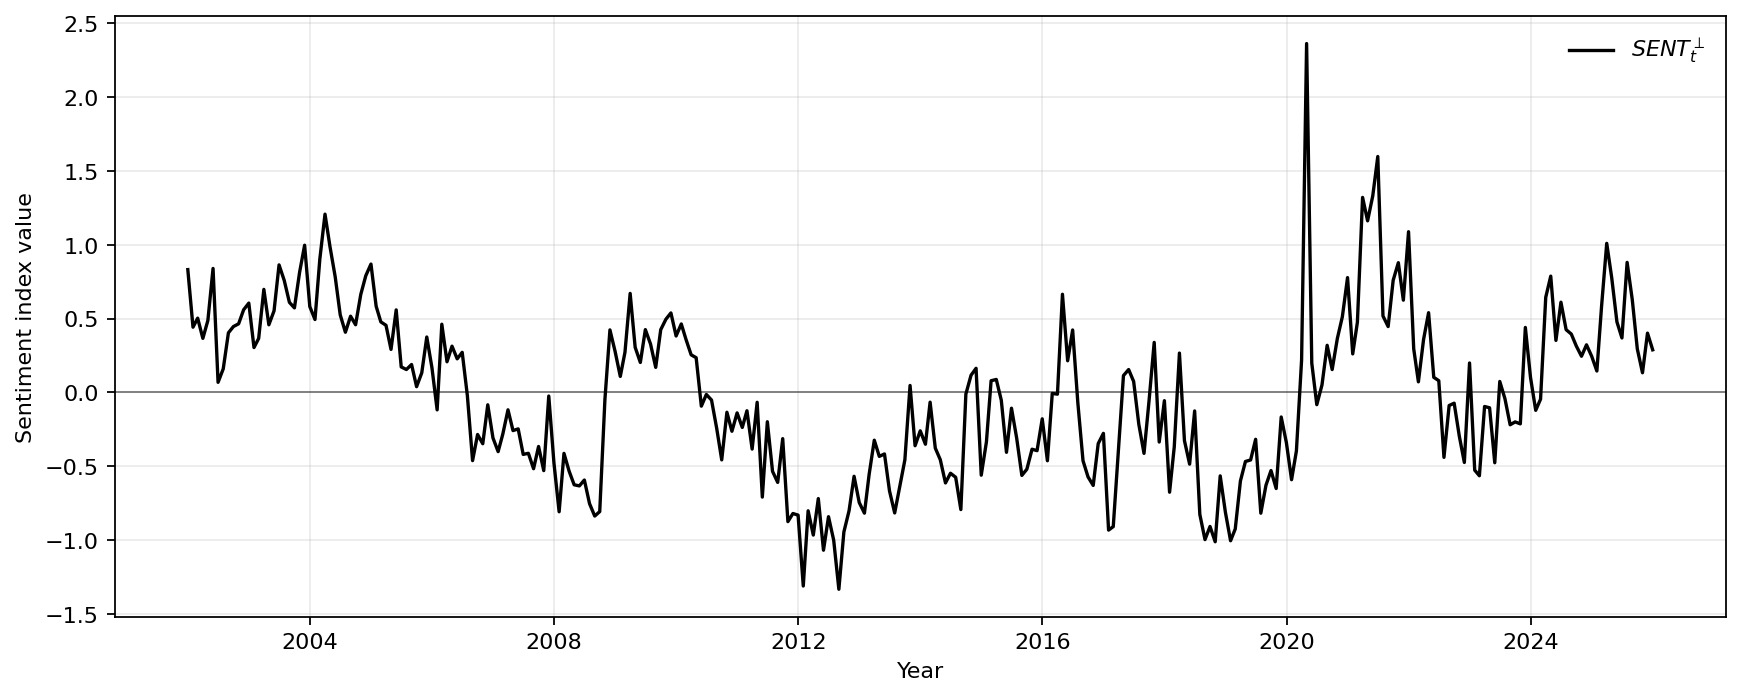
\includegraphics[width=\textwidth]{outputs/final_sentiment_sweden/final_sentiment_orth_div_premium_over_time.png}
    \caption{Macro-orthogonalised Swedish dividend-premium sentiment index}
    \label{fig:sentiment_orth_over_time}
    \figurenote{The figure plots \var{SENT^{\perp}_{t}}.}
\end{figure}

The largest observation occurs in the Covid crisis window, peaking in April 2020 after the March 2020 market shock. The spike is too large to read as ordinary optimism alone, and it likely reflects an extreme combination of survey movements, market activity, and macro-residualised proxy behavior during an unusual market episode. The spike is retained in \var{SENT^{\perp}} because the Covid period is an economically real stress episode rather than a coding error. The Covid-winsorised robustness check for the indices is reported in \Cref{fig:appendix_covid_winsorised_sentiment_indices,tab:appendix_covid_winsorised_sibley_characteristic_horizon} in the appendix. The adjustment does not materially change the composition or predictive ability of \var{SENT^{\perp}_{t}}.

\subsubsection{Sentiment against OMXS30}
\var{SENT^{\perp}_{t}} is placed against the large-cap Swedish market stress, as shown in \Cref{fig:omxs30_sentiment_drawdowns}. Elevated sentiment is followed by weak aggregate returns around the 2021--2022 market decline. Other drawdowns occur when \var{SENT^{\perp}_{t}} is moderate, and some high-sentiment observations are followed by no immediate large OMXS30 decline. The aggregate index relation is weaker than the cross-sectional prediction tested below.

\begin{figure}[H]
    \centering
    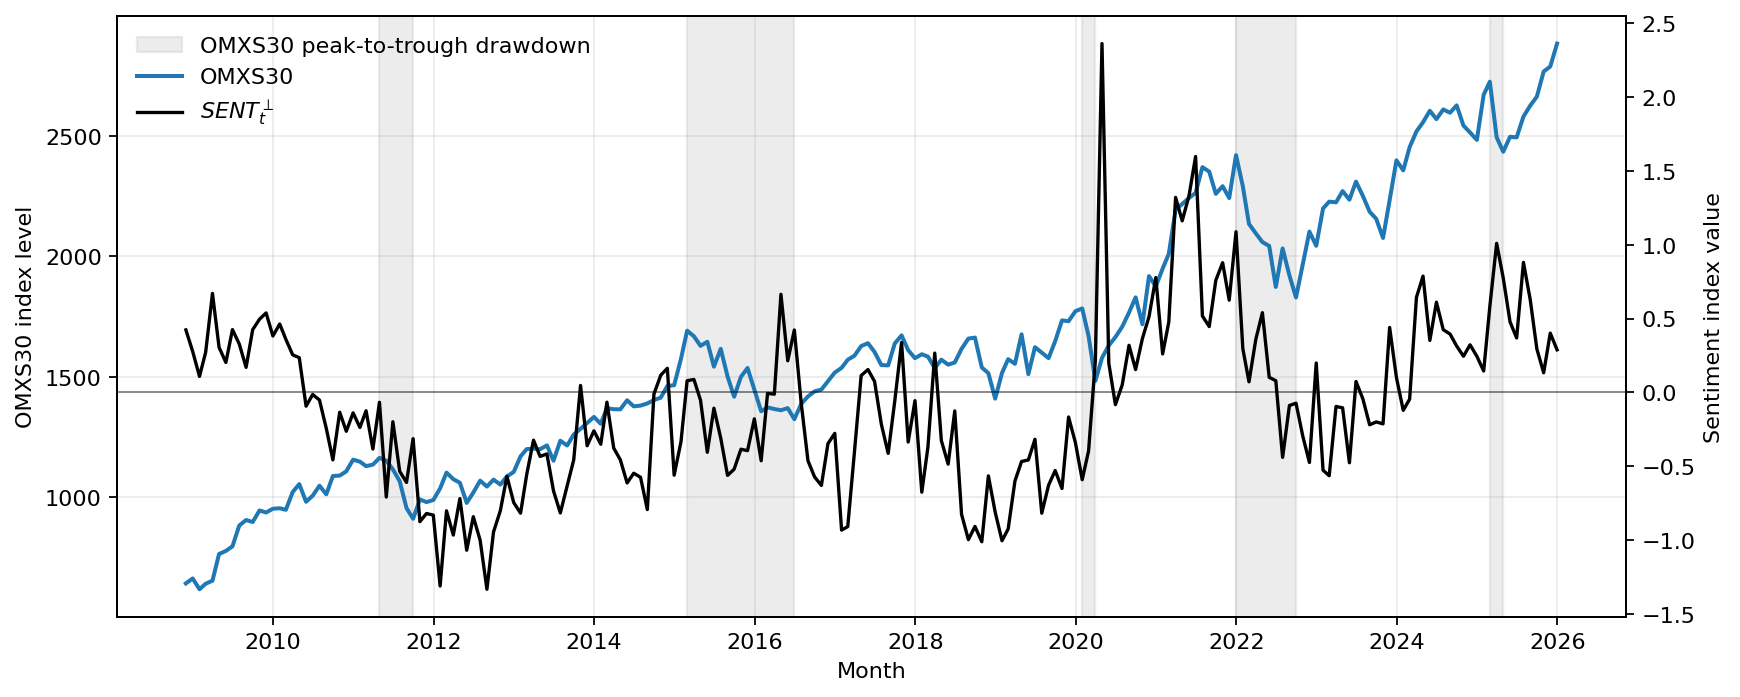
\includegraphics[width=\textwidth]{outputs/final_sentiment_sweden/final_omxs30_sent_orth_drawdowns_over_time.png}
    \caption{OMXS30 and macro-orthogonalised sentiment during major drawdowns}
    \label{fig:omxs30_sentiment_drawdowns}
    \figurenote{The blue line is the OMXS30 adjusted index level on the left axis. The black line is \var{SENT^{\perp}_{t}} on the right axis. Grey areas mark the five largest peak-to-trough OMXS30 drawdowns in the monthly OMXS30 series.}
\end{figure}

OMXS30 is a large-cap benchmark made up of liquid, established Swedish firms. The mechanism in \citet{baker2006sentiment} predicts larger sentiment effects in firms whose values are harder to estimate and harder to arbitrage, not necessarily in a blue-chip index dominated by larger firms with more durable cash-flow profiles. The sentiment index moves through important Swedish stress periods, without corresponding prior spikes in \var{SENT^{\perp}}. Selected standardised proxy panels around the same drawdowns are reported in \cref{fig:appendix_omxs30_proxy_drawdown_panels}.

\subsection{Constructed Portfolios}
The final directional portfolio design uses eleven characteristics: \var{ME}, age, risk, \var{IVOL^{FF3}}, non-dividend-payer status, unprofitable status, \var{E+BE}, \var{PPE/A}, \var{GS}, \var{ILLIQ}, and \var{XTURN}. 

\begin{table}[H]
    \centering
    \caption{Directional portfolio definitions}
    \label{tab:directional_portfolios}
    \scriptsize
    \begin{tabularx}{\textwidth}{lXl}
        \toprule
        Firm characteristic & Sentiment-prone leg & Directional spread \\
        \midrule
        \var{ME} & Small firms & Low minus high \\
        \var{risk} & High total volatility & High minus low \\
        \var{IVOL^{FF3}} & High three-factor idiosyncratic volatility & High minus low \\
        Age & Young firms & Low minus high \\
        Non-dividend payer & Non-payers & Non-payers minus payers \\
        Unprofitable & Non-positive earnings firms & Unprofitable minus profitable \\
        \var{E+BE} & Low profitability & Low minus high \\
        \var{PPE/A} & Low tangibility & Low minus high \\
        \var{GS} & High sales growth & High minus low \\
        Illiquidity & High Amihud illiquidity & High minus low \\
        Turnover & Low share turnover & Low minus high \\
        \bottomrule
    \end{tabularx}
    \tablenote{For continuous characteristics, low minus high means \var{P01-P10}; high minus low means \var{P10-P01}. Binary characteristics use their two natural groups.}
\end{table}

The directional spread is always the return on the sentiment-prone side minus the return on the sentiment-insensitive side. A negative coefficient on lagged sentiment means that the sentiment-prone portfolio earns lower subsequent returns after high sentiment. Negative coefficients are the hypothesis-consistent sign in the spread tests based on \citet{baker2006sentiment}. The later leg-decomposition tables estimate the two component legs separately.

As stated earlier, H1 requires lagged sentiment to predict future relative returns, while H2 requires the negative relation to be strongest in the portfolios with subjective valuations or limits to arbitrage. H3 requires the sentiment-prone leg to carry stronger negative predictability than the sentiment-insensitive leg.

Several spreads load on the same underlying part of the Swedish cross-section, as shown in \Cref{fig:spread_correlation_heatmap} in the appendix. The IVOL spread is strongly related to total risk, and size is also closely related to illiquidity and dividend status. The sales-growth spread is only weakly correlated with the main risk and size spreads. The results describe a connected cluster of small, risky, illiquid, non-dividend-paying firms plus a more separate growth-opportunity characteristic, rather than eleven independent tests.

\subsection{Empirical findings: Directional Spreads}
The Baker-Wurgler-style spread tests give selective support for sentiment-related return predictability in Sweden. Beginning-of-period \var{SENT^{\perp}} predicts lower future returns for several sentiment-prone legs relative to their sentiment-insensitive counterparts, but the findings are concentrated in specific firm characteristics. The strongest results are total risk, \var{IVOL^{FF3}}, size, low tangibility, and non-dividend-payer status. Unprofitable firms and young firms provide weaker horizon-dependent support. Low profitability, sales growth, illiquidity, and low turnover do not support the same interpretation.

\subsubsection{Factor-Adjusted empirical findings}
Each coefficient measures the percentage-point change in a future directional spread associated with a one-unit increase in lagged sentiment. Every spread is defined as the sentiment-prone leg minus the sentiment-insensitive leg, so a negative coefficient means that high sentiment predicts lower future returns for the sentiment-prone leg relative to the sentiment-insensitive leg. The \var{SENT^{\perp}} estimates across all horizons are reported in \cref{tab:sent_orth_predictive_overview}. Stars on coefficients mark HAC significance at the 10, 5, and 1\% levels.

\begin{table}[!htbp]
\centering
\caption{Overview of \var{SENT^{\perp}} predictive regression coefficients by horizon}
\label{tab:sent_orth_predictive_overview}
\scriptsize
\setlength{\tabcolsep}{3pt}
\begin{tabular*}{\textwidth}{@{\extracolsep{\fill}}lllllllll@{}}
\toprule
Characteristic & \multicolumn{2}{c}{1 month} & \multicolumn{2}{c}{3 months} & \multicolumn{2}{c}{6 months} & \multicolumn{2}{c}{12 months} \\
\cmidrule(lr){2-3}\cmidrule(lr){4-5}\cmidrule(lr){6-7}\cmidrule(lr){8-9}
 & Coef. & HAC $t$ & Coef. & HAC $t$ & Coef. & HAC $t$ & Coef. & HAC $t$ \\
\midrule
\multicolumn{9}{l}{\textit{Panel A. Size, Age, and Risk}} \\
\var{ME} & -1.34\textsuperscript{*} & -1.90 & -2.44 & -1.38 & -6.55\textsuperscript{**} & -2.39 & -14.04\textsuperscript{***} & -3.15 \\
\var{Age} & -0.38 & -0.80 & -1.06 & -0.79 & -2.86 & -1.23 & -8.37\textsuperscript{**} & -2.29 \\
$\sigma$ & -2.60\textsuperscript{***} & -3.50 & -6.49\textsuperscript{***} & -3.56 & -12.08\textsuperscript{***} & -4.30 & -19.65\textsuperscript{***} & -4.43 \\
\var{IVOL^{FF3}} & -2.24\textsuperscript{***} & -2.69 & -5.60\textsuperscript{***} & -2.97 & -11.74\textsuperscript{***} & -4.05 & -18.42\textsuperscript{***} & -3.75 \\
\midrule
\multicolumn{9}{l}{\textit{Panel B. Profitability and Dividend Policy}} \\
\var{E+BE} & -0.44 & -0.64 & 0.43 & 0.34 & 0.41 & 0.18 & 0.08 & 0.02 \\
\var{Unprofitable} & -0.54 & -0.96 & -1.11 & -1.36 & -2.50\textsuperscript{*} & -1.84 & -4.86\textsuperscript{***} & -3.04 \\
\var{Nonpayer} & -0.63\textsuperscript{**} & -2.24 & -1.88\textsuperscript{**} & -2.46 & -3.58\textsuperscript{***} & -2.88 & -4.96\textsuperscript{***} & -2.80 \\
\midrule
\multicolumn{9}{l}{\textit{Panel C. Tangibility and Growth Opportunities}} \\
\var{PPE/A} & -1.27\textsuperscript{***} & -2.99 & -4.46\textsuperscript{***} & -3.86 & -8.34\textsuperscript{***} & -4.21 & -15.27\textsuperscript{***} & -4.83 \\
\var{GS} & -0.80 & -1.33 & -0.88 & -0.64 & -1.41 & -0.55 & -3.21 & -0.61 \\
\midrule
\multicolumn{9}{l}{\textit{Panel D. Trading Frictions}} \\
\var{ILLIQ} & -0.30 & -0.67 & -0.03 & -0.03 & -1.32 & -0.65 & -2.58 & -0.72 \\
\var{XTURN} & -0.11 & -0.16 & 1.04 & 0.62 & 1.91 & 0.67 & 4.46 & 1.23 \\
\bottomrule
\end{tabular*}
\tablenote{Each coefficient is from the factor-adjusted predictive regression using lagged \var{SENT^{\perp}}. Coefficients are percentage-point effects on future sentiment-prone-minus-insensitive directional-spread returns. HAC t-statistics use Newey-West standard errors. Negative coefficients are theory-consistent for all listed spreads. Coefficient stars mark HAC significance at 10\%, 5\%, and 1\%.}
\end{table}

The coefficient for total risk ($\sigma$) is negative and significant in every horizon, growing from -2.60 at 1 month to -19.65 at 12 months. \var{IVOL^{FF3}} follows the same pattern, with significant negative coefficients from 1 to 12 months and a 12-month coefficient of -18.42. These two characteristics give the cleanest support for H2 because high total risk and high idiosyncratic volatility can be interpeted as proxies for valuation uncertainty and arbitrage risk.

The small-minus-large coefficient for size and age is negative in every horizon, but the the coefficients only become statistically significant at 6 and 12 months. The 12-month coefficient of -14.04 means that high \var{SENT^{\perp}} predicts lower future returns for small firms relative to large firms over the following year. Young firms also have negative coefficients in every horizon, but only the 12-month estimate is statistically supported. The age result therefore reinforces the long-horizon pattern, while size is the more statistically significant characteristic within this group.

Unprofitable firms have negative coefficients in all horizons and become statistically supported at 6 and 12 months, which is consistent with the Baker-Wurgler prediction that weak cash-flow anchors make valuation more sentiment sensitive. Low profitability measured by \var{E+BE} gives the opposite reading. Its coefficients turn positive from 3 to 12 months and are statistically weak. Non-dividend payers have negative and statistically significant coefficients in every horizon, reaching -4.96 at 12 months. This supports H2, although the result is interpreted cautiously because \var{DIVP} is one of the sentiment proxies used to construct \var{SENT^{\perp}}.

Tangibility is one of the most stable results in the section. Low-tangibility firms have significant negative coefficients at every horizon, with the 12-month coefficient reaching -15.27. This is consistent with the view that firms with fewer hard assets are harder to value and more exposed to sentiment-related repricing. Sales growth has the expected negative sign in every horizon, but the HAC t-statistics are weak throughout, making it statistically insignificant.

Trading frictions are the weakest part of the directional-spread regressions. Illiquidity has the expected negative sign in every horizon, but the coefficients are small and insignificant at the 10\% level. The coefficients of Turnover are more problematic, as they turn positive from 3 to 12 months. The 12-month coefficient is 4.46, which is inconsistent with the expected reversal pattern. The trading-friction empirical findings therefore do not support H2 in the same way as risk, \var{IVOL^{FF3}}, size, low tangibility, and dividend status.

\subsubsection{Raw Versus Macro-Adjusted Sentiment}
The empirical findings rely heavily on using \var{SENT^{\perp}} rather than raw \var{SENT}. At the 12-month horizon, the average coefficient is -7.89 for \var{SENT^{\perp}} and -4.00 for \var{SENT}. The share of characteristics with a theory-consistent 5\% result is 0.64 for \var{SENT^{\perp}} at 12 months, compared with 0.09 for \var{SENT}. The raw-versus-orthogonalised horizon summary is reported in \cref{tab:results_by_horizon} in the appendix, and the full horizon tables comparing \var{SENT} and \var{SENT^{\perp}} are reported in \cref{tab:bw2006_horizon_1m,tab:bw2006_horizon_3m,tab:bw2006_horizon_6m,tab:bw2006_horizon_12m} in the appendix.

Raw \var{SENT} gives strong statistical support for low tangibility and some short-horizon statistical significance for low turnover and sales growth, but it does not reproduce the strongest risk and IVOL pattern. At 12 months, the raw total-risk and \var{IVOL^{FF3}} coefficients are negative but statistically insignificant, with HAC t-statistics of -1.09 and -1.07. The same characteristics under \var{SENT^{\perp}} have HAC t-statistics of -4.43 and -3.75. The statistically significant empirical findings therefore comes mainly from the macro-adjusted sentiment state rather than from the raw common proxy component.

This differs from \citet{baker2006sentiment}, where raw and orthogonalised sentiment generally preserve the same message for the central speculative-firm spreads. In the Swedish results, \var{SENT} appears more closely tied to survey confidence and broad confidence-cycle variation, while \var{SENT^{\perp}} loads more strongly on residualised market-based proxies such as \var{DIVP}, turnover, and financing composition. The Swedish empirical findings resembles Baker-Wurgler most clearly for risk, \var{IVOL^{FF3}}, size, and dividend status, but the pattern is narrower and more dependent on macro adjustment. The compositional difference of the two indices can be seen in \Cref{tab:sentiment_pca_raw_orth_comparison}.

\subsubsection{Multiple Testing and Factor-Control Robustness}
The 44 \var{SENT^{\perp}} spread tests combine eleven characteristics and four horizons. The 44 spread tests are treated as one family, as shown in Benjamini-Hochberg false-discovery-rate correction to the one-sided expected-sign HAC p-values, \Cref{tab:fdr_primary_spread_tests}. This correction addresses the risk that isolated significant coefficients arise from testing many related characteristics and horizons.

\begin{table}[H]
    \centering
    \caption{Multiple-testing diagnostic for primary \var{SENT^{\perp}} spread tests}
    \label{tab:fdr_primary_spread_tests}
    \scriptsize
    \begin{tabularx}{\textwidth}{lrrr>{\raggedright\arraybackslash}X}
        \toprule
        Horizon & HAC 5\% count & FDR 10\% count & FDR 5\% count & Characteristics surviving FDR 5\% \\
        \midrule
        1 month & 5 & 5 & 4 & Total risk, low tangibility, \var{IVOL^{FF3}}, non-dividend payer \\
        3 months & 4 & 4 & 4 & Low tangibility, total risk, \var{IVOL^{FF3}}, non-dividend payer \\
        6 months & 6 & 6 & 5 & Total risk, low tangibility, \var{IVOL^{FF3}}, non-dividend payer, small firms \\
        12 months & 7 & 7 & 7 & Low tangibility, total risk, \var{IVOL^{FF3}}, small firms, unprofitable, non-dividend payer, young firms \\
        \bottomrule
    \end{tabularx}
    \tablenote{HAC 5\% count reports unadjusted one-sided expected-sign HAC significance. FDR columns apply the Benjamini-Hochberg false-discovery-rate procedure to one-sided expected-sign normal p-values computed from the HAC t-statistics across the full 44-test family. The Benjamini-Hochberg procedure is defined as the expected share of statistically significant findings that are false positives. It sorts the p-values from smallest to largest, compares each p-value with a rank-based threshold, and keeps the largest set of tests that pass the false-discovery-rate cutoff.}
\end{table}

The risk, \var{IVOL^{FF3}}, low-tangibility, and non-dividend-payer results survive the 5\% FDR threshold at the shorter horizons, while small firms, unprofitable firms, and young firms enter the surviving set only at longer horizons. Low profitability, illiquidity, sales growth, and turnover do not survive the correction. The correction therefore supports the clustered interpretation of H2, but not a broad statement that sentiment-related predictability appears across all tested characteristics.

Sentiment-only findings are separated from factor-adjusted findings and reported in \Cref{tab:factor_control_robustness}. The coefficient on lagged sentiment is a conditional cross-sectional predictability estimate after contemporaneous market, size, value, and momentum factor returns are absorbed over the same holding horizon.

\begin{table}[H]
    \centering
    \caption{\var{SENT^{\perp}}: Robustness to factor controls}
    \label{tab:factor_control_robustness}
    \small
    \begin{tabular}{lrrrrrr}
        \toprule
        Horizon & Sent.-only coef. & Factor-adj. coef. & Change & Sent.-only \var{R^2} & Factor-adj. \var{R^2} & Change \var{R^2} \\
        \midrule
        1 month & -0.27 & -0.97 & -0.69 & 0.003 & 0.290 & 0.287 \\
        3 months & 0.07 & -2.04 & -2.12 & 0.010 & 0.336 & 0.326 \\
        6 months & -1.35 & -4.37 & -3.01 & 0.017 & 0.385 & 0.369 \\
        12 months & -5.24 & -7.89 & -2.65 & 0.042 & 0.478 & 0.436 \\
        \bottomrule
    \end{tabular}
    \tablenote{Each row averages the eleven directional-spread regressions for \var{SENT^{\perp}}. Sentiment-only and factor-adjusted regressions use the same sample. The factor-adjusted specification adds \var{RMRF}, \var{SMB}, \var{HML}, and \var{UMD}.}
\end{table}

Lagged \var{SENT^{\perp}} explains little spread variation on its own, with average \var{R^2} below 0.05 at every horizon. The factor-adjusted \var{R^2} is much higher, reaching 0.478 at 12 months, which means that market, size, value, and momentum returns account for a large part of the time-series movement in the directional spreads. The sentiment coefficient nevertheless becomes more negative after factor adjustment at every horizon. \var{SENT^{\perp}} therefore retains incremental predictive content after standard return factors have been absorbed.

The Baker-Wurgler-style spread results gives a qualified answer to the research question. Beginning-of-period \var{SENT^{\perp}} predicts relative future returns in the Swedish cross-section, which supports H1. The support for H2 is concentrated in risk, \var{IVOL^{FF3}}, size, low tangibility, and dividend status. Profitability, illiquidity, turnover, and sales growth keep the conclusion from becoming a general statement that sentiment predicts all theoretically sentiment-prone Swedish spreads.

\subsection{Empirical findings: Leg Decomposition}
\citet{stambaugh2012short} use leg-level anomaly returns to distinguish broad spread predictability from an overpricing mechanism. Their central result is that high sentiment predicts especially weak subsequent returns on the short legs of anomaly strategies, where short-sale impediments make overpricing harder to eliminate. The leg decomposition separates each directional spread into a sentiment-prone leg and a sentiment-insensitive leg. The sentiment-prone leg is the closest analogue to the Stambaugh short leg because it is the side expected to be most exposed to high-sentiment overpricing.

The empirical findings of the legs are separated, as shown in \Cref{tab:stambaugh_prone_leg_overview,tab:stambaugh_insensitive_leg_overview}. A directional spread can become negative because the sentiment-prone leg underperforms, because the sentiment-insensitive leg outperforms, or because both happen at the same time. The prediction is strongest when the sentiment-prone leg has a negative coefficient and the sentiment-insensitive leg does not carry most of the spread. A positive or statistically dominant sentiment-insensitive leg can still create a predictive directional spread, but it weakens the interpretation that high sentiment mainly overprices the hard-to-arbitrage side.

Total risk and \var{IVOL^{FF3}} provide the empirical findings clearest and most consistent with \citet{stambaugh2012short}. Their sentiment-prone leg coefficients are negative and statistically supported at every horizon in \cref{tab:stambaugh_prone_leg_overview}. At 12 months, the sentiment-prone leg coefficients are -15.56 for total risk and -13.43 for \var{IVOL^{FF3}}. The sentiment-insensitive legs are also positive and statistically supported in \cref{tab:stambaugh_insensitive_leg_overview}, so the spreads are reinforced by both legs rather than generated only by weak returns on the sentiment-prone side. The Stambaugh interpretation remains strongest for these two characteristics because the negative sentiment-prone leg is large, persistent, and statistically supported.

The small-firm sentiment-prone leg turns statistically supported at 6 and 12 months, with coefficients of -6.61 and -15.28. The young-firm sentiment-prone leg follows the same longer-horizon pattern, with coefficients of -3.70 and -8.85. Their sentiment-insensitive legs are close to zero and statistically weak. The empirical findings therefore points more directly to weak future returns on the sentiment-prone side than to a spread mechanically produced by strong returns in the sentiment-insensitive leg.

\begin{table}[!htbp]
\centering
\caption{Overview of \var{SENT^{\perp}} sentiment-prone leg coefficients by horizon}
\label{tab:stambaugh_prone_leg_overview}
\scriptsize
\setlength{\tabcolsep}{3pt}
\begin{tabular*}{\textwidth}{@{\extracolsep{\fill}}lllllllll@{}}
\toprule
Characteristic & \multicolumn{2}{c}{1 month} & \multicolumn{2}{c}{3 months} & \multicolumn{2}{c}{6 months} & \multicolumn{2}{c}{12 months} \\
\cmidrule(lr){2-3}\cmidrule(lr){4-5}\cmidrule(lr){6-7}\cmidrule(lr){8-9}
 & Coef. & HAC $t$ & Coef. & HAC $t$ & Coef. & HAC $t$ & Coef. & HAC $t$ \\
\midrule
\multicolumn{9}{l}{\textit{Panel A. Size, Age, and Risk}} \\
\var{ME} & -1.16 & -1.61 & -2.34 & -1.30 & -6.61\textsuperscript{**} & -2.31 & -15.28\textsuperscript{***} & -3.07 \\
\var{Age} & -0.54 & -1.55 & -1.27 & -1.22 & -3.70\textsuperscript{**} & -2.08 & -8.85\textsuperscript{**} & -2.53 \\
$\sigma$ & -1.79\textsuperscript{***} & -3.18 & -4.72\textsuperscript{***} & -3.24 & -8.70\textsuperscript{***} & -3.84 & -15.56\textsuperscript{***} & -3.50 \\
\var{IVOL^{FF3}} & -1.54\textsuperscript{**} & -2.28 & -4.01\textsuperscript{**} & -2.40 & -8.52\textsuperscript{***} & -2.97 & -13.43\textsuperscript{**} & -2.24 \\
\midrule
\multicolumn{9}{l}{\textit{Panel B. Profitability and Dividend Policy}} \\
\var{E+BE} & 0.34 & 0.91 & 1.49 & 1.58 & 1.59 & 0.97 & 2.96 & 1.05 \\
\var{Unprofitable} & 0.37 & 0.49 & 1.80 & 0.97 & 3.45 & 0.85 & 11.32 & 1.08 \\
\var{Nonpayer} & -0.17 & -0.62 & -0.72 & -1.05 & -1.52 & -1.52 & -1.84 & -1.22 \\
\midrule
\multicolumn{9}{l}{\textit{Panel C. Tangibility and Growth Opportunities}} \\
\var{PPE/A} & -0.18 & -0.41 & -1.07 & -0.96 & -1.44 & -0.82 & -3.15 & -1.01 \\
\var{GS} & -0.41 & -1.00 & -1.01 & -1.04 & -2.73 & -1.56 & -4.97 & -1.57 \\
\midrule
\multicolumn{9}{l}{\textit{Panel D. Trading Frictions}} \\
\var{ILLIQ} & 0.05 & 0.11 & 0.56 & 0.58 & -0.38 & -0.21 & -1.25 & -0.32 \\
\var{XTURN} & -0.31 & -0.83 & -1.17 & -1.04 & -2.71 & -1.43 & -4.42 & -1.21 \\
\bottomrule
\end{tabular*}
\tablenote{Each coefficient is from the factor-adjusted leg regression using lagged \var{SENT^{\perp}}. Coefficients are percentage-point effects on future returns for the sentiment-prone leg of each directional spread. Negative coefficients are theory-consistent under the Stambaugh-style overpricing interpretation. HAC t-statistics use Newey-West standard errors. Coefficient stars mark HAC significance at 10\%, 5\%, and 1\%.}
\end{table}

The sentiment-insensitive leg regressions change the interpretation of several strong spread results found in the prior section. Total risk and \var{IVOL^{FF3}} have positive and statistically supported sentiment-insensitive leg coefficients as well as negative sentiment-prone leg coefficients. Their spread results therefore come from both sides of the characteristic comparison, although the sentiment-prone leg findings remain strong enough to support the Stambaugh mechanism. Low tangibility is different. The 12-month low-tangibility spread is one of the strongest Baker-Wurgler-style results, but the leg decomposition shows that the high-tangibility sentiment-insensitive leg carries most of the effect. The low-tangibility sentiment-prone leg coefficient is -3.15 with a HAC t-statistic of -1.01 making is statistically insignificant, while the high-tangibility sentiment-insensitive leg is 12.60 with a HAC t-statistic of 5.82. Non-dividend payer results has the same structure in weaker form. Its sentiment-prone leg coefficient is negative but weak, while the dividend-payer sentiment-insensitive leg is positive and statistically supported.

\begin{table}[!htbp]
\centering
\caption{Overview of \var{SENT^{\perp}} sentiment-insensitive leg coefficients by horizon}
\label{tab:stambaugh_insensitive_leg_overview}
\scriptsize
\setlength{\tabcolsep}{3pt}
\begin{tabular*}{\textwidth}{@{\extracolsep{\fill}}lllllllll@{}}
\toprule
Characteristic & \multicolumn{2}{c}{1 month} & \multicolumn{2}{c}{3 months} & \multicolumn{2}{c}{6 months} & \multicolumn{2}{c}{12 months} \\
\cmidrule(lr){2-3}\cmidrule(lr){4-5}\cmidrule(lr){6-7}\cmidrule(lr){8-9}
 & Coef. & HAC $t$ & Coef. & HAC $t$ & Coef. & HAC $t$ & Coef. & HAC $t$ \\
\midrule
\multicolumn{9}{l}{\textit{Panel A. Size, Age, and Risk}} \\
\var{ME} & 0.17 & 1.05 & 0.10 & 0.26 & 0.28 & 0.42 & 0.62 & 0.43 \\
\var{Age} & -0.16 & -0.51 & -0.08 & -0.09 & -0.21 & -0.14 & -0.20 & -0.07 \\
$\sigma$ & 0.81\textsuperscript{**} & 2.12 & 2.07\textsuperscript{**} & 2.14 & 4.58\textsuperscript{***} & 2.67 & 7.78\textsuperscript{***} & 3.21 \\
\var{IVOL^{FF3}} & 0.70\textsuperscript{*} & 1.76 & 1.88\textsuperscript{**} & 1.96 & 4.51\textsuperscript{***} & 2.68 & 9.07\textsuperscript{***} & 2.91 \\
\midrule
\multicolumn{9}{l}{\textit{Panel B. Profitability and Dividend Policy}} \\
\var{E+BE} & 0.78 & 1.40 & 1.03 & 1.10 & 1.33 & 0.95 & 2.97 & 1.42 \\
\var{Unprofitable} & 0.74 & 1.49 & 1.35\textsuperscript{*} & 1.94 & 1.79\textsuperscript{**} & 2.22 & 3.88\textsuperscript{***} & 3.33 \\
\var{Nonpayer} & 0.46\textsuperscript{**} & 2.23 & 1.15\textsuperscript{*} & 1.90 & 2.18\textsuperscript{**} & 2.23 & 3.64\textsuperscript{***} & 2.60 \\
\midrule
\multicolumn{9}{l}{\textit{Panel C. Tangibility and Growth Opportunities}} \\
\var{PPE/A} & 1.10\textsuperscript{***} & 3.24 & 3.42\textsuperscript{***} & 4.15 & 6.82\textsuperscript{***} & 4.73 & 12.60\textsuperscript{***} & 5.82 \\
\var{GS} & 0.39 & 0.91 & -0.24 & -0.22 & -1.30 & -0.82 & -1.83 & -0.64 \\
\midrule
\multicolumn{9}{l}{\textit{Panel D. Trading Frictions}} \\
\var{ILLIQ} & 0.35\textsuperscript{*} & 1.95 & 0.59 & 1.31 & 1.09 & 1.40 & 1.99\textsuperscript{*} & 1.94 \\
\var{XTURN} & -0.21 & -0.38 & -2.03 & -1.50 & -4.68\textsuperscript{**} & -2.28 & -9.64\textsuperscript{***} & -3.50 \\
\bottomrule
\end{tabular*}
\tablenote{Each coefficient is from the factor-adjusted leg regression using lagged \var{SENT^{\perp}}. Coefficients are percentage-point effects on future returns for the sentiment-insensitive leg of each directional spread. Positive coefficients indicate that high sentiment is followed by stronger returns for the more sentiment-insensitive side. HAC t-statistics use Newey-West standard errors. Coefficient stars mark HAC significance at 10\%, 5\%, and 1\%.}
\end{table}

Sales growth, illiquidity, and low turnover have negative 12-month sentiment-prone leg coefficients, but the findings are statistically insignificant. The sales-growth sentiment-prone leg coefficient is -4.97 with a HAC t-statistic of -1.57. Illiquidity is close to zero in statistical terms. Low turnover is harder to interpret because both legs are negative at 12 months, and the sentiment-insensitive leg is much more negative than the sentiment-prone leg. Low-profitability and unprofitable firms fail the sentiment-prone leg test. Their 12-month sentiment-prone leg coefficients are positive, which conflicts with the prediction that high sentiment should be followed by lower returns on the sentiment-prone side.

The empirical findings follows the pattern, that \citet{stambaugh2012short} finds, for risk, \var{IVOL^{FF3}}, and size. Those characteristics combine negative spread coefficients with negative sentiment-prone-leg coefficients, so they support both the Baker-Wurgler cross-sectional prediction and the stricter Stambaugh overpricing-asymmetry interpretation. Age gives a weaker version of the same pattern.

Low tangibility and dividend status support the Baker-Wurgler spread prediction more clearly than the Stambaugh leg prediction. Their spread coefficients indicate that sentiment predicts relative returns across Swedish characteristic portfolios, but their leg decomposition assigns a large part of the predictive relation to the sentiment-insensitive leg. The results still support H1 because they show cross-sectional predictability, but they provide weak and contradictory evidence for H3 because the strict short-leg asymmetry mechanism requires stronger negative predictability in the sentiment-prone leg.

\var{SENT^{\perp}} predicts Swedish cross-sectional return differences, which supports H1. Predictability is strongest in characteristics linked to risk, idiosyncratic volatility, and size, which supports H2 for firms where arbitrage risk and valuation uncertainty are most visible. H3 receives narrower support. Risk, \var{IVOL^{FF3}}, and size fit the predicted sentiment-prone-leg pattern most clearly. Low tangibility and dividend status remain important for H1 and H2, but their leg patterns show that the sentiment-insensitive leg contributes materially. Profitability and turnover are inconsistent with a broad H3 interpretation, while illiquidity and sales growth provide weak support. The empirical findings is therefore best interpreted as selective sentiment-related cross-sectional predictability, rather than a uniform overpricing-asymmetry pattern. There is therefore not broad support for H3.

\subsection{Robustness}
HAC/Newey-West standard errors and moving-block bootstrap t-statistics adjust the primary inference for heteroskedasticity, serial correlation, and time-series dependence in overlapping monthly return windows. Those corrections improve the coefficient-level inference, but they do not fully address the pattern that the expected-signed t-statistics rise with the return horizon. Coefficients can reasonably be expected to be larger over longer compounded horizons, but stronger t-statistics at longer horizons raise the possibility that persistent sentiment states and repeated holding-period observations make the make the empirical findings from \var{SENT^{\perp}} look stronger than a strictly non-overlapping design would imply. To address this concern, two robustness tests are conducted. They provide a check on whether the main results are overstated by overlapping returns or persistent sentiment episodes.

First, non-overlapping horizon regressions split the sample into \var{h} calendar-offset subsamples for each return horizon \var{h},
\begin{equation}
    \mathcal{T}_{h,o}=\{t: m(t)-o \equiv 0 \pmod h\}, \qquad o=0,\ldots,h-1,
\end{equation}
where \var{m(t)} is the monthly time index. The predictive regression is then re-estimated separately in each offset subsample. At the 12-month horizon, this produces twelve regressions for each characteristic, beginning respectively in January, February, and so on. The offset design prevents adjacent observations from mechanically sharing most of the same future holding-period returns. The reported robustness statistics summarize the median coefficient and median expected-signed t-statistic across offsets, together with the fraction of offsets that retain the theory-consistent negative sign.

The 12-month non-overlapping robustness test addresses the horizon where repeated holding-period observations are most severe. The main reversal pattern survives this stricter design. Total risk, three-factor idiosyncratic volatility, low tangibility, small firms, unprofitable firms, young firms, and non-dividend payers all retain negative median coefficients and positive expected-signed median t-statistics. The strongest empirical findings remain concentrated in risk, idiosyncratic volatility, and low tangibility. Sales growth is correctly signed in most offset samples but weak. Low profitability, illiquidity, and low turnover do not provide comparable support. The non-overlapping regressions reduce the concern that the long-horizon results are mechanically driven by repeated overlapping return windows. This provides further supoort for H1 and H2.

\begin{table}[H]
    \centering
    \caption{Persistence robustness: 12-month non-overlapping horizon regressions}
    \label{tab:nonoverlap_robustness}
    \small
    \begin{tabular}{lllllr}
        \toprule
        Characteristic & Baseline coef. & Baseline t & Non-overlap coef. & Non-overlap t & Sign share \\
        \midrule
        Total risk & -19.65\textsuperscript{***} & 4.43 & -23.41\textsuperscript{***} & 5.25 & 1.00 \\
        IVOL (FF3) & -18.42\textsuperscript{***} & 3.75 & -23.72\textsuperscript{***} & 5.59 & 1.00 \\
        Low tangibility & -15.27\textsuperscript{***} & 4.83 & -17.34\textsuperscript{***} & 4.31 & 1.00 \\
        Small firms & -14.04\textsuperscript{***} & 3.15 & -15.53\textsuperscript{***} & 3.33 & 1.00 \\
        Unprofitable & -4.86\textsuperscript{***} & 3.04 & -6.99\textsuperscript{***} & 3.15 & 1.00 \\
        Young firms & -8.37\textsuperscript{**} & 2.29 & -10.02\textsuperscript{**} & 2.52 & 1.00 \\
        Non-dividend payer & -4.96\textsuperscript{***} & 2.80 & -5.27\textsuperscript{**} & 2.31 & 1.00 \\
        Sales growth & -3.21 & 0.61 & -3.42 & 0.44 & 0.67 \\
        Low profitability & 0.08 & -0.02 & -2.06 & 0.95 & 0.58 \\
        Illiquidity & -2.58 & 0.72 & -3.64 & 0.80 & 0.92 \\
        Low turnover & 4.46 & -1.23 & 4.99 & -1.51 & 0.25 \\
        \bottomrule
    \end{tabular}
    \tablenote{The \var{SENT^{\perp}} columns use the overlapping 12-month predictive regressions. The non-overlap columns report the median coefficient and median expected-signed HAC t-statistic across the twelve calendar-offset samples. Sign share is the fraction of offset regressions with the theory-consistent negative coefficient. Coefficient stars mark HAC significance at 10\%, 5\%, and 1\%.}
\end{table}

Second, sentiment-innovation regressions model the orthogonalised sentiment index as a first-order autoregressive process,
\begin{equation}
    SENT^{\perp}_{t} = a + \rho SENT^{\perp}_{t-1} + u_t,
\end{equation}
and the residual \var{u_t} is interpreted as the unexpected component of sentiment after controlling for its own persistence. The predictive regression is then re-estimated with \var{u_{t-1}} in place of \var{SENT^{\perp}_{t-1}}. The specification asks whether new information in sentiment predicts subsequent cross-sectional return spreads, rather than allowing a long high-sentiment regime to enter the regression repeatedly through a highly persistent level measure.

The AR(1) coefficient of \var{SENT^{\perp}} is 0.794, with an \var{R^2} of 0.634, confirming that sentiment is highly persistent. When the lagged sentiment level is replaced by the lagged AR(1) innovation, the results weaken substantially. The average expected-signed t-statistic is 1.27 at the 12-month horizon, compared with 2.22 in the overlapping level regression. Therefore, the results are better interpreted as predictability from persistent high- and low-sentiment regimes than from unexpected month-to-month sentiment shocks, of which there is no statistical support.

The Swedish innovation results are weaker than the corresponding sentiment-change results in \citet{baker2007}. Baker and Wurgler use sentiment changes to capture contemporaneous price pressure, while sentiment levels capture later reversal. In the Swedish tests, changes in \var{SENT^{\perp}} do not show comparable statistical support across the directional spreads. This narrows the interpretation of the level-based predictive findings. The empirical findings support sentiment-related return predictability more clearly than they support a monthly contemporaneous price-pressure channel.

\subsubsection{Extreme-Decile Constituent Reuse}
Extreme-decile portfolio regressions may repeatedly measure the same firms rather than a broad cross-section of Swedish equities. Repeated-firm exposure is most relevant for characteristics that are persistent by construction. Large firms tend to remain large, old firms remain old, tangible firms do not rapidly change their asset structure, and highly liquid firms often remain in the liquid tail of the distribution. If the same securities are repeatedly selected into the extreme legs, the predictive regressions may appear broader than they are.

The firm composition behind the directional extreme-leg portfolios is analysed by deconstructing each complete baseline predictive-regression observation into the underlying security-month-leg rows used inside the relevant future return window. Then how often companies and securities appear is counted across all directional legs, horizons, and regression windows. The directional legs contain 1,516 unique companies. After applying the regression requirements, the expanded regression-window exposure contains 1,461 unique companies.

The regressions reuse persistent characteristic portfolios, not independent firm identities each month. Persistent characteristic portfolios necessarily reuse firms when extreme deciles are formed on slow-moving characteristics such as size, age, tangibility, and liquidity. However, the empirical findings does not support the concern that the results are driven by a small set of repeatedly sampled firms. The most frequently reused company (Swedbank AB) accounts for 0.37\% of expanded regression-window exposure, while the top 50 companies together account for 13.74\%. Continuous portfolio legs are also nearly balanced by construction, whereas binary characteristics are naturally less balanced but still draw on broad firm groups. The extreme-decile design remains a broad characteristic-portfolio design.

\section{Discussion}
\var{SENT^{\perp}} provides selective evidence of sentiment-related return predictability in the Swedish equity cross-section. The support for H1 is clearest at the 6- and 12-month horizons, where high beginning-of-period sentiment is followed by lower relative returns for several sentiment-prone directional spreads. The pattern is concentrated rather than uniform, with the strongest evidence in total risk, \var{IVOL^{FF3}}, size, low tangibility, and dividend status.

The results give partial support to H2. The strongest predictive relations appear where the theory in \citet{baker2006sentiment} and \citet{baker2007} points most directly, namely among firms with subjective valuations and stronger limits to arbitrage. Total risk, idiosyncratic volatility, and size are the cleanest examples because they are directly connected to uncertainty, limited arbitrage capacity, and lower investor coverage. Low tangibility and dividend status also fit the broad Baker-Wurgler spread logic, although their leg patterns are less clean. Profitability, illiquidity, turnover, and sales growth provide weak or conflicting evidence for H2. 

However the firm characteristics of size, total risk, idiosynchratic volatility and dividend status are highly correlated, which implies that these characteristics capture the same underlying variation, and therefore, does not provide evidence for separate arbitrage and valuation difficulty, but rather the same phenomena.

The empirical findings in support of H3 are significantly narrower than for H1 and H2. A negative directional spread means that the sentiment-prone leg underperforms the sentiment-insensitive leg after high sentiment, but H3 requires more than a negative spread. It requires stronger negative predictability in the sentiment-prone leg itself, consistent with the short-sale asymmetry mechanism in \citet{stambaugh2012short}. The leg decomposition fits this mechanism most clearly for total risk, \var{IVOL^{FF3}}, and size. Low tangibility and dividend status remain important spread results, but their sentiment-insensitive legs contribute materially. These characteristics support cross-sectional predictability more clearly than the stricter overpricing-leg interpretation, which in no way is broadly supported.

The market contains many smaller and growth-oriented firms, but household ownership and market structure differ from the U.S. setting behind \citet{baker2006sentiment} and \citet{stambaugh2012short}. The empirical findings therefore look less like a broad transfer of U.S. sentiment results and more like a Swedish pattern in which sentiment-related predictability appears most clearly among smaller, riskier, and harder-to-arbitrage firms. The weak evidence for profitability, illiquidity, turnover, and sales growth suggests that the Baker-Wurgler mechanism is not directly transferable, and does not map evenly onto every Swedish characteristic sort. This coincides with the findings of \citet{finter2012german}, who show that countries exhibit different patterns in the cross-section of returns.

\subsection{Macro-Financial Contamination and Expanded Orthogonalisation}
\citet{sibley2012sentimental} critique the interpretation of the sentiment index in \citet{baker2006sentiment} rather than only its forecasting performance. They accept the that the index predicts cross-sectional returns, but challenges whether the predictive component is necessarily behavioral sentiment. \citet{sibley2012sentimental} state that investor sentiment is \enquote{strongly correlated with contemporaneous business cycle variables} and that about 63\% of the total variation in the index can be explained by such variables. They further conclude that their results \enquote{cast doubt on the notion of \enquote{sentiment} as a pure behavioral predictive factor}. Their decomposition separates the fitted business-cycle component, \var{SENTHAT_t}, from the residual component, \var{SENTRES_t}. In their return-predictability tests, the business-cycle component carries most of the spread and short-leg predictability, while the residual component is much weaker. 

The critique also applies to the orthogonalised sentiment index in \citet{baker2006sentiment}. Thus, it applies to the index (\var{SENT^{\perp}}) created in this thesis. Baker and Wurgler residualize their sentiment proxies against a limited macroeconomic control set before extracting the common component. Yet \citet{baker2007} also acknowledge that sentiment measures may be \enquote{contaminated by economic fundamentals}. Orthogonalisation against a small set of macro controls improves the interpretation of a composite index, while the tested object changes from raw optimism to residual sentiment-related market-state variation. A sentiment index inspired by \citet{sibley2012sentimental} is created to discuss this further.

\var{SENT^{\perp}} residualizes the selected Swedish sentiment proxies against \var{CPI}, \var{PPI}, industrial production, and unemployment. The Sibley-expanded index, \var{SENT^{S}_{t}}, uses the same seven sentiment proxies as \var{SENT^{\perp}}, but residualizes them against a broader macro-financial control set before PCA. The expanded controls are unemployment, monthly CPI growth, consumption growth, industrial-production growth, the short rate, the term spread, the value-weighted Swedish market return, monthly market volatility, and the share of zero-return stock-days. These controls enter as \var{UNEMP}, \var{dCPI}, \var{dCONS}, \var{dIND}, \var{TBILL}, \var{TERM}, \var{VWRETD}, \var{MKTVOL}, and \var{PCTZERO}.

Available monthly Swedish data support a narrower control set than the full specification in \citet{sibley2012sentimental}. Disposable personal income growth, a recession dummy, the default spread, and aggregate dividend yield are omitted because sufficiently consistent monthly Swedish series are not available for those concepts. The expanded orthogonalisation therefore keeps the Sibley logic for the controls that can be measured defensibly, while the remaining are excluded because of data limitations.

\var{SENT^{\perp}} and \var{SENT^{S}} have a correlation of 0.466. The positive correlation shows that they capture a related market state. The moderate magnitude shows that the broader macro-financial controls remove a large part of the \var{SENT^{\perp}} common component. The comparison therefore is of which conclusions survive a stricter definition of residual sentiment-related variation.

The Sibley-expanded index preserves the expected negative average coefficient at every horizon, but the magnitude and statistical support are much weaker. At the 12-month horizon, the average coefficient falls from -7.89 for \var{SENT^{\perp}} to -1.88 for \var{SENT^{S}}. The average expected-signed HAC t-statistic falls from 2.22 to 0.73, and the expected-signed bootstrap t-statistic falls from 2.08 to 0.68. The share of characteristics with a theory-consistent 5\% HAC result is only 0.09 under \var{SENT^{S}} at every horizon. Characteristic-horizon details are reported in \cref{tab:appendix_sibley_characteristic_horizon} in the appendix.

\begin{table}[H]
    \centering
    \caption{Sibley-style expanded macro orthogonalisation by horizon}
    \label{tab:sibley_macro_comparison}
    \scriptsize
    \begin{tabular}{lrllrllr}
        \toprule
        Horizon & \var{SENT^{\perp}} b & \var{SENT^{\perp}} HAC & \var{SENT^{\perp}} boot & \var{SENT^{S}} b & \var{SENT^{S}} HAC & \var{SENT^{S}} boot & \var{SENT^{S}} 5\% \\
        \midrule
        1 month & -0.97 & 1.62 & 1.62 & -0.50 & 0.75 & 0.68 & 0.09 \\
        3 months & -2.04 & 1.46 & 1.45 & -0.49 & 0.24 & 0.24 & 0.09 \\
        6 months & -4.37\textsuperscript{*} & 1.93 & 1.91 & -1.46 & 0.79 & 0.75 & 0.09 \\
        12 months & -7.89\textsuperscript{**} & 2.22 & 2.08 & -1.88 & 0.73 & 0.68 & 0.09 \\
        \bottomrule
    \end{tabular}
    \tablenote{Each row averages the eleven directional-spread regressions by horizon. HAC and boot columns report expected-signed t-statistics. Positive values support the sentiment-reversal hypothesis. Stars on mean coefficients are based on the expected-signed HAC t-statistic and are descriptive for horizon-level averages.}
\end{table}

The characteristic-level results show what survives the stricter macro adjustment. Low tangibility remains the strongest result under \var{SENT^{S}}, with a mean expected-signed HAC t-statistic of 2.90. Sales growth and low turnover improve somewhat relative to \var{SENT^{\perp}} but remain weak. The main \var{SENT^{\perp}} evidence for total risk, \var{IVOL^{FF3}}, size, non-dividend payers, and unprofitable firms weakens sharply. The mean expected-signed HAC t-statistic falls from 3.37 to 0.43 for \var{IVOL^{FF3}}, from 2.20 to 0.95 for size, from 2.59 to 0.11 for non-dividend payers, and from 1.80 to 0.09 for unprofitable firms. Low tangibility is the most robust characteristic under expanded macro residualisation, while much of the broader \var{SENT^{\perp}} support depends on the baseline macro adjustment for statistical significance. This shows that a lot of the predictive ability, that earlier in the thesis was associated with \var{SENT^{\perp}}, can in fact reasonably be explained rationally by the business cycle and changes in risk premia \citep{sharpe1964capital}. 

The Covid-winsorisation check shown in \cref{fig:appendix_covid_winsorised_sentiment_indices,tab:appendix_covid_winsorised_sibley_characteristic_horizon} in the appendix measures sensitivity to high-leverage crisis observations in the PCA construction. Before PCA, the experiment caps only the March 2020 raw \var{ESI_t} and \var{CCI_t} observations that exceed the four-standard-deviation event-window rule. The baseline \var{SENT^{\perp}} series changes little, while the Sibley-expanded series changes materially. 

The adjustment changes the 12-month Sibley-expanded average coefficient from -1.88 to -6.98, the expected-signed HAC t-statistic from 0.73 to 1.78, and the 5\% HAC significance share from 0.09 to 0.36. At the 3- and 6-month horizons, the expected-signed HAC t-statistic rises from 0.24 to 1.21 and from 0.79 to 1.72, respectively. Winsorizing two extreme datapoints for each raw proxy thus changes the composition and predictive power of \var{SENT^{S}} materially, showing that the residuals of the heavily orthogonalised index is very sensitive to minor changes in the raw data outputs. The adjusted \var{SENT^{S}} shown in \Cref{tab:appendix_covid_winsorised_sibley_characteristic_horizon} provides broader statistically significant support for \var{SENT^{\perp}} to actually capture 'sentiment'. In part providing a caveat to the critique of \var{SENT^{\perp}} from \citep{sibley2012sentimental}.

\subsection{Fixed PCA Weights and External Validity}
\citet{ung2024enhanced} criticize fixed PCA sentiment indices because proxy loadings may change over time and full-sample PCA weights can embed information that would have been unavailable at the forecast date. Their enhanced sentiment index, STV, estimates principal-component loadings in rolling 36-month windows. The rolling design lets the relative contribution of each proxy vary over time and market regimes, and avoids using future proxy observations when constructing the sentiment value used for prediction. Their empirical comparison is therefore closer to a real-time forecasting exercise than the fixed-weight index design in \citet{baker2006sentiment}.

The same limitation applies to \var{SENT^{\perp}}. The return regressions use lagged sentiment and future Swedish portfolio returns, so the dependent return outcomes do not enter the index construction. However, the PCA weights are estimated using the full proxy sample, which assumes that each Swedish proxy has a stable relation to the latent sentiment state. The index is therefore an in-sample measure of a historical sentiment-related state, not a real-time allocation signal or an out-of-sample forecasting model. 

The central limitation is external validity. The empirical findings based on \var{SENT^{\perp}} can support the claim that Swedish sentiment-related states are followed by in-sample cross-sectional return reversals. It cannot by itself show that the same index construction would forecast returns out of sample or work as a real-time trading signal. A rolling or recursive Swedish PCA would be the natural extension, but it would introduce additional choices about window length, component sign anchoring, minimum observations, and proxy availability. In a relatively short monthly Swedish sample, those choices would trade lower look-ahead risk for higher measurement noise. 

An attempt at constructing a valid rolling window PCA, index is described shortly in \Cref{app:alternative_sentiment_index_designs} in the appendix. Not significant predicitive relation was discovered. That, nevertheless, does not detract from the critique made by \citet{ung2024enhanced} of fixed PCA constructions. But it does show that rolling PCA windows increase the measurement difficulty of the latent object 'sentiment'.

\subsection{Factor Controls and Market-Efficiency Interpretation}
The weak performance of raw \var{SENT} changes the interpretation of the Swedish results. In \citet{baker2006sentiment}, the raw and macro-orthogonalised indices generally point in the same empirical direction. In the Swedish results, raw \var{SENT} gives weaker expected-signed evidence at every horizon, while \var{SENT^{\perp}} produces stronger and more consistent negative coefficients for risk, idiosyncratic volatility, dividend status, and size. Raw \var{SENT} is most closely related to survey confidence, while \var{SENT^{\perp}} loads more strongly on residualised market-based proxies such as turnover, financing composition, and \var{DIVP}. The pattern fits the critique in \citet{sibley2012sentimental}. A sentiment index can predict returns while still containing macro-financial information. The empirical findings in this thesis is strongest when the common component is first stripped of observable macro variation, which makes the result closer to residual sentiment-related market-state predictability than to a broad optimism measure.

The factor-control results change the role assigned to sentiment. Average explanatory power is very low in the sentiment-only regressions and rises sharply after adding \var{RMRF}, \var{SMB}, \var{HML}, and \var{UMD}. Swedish characteristic spreads therefore move strongly with market, size, value, and momentum variation. \citet{baker2006sentiment} include the same family of controls because the sentiment coefficient should be evaluated after standard return factors have been absorbed. In the asset-pricing tradition of \citet{fama1993common} and \citet{carhart1997persistence}, these controls capture common return components that can otherwise be mistaken for predictability.

The empirical findings are difficult to reconcile with a simple unconditional efficient-market benchmark, but it does not establish a tradable anomaly or definitive market inefficiency after transaction costs, shorting constraints, liquidity, and capacity. Under the efficient-market benchmark in \citet{fama1970efficient} and \citet{fama1991efficient}, and the systematic-risk logic in \citet{sharpe1964capital}, predictable cross-sectional return differences should either reflect compensation for risk or disappear through arbitrage. Factor controls remain imperfect, and the Sibley-style tests show that macro-financial contamination remains relevant. The most defensible interpretation is conditional and behavioral in spirit. Swedish sentiment-related states are followed by reversals in selected parts of the cross-section where \citet{baker2006sentiment} and \citet{stambaugh2012short} predict stronger sentiment sensitivity.

\subsection{Implications for Identification}
The Sibley-expanded results move the interpretation from structural sentiment identification to predictive cross-sectional results. \var{SENT^{\perp}} predicts Swedish directional spreads in the expected direction, especially for high-risk firms, high-\var{IVOL^{FF3}} firms, low-tangibility firms, small firms, and non-dividend payers. The expanded macro adjustment reduces the average 12-month coefficient from -7.89 to -1.88 and lowers the average expected-signed HAC t-statistic from 2.22 to 0.73. A critical reading is that \var{SENT^{\perp}} captures a sentiment-related market state with predictive content, while the behavioral component inside that state is only partially isolated.

The main identification problem comes from the economic content of the proxies themselves. Survey confidence, turnover, IPO activity, financing composition, and the dividend premium are plausible sentiment proxies because they move with optimism, speculative participation, hot-issue conditions, issuer timing, and demand for safer dividend-paying firms. The same proxies also move with expected cash flows, discount rates, risk appetite, financing conditions, and market liquidity. \citet{sibley2012sentimental} show that this ambiguity is empirically meaningful in the setting of \citet{baker2006sentiment} because a business-cycle component explains much of the variation and predictive content of the sentiment index. The Swedish correlation of 0.466 between \var{SENT^{\perp}_{t}} and \var{SENT^{S}_{t}} points to the same issue. The expanded controls remove a large part of the \var{SENT^{\perp}} sentiment state, and the return predictability weakens with it.

The Sibley-expanded index functions as a stress test of interpretation. A final decomposition of fundamentals and beliefs would require richer identifying variation and additional monthly Swedish data. Some expanded controls may also absorb channels through which sentiment affects prices. Market returns, volatility, liquidity, and term-structure conditions can reflect fundamentals, but they can also be part of the pricing environment in which optimistic demand becomes more or less powerful. The weaker \var{SENT^{S}_{t}} results restrict the interpretation of the \var{SENT^{\perp}} empirical findings and make a purely behavioral reading too strong.

The strongest remaining claim is conditional and cross-sectional. \var{SENT^{\perp}} is most informative where the theory predicts larger sentiment-related return differences, namely among firms with subjective valuations or stronger limits to arbitrage. \citet{baker2006sentiment} predict larger return patterns where \enquote{valuations are highly subjective and difficult to arbitrage}, and the Swedish results are strongest for risk, \var{IVOL^{FF3}}, size, low tangibility, and dividend status. A purely mechanical macro proxy would be expected to map less systematically onto the characteristic families in \citet{baker2006sentiment}. The empirical findings supports sentiment-related predictability in the Swedish cross-section, while the Sibley critique leaves the behavioral purity of the index unresolved.

The leg decomposition narrows the overpricing interpretation significantly. \citet{stambaugh2012short} argue that high sentiment should mainly predict weak returns on the overpriced side because short-sale impediments make overpricing harder to correct. The leg results fit that logic most clearly for risk, \var{IVOL^{FF3}}, and size. Low tangibility is strong in the spread regressions, but the sentiment-insensitive leg contributes materially, which makes it weaker evidence for a Stambaugh-style short-leg channel. Profitability, illiquidity, turnover, and sales growth give weaker or conflicting signals. The empirical findings support the spread prediction in \citet{baker2006sentiment} more strongly than the stricter Stambaugh overpricing-asymmetry prediction.

The contribution is a Swedish cross-sectional test of sentiment-related return predictability with an explicit Sibley qualification. \var{SENT^{\perp}} predicts future return differences among theoretically sentiment-prone Swedish equities, especially in the risk, idiosyncratic-volatility, and size dimensions. The predictive sentiment state combines investor optimism with macro-financial conditions to an extent that remains only partially separated by the identification design. The empirical findings answers whether the Swedish cross-section contains sentiment-related return patterns, while a structural separation of behavioral beliefs from macro-financial state variation remains outside the identification power of the analysis.

\section{Conclusion}
Beginning-of-period investor sentiment has a conditional predictive relation with relative future returns in the Swedish equity cross-section, as framed in the research question, but the evidence is selective. It appears mainly at 6- and 12-month horizons and is concentrated in total risk, \var{IVOL^{FF3}}, size, low tangibility, and dividend status.

The hypothesis predicting that beginning-of-period investor sentiment predicts relative future returns in the Swedish equity cross-section (H1), is supported for \var{SENT^{\perp}} after controlling for Swedish market, size, value, and momentum factors.

The hypothesis predicting that the abovementiod predictive relation is stronger for stocks with subjective valuations or limits to arbitrage (H2) receives partial support because the strongest predictive relations appear where valuation uncertainty and limits to arbitrage are most visible. Low profitability, illiquidity, turnover, and sales growth limit the conclusion. Sentiment-related predictability does not apply across the full characteristic set.

The hypothesis predicting that the negative predictive relation after high beginning-of-period sentiment is stronger for the sentiment-prone portfolio leg than for the sentiment-insensitive leg (H3) is not supported in the same degree. While several directional spreads are consistent with sentiment-related predictability, the leg-decomposition tests show that this predictability does not systematically arise from lower subsequent returns in the sentiment-prone leg. The leg decomposition gives the most significant sentiment-prone-leg results for risk, \var{IVOL^{FF3}}, and size. Low tangibility and dividend status remain important spread results, but the sentiment-insensitive leg contributes materially. The overpricing-asymmetry pattern is therefore weak to inconsistent.

Empirical findings in support of all three hypotheses are conditional on the use of \var{SENT^{\perp}}, as both the raw \var{SENT} and stricter, in terms of macro-orthogonalisation, \var{SENT^{S}} does not produce the same statistical significance.

\var{SENT} performs substantially worse than \var{SENT^{\perp}}. The raw index is more closely tied to survey confidence, while \var{SENT^{\perp}} loads more heavily on residualised market-based sentiment proxies such as turnover, financing composition, and the dividend premium. The empriical findings are therefore closer to residual sentiment-related market-state predictability than to a broad optimism measure.

Identification remains the main limitation. \var{SENT^{S}} shows that part of the predictive content in \var{SENT^{\perp}} is sensitive to broader macro-financial residualisation, and the full-sample PCA construction makes the index a historical measurement device rather than a real-time forecasting model. 

My contribution is a Swedish test of cross-sectional sentiment-related return predictability using a constructed sentiment index, characteristic-sorted portfolios, factor-adjusted predictive regressions, leg decomposition, and robustness checks for macro contamination and horizon dependence. The empirical findings of the thesis supports conditional association between beginning-of-period sentiment and future Swedish cross-sectional returns, while causal identification and the structural separation of behavioral sentiment, macro-financial state variation, and arbitrage constraints remain unresolved.

\section{Thesis Results in Perspective}
The findings point beyond the Swedish sample in two directions: external validity and mechanism. The external-validity question is which parts of the cross-sectional sentiment framework could travel to other markets. The mechanism question is how local sentiment, external sentiment, investor trading, financing conditions, and arbitrage constraints jointly produce the observed return predictability.

\subsection{External Validity and Market Structure}
External validity should be evaluated at several levels. The most transferable implication is the cross-sectional prediction in \citet{baker2006sentiment} and \citet{baker2007}. Sentiment-related predictability should be more visible among firms with subjective valuations and stronger limits to arbitrage. The Swedish results for risk, \var{IVOL^{FF3}}, and size fits that broad theoretical pattern and is therefore the part of the result most likely to travel across markets.

The second level is more specific to small open European markets. Sweden combines a concentrated large-cap segment with a broad population of smaller listed and growth-market firms. Similar Nordic or European markets may therefore show the same split between muted aggregate sentiment transmission and stronger cross-sectional predictability in smaller, riskier, and less easily arbitraged firms. \citet{finter2012german} show that European sentiment research can require country-specific measurement, which supports this market-by-market approach.

The least transferable object is the exact Swedish sentiment index. Proxy weights, IPO-market conditions, macro controls, ownership structure, and survey behavior are locally dependent. A German, Danish, Finnish, or U.S. implementation could preserve the same theoretical design while producing a different composite sentiment state. The broader implication is therefore not that Sweden replicates the U.S. research and findings mechanically. The findings suggest that the hard-to-value and hard-to-arbitrage prediction is portable, while the specific index construction is market-specific.

\subsection{Local, Regional, and Global Sentiment}
The next research problem is to decompose the predictive sentiment state. \citet{baker2012global} show that sentiment can contain both global and local components, while \citet{sibley2012sentimental} show that business-cycle information can carry much of the apparent sentiment predictability. A Swedish extension should therefore separate domestic Swedish sentiment from Nordic regional sentiment, U.S. sentiment spillovers, global risk appetite, foreign-investor flows, and macro-financial conditions.

Several channels are empirically distinct. Global sentiment spillovers would appear if international risk appetite predicts Swedish directional spreads even after controlling for local sentiment. Nordic spillovers would appear if sentiment states in similar small open markets move together and predict the same Swedish firm characteristics. U.S. spillovers are especially relevant for speculative, technology, growth, or high-risk firms that may be priced with reference to global risk narratives. Ownership-channel spillovers would require foreign-investor flow or ownership data, while listing-market spillovers would connect IPO activity and small-cap financing conditions across countries.

A natural research design would combine Swedish sentiment proxies with external sentiment indices, foreign-flow measures, and event windows around domestic and international macro announcements. Such a design could distinguish domestic optimism, imported sentiment, and macro-financial news absorption as sources of Swedish return predictability. The findings provide the Swedish cross-sectional pattern that such a decomposition would try to explain.

\subsection{From Predictability to Mechanism}
The strongest next step is a mechanism design. \var{SENT^{\perp}} predicts selected Swedish directional spreads, but direct data on trading constraints, investor clienteles, and belief disagreement would be needed to explain why those patterns arise. The short-sale asymmetry mechanism in \citet{stambaugh2012short} and the arbitrage-risk interpretation in \citet{stambaugh2015ivol} point to short interest, securities-lending supply, borrowing fees, and failed loan availability as the most direct data sources for the arbitrage-constraint channel.

Investor-clientele data would require trading or ownership changes by households, institutions, and foreign investors. Retail flow data would test whether high-sentiment states coincide with buying pressure in small, volatile, young, or otherwise sentiment-prone firms. Institutional and foreign ownership changes would show whether professional or international investors absorb or amplify sentiment-related pressure. Analyst disagreement, forecast dispersion, search intensity, news attention, mutual-fund flows, transaction costs, and liquidity measures would add datapoints on belief dispersion, attention, and implementability.

Financing-market data would sharpen the IPO and issuance channels. IPO allocation records, first-day trading data, post-listing ownership changes, and small-cap financing conditions would show whether hot-issue activity is connected to investor demand, issuer timing, or broader funding conditions. Event-based designs around sentiment shocks, macro announcements, or issuance waves would help distinguish persistent sentiment states from discrete information events.

\subsection{Future Research}
Three extensions follow most directly from the results. The first is a local-versus-global sentiment decomposition. Future research would need to estimate Swedish, Nordic, European, U.S., and global sentiment components jointly and test which component predicts the strongest Swedish characteristics.

The second extension is an investor-type channel. Future work could link sentiment states to household, institutional, and foreign trading flows, then test whether the sentiment-prone firms are bought or sold by the investor groups predicted by behavioral finance. That research would connect the Swedish results more directly to the retail-sentiment and attention mechanisms in \citet{kumar2006retail} and \citet{barber2008glitters}.

The third extension is a direct arbitrage-constraint test in Swedish small caps. Borrowing fees, lending supply, short interest, transaction costs, and liquidity would show whether the firms with stronger sentiment-related reversals are also the firms where mispricing is hardest to correct. That design would move the empirical findings from characteristic-based inference toward a direct test of the Stambaugh-style channel.

This thesis does not close the question of sentiment-driven mispricing in Sweden. It establishes that sentiment-related market-state variation has structured predictive content in selected parts of the Swedish cross-section. The next step is to identify the investor, trading, and financing channels through which that predictability arises.

\clearpage
\addcontentsline{toc}{section}{References}
\bibliographystyle{apalike}
\bibliography{behavioral_finance_exam}

\clearpage
\appendix
\section{Appendix}

\subsection{Appendix: Data}

\subsubsection{Daily and Monthly Market Source Resolution}
\label{app:market_source_resolution}

The monthly security panel is built from both daily and monthly market records. Before 2007, month-end observations are derived from the last valid daily trading record in each month. From January 2007 onward, the monthly dataset is the preferred price source when there is a valid price. Monthly returns are computed from adjusted month-end prices using the total-return factor, and market equity is measured as month-end price multiplied by shares outstanding. The monthly market panel is used for firm characteristics, factor controls, portfolio sorts, and predictive regressions.

\begin{figure}[H]
    \centering
    \includegraphics[width=\textwidth]{../outputs/eda_sweden_equity_market/monthly_market_composition_over_time.png}
    \caption{Monthly market-panel composition over time}
    \label{fig:appendix_monthly_market_composition}
    \figurenote{The figure reports the monthly composition of the filtered Swedish market panel used before empirical test-specific overlap requirements are applied.}
\end{figure}


\subsubsection{Accounting Filing Dates and Point-in-Time Fallback Lags}
\label{app:accounting_filing_lags}

Quarterly accounting observations are first converted into filing-level records and then into monthly point-in-time snapshots. A report is treated as available on the final filing date where available, otherwise on the preliminary filing date, and otherwise after a fallback lag from fiscal period end. Quarterly observations use a 90-day fallback lag and semiannual observations use a 180-day fallback lag. For each month-end, the latest available filing whose effective month-end is observable by that date is assigned. This timing prevents future accounting information from entering portfolio assignments, preventing data leakage.


\subsubsection{Raw Compustat Input-Field Coverage}

The raw Compustat extracts impose limits on which accounting characteristics from \citet{baker2006sentiment} can be measured in Sweden. Raw field coverage before any monthly carry-forward is applied is reported in \Cref{tab:fundamental_accounting_coverage}. Price, return-factor, and shares-outstanding fields are strongly covered in the market files, while daily trading volume is less complete. Balance-sheet fields needed for total assets, book-equity repair, and liabilities are broadly available, while revenue and tangible fixed-asset fields are usable but incomplete. \repo{revtq} is used as the single revenue input for the sales-growth characteristic, \var{GS}. Earnings coverage is strong when income before extraordinary items is used, but the alternative net-income fields are essentially unavailable in the extract. Dividend information is present only for a minority of raw firm-quarter records. External-finance fields are substantially weaker, with sale of common and preferred stock present in fewer than one third of firm-quarters, while repurchases and long-term debt issuance have very low coverage. Research and development expense and deferred-tax adjustment fields are absent from the saved Compustat extract.


\begin{table}[H]
\centering
\caption{Raw Compustat input-field coverage}
\label{tab:fundamental_accounting_coverage}
\scriptsize
\begin{tabularx}{\textwidth}{>{\raggedright\arraybackslash}X c c c}
\toprule
Title & Compustat Code & Raw-row availability & Coverage (\%) \\
\midrule
\multicolumn{4}{l}{\textit{Monthly market fields}} \\
Price Close - Monthly & prccm & 256,671 & 96.99\% \\
Trading Volume - Monthly & cshtrm & 211,442 & 79.90\% \\
\midrule
\multicolumn{4}{l}{\textit{Daily market, return, and liquidity fields}} \\
Price Close - Daily & prccd & 6,307,856 & 99.99\% \\
Shares Outstanding - Company & cshoc & 6,189,018 & 98.10\% \\
Trading Volume - Daily & cshtrd & 4,279,555 & 67.84\% \\
Total Return Factor & trfd & 6,308,333 & 99.99\% \\
\midrule
\multicolumn{4}{l}{\textit{Scale and revenue fields}} \\
Assets - Total & atq & 61,856 & 94.29\% \\
Sales/Turnover (Net) & saleq & 49,286 & 75.13\% \\
Sales/Turnover (Net), YTD & saley & 53,105 & 80.95\% \\
Revenue - Total & revtq & 58,650 & 89.40\% \\
\midrule
\multicolumn{4}{l}{\textit{Tangibility and investment fields}} \\
Property Plant and Equipment - Total (Net) & ppentq & 52,759 & 80.42\% \\
Capital Expenditures & capxy & 36,080 & 55.00\% \\
\midrule
\multicolumn{4}{l}{\textit{Earnings fields}} \\
Income Before Extraordinary Items & ibq & 61,071 & 93.09\% \\
Net Item - Total & nitq & 66 & 0.1\% \\
Income Before Extraordinary Items, YTD & iby & 65,418 & 99.72\% \\
Net Item - Total, YTD & nity & 452 & 0.69\% \\
\midrule
\multicolumn{4}{l}{\textit{Book-equity and balance-sheet fields}} \\
Common/Ordinary Equity - Total & ceqq & 51,639 & 78.72\% \\
Stockholders Equity $>$ Parent $>$ Index Fundamental $>$ Quarterly & seqq & 63,087 & 96.17\% \\
Stockholders Equity - Total & teqq & 49,564 & 75.55\% \\
Liabilities - Total & ltq & 61,836 & 94.26\% \\
Preferred/Preference Stock (Capital) - Total & pstkq & 498 & 0.76\% \\
Retained Earnings & req & 34,678 & 52.86\% \\
\midrule
\multicolumn{4}{l}{\textit{Dividend fields}} \\
Cash Dividends & dvy & 12,475 & 19.02\% \\
Dividends - Total & dvty & 6,213 & 9.47\% \\
Dividends - Total, quarterly & dvtq & 4,861 & 7.41\% \\
\midrule
\multicolumn{4}{l}{\textit{External-finance fields}} \\
Sale of Common and Preferred Stock & sstky & 18,083 & 27.56\% \\
Purchase of Common and Preferred Stock & prstkcy & 926 & 1.41\% \\
Long-Term Debt - Issuance & dltisy & 5 & 0.01\% \\
\midrule
\multicolumn{4}{l}{\textit{Fields not present in the extract}} \\
Research and Development Expense & not present & 0 & 0\% \\
Deferred Taxes and Investment Tax Credit & not present & 0 & 0\% \\
\bottomrule
\end{tabularx}
\tablenote{Coverage is measured before point-in-time monthly carry-forward and before portfolio formation. Accounting-field coverage uses the raw quarterly fundamentals denominator of 65,602 firm-quarter records identified by unique \repo{gvkey}/\repo{datadate} pairs. Monthly market-field coverage uses 264,645 raw security-month rows from the monthly price extract. Daily market-field coverage uses 6,308,719 raw security-day rows from the daily price extract. Fields marked as not present were not included in the saved WRDS extract used for the analysis.}
\end{table}


\subsubsection{Swedish Market Background Tables}


\begin{table}[H]
\centering
\caption{Largest OMXS30 Drawdowns in the Monthly OMXS30 Series}
\label{tabomxs30drawdowns}
\small
\begin{tabular}{lllrrr}
\toprule
Peak month & Trough month & Recovery month & Peak level & Trough level & Drawdown (\%) \\
\midrule
Dec. 2021 & Sep. 2022 & Feb. 2024 & 2,419.73 & 1,828.98 & -24.4 \\
Feb. 2015 & Jun. 2016 & Oct. 2019 & 1,691.03 & 1,323.58 & -21.7 \\
Apr. 2011 & Sep. 2011 & Jan. 2013 & 1,162.84 & 910.17 & -21.7 \\
Jan. 2020 & Mar. 2020 & Sep. 2020 & 1,783.26 & 1,482.43 & -16.9 \\
Feb. 2025 & Apr. 2025 & Oct. 2025 & 2,724.70 & 2,434.06 & -10.7 \\
\bottomrule
\end{tabular}
\tablenote{Drawdowns are computed from monthly adjusted close values. Recovery month is the first later month in which the index reaches or exceeds the previous monthly peak. The monthly OMXS30 series covers January 2009 to December 2025.}
\end{table}


\begin{table}[H]
\centering
\caption{Largest Companies in the Filtered Sweden Sample, December 2025}
\label{tabtopcompanies2025}
\small
\begin{tabularx}{0.92\textwidth}{Xlrr}
\toprule
Company & Sector & Market cap, SEK bn & Sample share (\%) \\
\midrule
Investor AB & Financials & 1,011.8 & 8.74 \\
Atlas Copco AB & Industrials & 790.1 & 6.82 \\
Volvo AB & Industrials & 601.9 & 5.20 \\
EQT AB & Financials & 449.2 & 3.88 \\
SEB AB & Financials & 393.8 & 3.40 \\
ASSA ABLOY AB & Industrials & 378.7 & 3.27 \\
Sandvik AB & Industrials & 377.1 & 3.26 \\
Swedbank AB & Financials & 363.5 & 3.14 \\
Saab AB & Industrials & 287& 2.48 \\
Hexagon AB & Information Technology & 284.2 & 2.45 \\
\bottomrule
\end{tabularx}
\tablenote{Market capitalisation is aggregated across listed share classes within company name. Sample share is measured relative to the filtered December 2025 Sweden sample.}
\end{table}


\subsection{Appendix: Methodology}

\begin{figure}[H]
    \centering
    \begin{tikzpicture}[
        font=\scriptsize,
        node distance=0.18cm,
        process/.style={
            draw=black!75,
            fill=black!4,
            rounded corners=1.5pt,
            line width=0.35pt,
            text width=0.91\textwidth,
            align=left,
            inner xsep=5pt,
            inner ysep=3pt
        },
        subbox/.style={
            draw=black!55,
            fill=white,
            rounded corners=1pt,
            line width=0.3pt,
            text width=0.405\textwidth,
            align=left,
            inner xsep=4pt,
            inner ysep=3pt
        },
        arrow/.style={
            -{Latex[length=2mm,width=1.2mm]},
            line width=0.35pt,
            draw=black!65
        }
    ]

    \node[process] (raw) {
        \textbf{1. Start with the raw inputs}\\[-1pt]
        Market data give prices, returns, shares and volume. Compustat gives quarterly accounting data and filing dates. Sentiment inputs cover \var{ESI}, \var{CCI}, turnover, IPO activity, financing composition and the dividend premium. Macro and rate data cover \var{CPI}, \var{PPI}, industrial production, employment, the 3-month rate and the 10-year yield.
    };

    \node[process, below=of raw] (filters) {
        \textbf{2. Keep the usable Sweden sample}\\[-1pt]
        Keep Swedish listed common equities with usable security-level return observations, positive prices, positive market equity, and the required market, accounting, sentiment and macro data.
    };

    \node[process, below=of filters] (ids) {
        \textbf{3. Keep company and security identifiers separate}\\[-1pt]
        \repo{company\_id} = country code + \repo{gvkey}. \repo{security\_id} = country code + \repo{gvkey} + \repo{iid}. Accounting measures are company-level, while prices, returns and portfolio assignments are security-level.
    };

    \node[process, below=of ids] (monthly) {
        \textbf{4. Build the monthly analysis panel}\\[-1pt]
        Resolve month-end prices. Before 2007, use the last valid daily observation in each month. From 2007 onward, use the monthly source. Then construct adjusted returns, market equity, the risk-free rate, Swedish factors and point-in-time accounting snapshots.
    };

    \node[process, below=of monthly, inner ysep=4pt] (charwrap) {
        \textbf{5. Build characteristics and sentiment}\\[-1pt]
        \begin{tikzpicture}[baseline=(firm.base)]
            \node[subbox] (firm) {
                \textbf{Firm characteristics}\\[-1pt]
                \var{ME}, age, total risk, \var{BE/ME}, profitability, dividend-payer status, \var{PPE/A}, sales growth, illiquidity, turnover, \var{IVOL}.
            };
            \node[subbox, right=0.035\textwidth of firm] (sent) {
                \textbf{Sentiment proxies}\\[-1pt]
                \var{ESI}, \var{CCI}, \var{TURN}, \var{NIPO}, \var{RIPO}, \var{ED\_RATIO}, \var{DIVP}. Residualize the selected proxies against macro controls and use PCA to form \var{SENT} and \var{SENT^{\perp}}.
            };
        \end{tikzpicture}
    };

    \node[process, below=of charwrap] (ports) {
        \textbf{6. Sort portfolios with lagged characteristics}\\[-1pt]
        Use one-month lagged characteristics. Continuous characteristics are sorted into Swedish monthly deciles; binary characteristics form two groups. Directional spreads are coded as sentiment-prone minus sentiment-insensitive, for example small--large, high \var{IVOL}--low \var{IVOL}, and low tangibility--high tangibility.
    };

    \node[process, below=of ports] (regs) {
        \textbf{7. Run the predictive tests}\\[-1pt]
        Regress future spread returns on lagged \var{SENT^{\perp}}. Decompose the same tests into sentiment-prone and sentiment-insensitive legs. Add \var{RMRF}, \var{SMB}, \var{HML} and \var{UMD} over matching 1-, 3-, 6- and 12-month horizons. Use Newey-West/HAC inference and bootstrap robustness.
    };

    \node[process, below=of regs] (interp) {
        \textbf{8. Interpret the results}\\[-1pt]
        Test whether high-sentiment states predict lower future returns for sentiment-prone Swedish stocks, and use the spread, leg and robustness empirical findings to assess H1, H2 and H3.
    };

    \draw[arrow] (raw) -- (filters);
    \draw[arrow] (filters) -- (ids);
    \draw[arrow] (ids) -- (monthly);
    \draw[arrow] (monthly) -- (charwrap);
    \draw[arrow] (charwrap) -- (ports);
    \draw[arrow] (ports) -- (regs);
    \draw[arrow] (regs) -- (interp);
    \end{tikzpicture}
    \caption{Empirical construction and testing pipeline.}
    \label{fig:appendix_empirical_pipeline_flowchart}
    \figurenote{The figure summarizes how raw Swedish market, accounting, sentiment, IPO, macroeconomic and interest-rate data are converted into the monthly security-level panel used for characteristic-sorted portfolio tests and predictive regressions.}
\end{figure}


\subsubsection{Factor-Construction Details}
\label{app:factor_construction_details}

Monthly factor returns are measured in percentage points and are constructed from the same Swedish security-month panel used in the characteristic sorts. Securities must pass the common-equity screen, have valid monthly returns, and have positive lagged market equity when value-weighted returns are computed. The factor audit table records breakpoints, constituent counts, lagged weight sums, equal-weighted leg returns, value-weighted leg returns, and thin-leg flags.

The Swedish 3-month interbank rate is converted from an annual percentage rate into the monthly risk-free proxy \var{RF^{3M}_t}. The value-weighted local market return, \var{R^{M,VW}_t}, is computed from Swedish common-equity returns using lagged market equity as the portfolio weight. The market excess return is
\begin{equation}
    RMRF_t = R^{M,VW}_t - RF^{3M}_t.
\end{equation}
The 10-year Swedish yield, \var{Y^{10Y}_t}, is retained as a macro-financial series, while \var{RF^{3M}_t} is the regression risk-free leg.

\var{SMB_t} is constructed from monthly Swedish size sorts. Wquities are sorted into low, middle, and high size buckets using the 30th and 70th percentile breakpoints of lagged market equity. The factor return uses the two extreme legs,
\begin{equation}
    SMB_t = R^{Small,VW}_t - R^{Big,VW}_t.
\end{equation}
The middle bucket is not used.

\var{HML_t} is constructed from monthly Swedish book-to-market sorts. Book equity comes from point-in-time accounting snapshots, while market equity comes from the resolved monthly market panel. The book-to-market signal is lagged before sorting. Equities are assigned to low, middle, and high book-to-market buckets using 30th and 70th percentile breakpoints. The factor return is
\begin{equation}
    HML_t = R^{High\ BE/ME,VW}_t - R^{Low\ BE/ME,VW}_t.
\end{equation}

\var{UMD_t} is constructed from monthly Swedish momentum sorts. The momentum signal compounds prior monthly returns while skipping the most recent month, following the convention that recent one-month reversals should be separated from medium-term momentum. Equities are sorted into loser, middle, and winner buckets using 30th and 70th percentile breakpoints of the lagged momentum signal. The factor return is
\begin{equation}
    UMD_t = R^{Winner,VW}_t - R^{Loser,VW}_t.
\end{equation}
For horizons of 1, 3, 6, and 12 months, forward factor windows match the compounded portfolio-return window from month \var{t} through month \var{t+h-1}.

Two auxiliary OLS regressions enter before the final predictive tests. The macro-orthogonalised sentiment index residualizes each selected sentiment proxy against Swedish macroeconomic controls,
\begin{equation}
    Z_{k,t}
    =
    a_k
    + b_{1k} CPI_t
    + b_{2k} PPI_t
    + b_{3k} IP_t
    + b_{4k} EM_t
    + e_{k,t}.
\end{equation}
The residuals \var{e_{k,t}} are standardised and passed into the PCA index construction. The residualisation step reduces business-cycle contamination in the sentiment proxies before the return-predictability tests are estimated.

\subsubsection{Robustness and Inference Implementation Details}
\label{app:robustness_implementation_details}

The non-overlapping robustness test re-estimates the directional-spread regression on calendar-offset subsamples. For horizon \var{h}, the sample is split into \var{h} subsamples according to the month index,
\begin{equation}
    m(t) \bmod h = k,
    \qquad
    k = 0,1,\ldots,h-1.
\end{equation}
Each offset subsample contains return windows that are separated by the full return horizon. The model is otherwise the same factor-adjusted predictive OLS regression as the primary specification. Reported statistics include median coefficients, median t-statistics, sign-consistency shares, and significance shares across offsets.

The sentiment-innovation test removes first-order persistence from \var{SENT^{\perp}} before prediction. The index is modelled as
\begin{equation}
    SENT^{\perp}_{t}
    =
    a
    +
    \rho SENT^{\perp}_{t-1}
    +
    u_t.
\end{equation}
The residual \var{u_t} is the innovation in sentiment, measured as the component of current sentiment left after projecting the index on its own lag. The directional-spread regression is then estimated with \var{u_{t-1}} replacing \var{SENT^{\perp}_{t-1}}. The innovation specification asks whether unexpected changes in sentiment predict future cross-sectional return spreads. The \var{SENT^{\perp}} level regression asks whether persistent high- and low-sentiment states predict future reversals.

Standard OLS t-statistics use a covariance estimator that treats regression errors as homoskedastic and serially uncorrelated. The predictive regressions use monthly financial returns, persistent sentiment measures, and multi-month forward return windows. Overlapping returns and persistent sentiment create two econometric problems. Residual variance can change over time, and residuals can be serially correlated because adjacent 3-, 6-, and 12-month return windows share many of the same monthly returns. The coefficient estimate remains an OLS estimate, but the conventional OLS standard error becomes a weak basis for inference when the error covariance matrix is misspecified.

Newey-West inference replaces the conventional OLS covariance matrix with a heteroskedasticity- and autocorrelation-consistent covariance estimator \citep{newey1987simple}. \citet{finter2012german} use Newey-West standard errors in their German sentiment regressions, where monthly sentiment and return relations are estimated in time series. \citet{ding2019newtheory} also report Newey-West standard errors and bootstrap inference in sentiment-return regressions, explicitly because the tests involve heteroskedasticity and serial correlation. The point estimate \var{\hat{\beta}} is still the OLS coefficient. The difference is the estimated standard error used in the t-statistic,
\begin{equation}
    t^{HAC}_{\beta}
    =
    \frac{\hat{\beta}}{\widehat{se}_{HAC}(\hat{\beta})}.
\end{equation}
The HAC standard error is computed from autocovariances of the regression residuals with declining Bartlett weights. The lag length is at least \var{h-1} for a horizon of \var{h} months, which directly addresses the mechanical overlap in the dependent return windows. Empirical sentiment and anomaly papers use robust time-series inference for the same reason. The return-predictability question concerns whether a coefficient survives serial dependence in monthly portfolio returns. Independent-error inference is too narrow for that question \citep{stambaugh2012short}.

Baker and Wurgler use bootstrap inference in their long-short portfolio regressions because an autocorrelated sentiment index can create finite-sample bias when innovations in sentiment are correlated with innovations in portfolio returns \citep{baker2006sentiment}. The bootstrap approach follows the same motivation. It treats persistence and time-series dependence as part of the sampling problem and reduces reliance on a single analytical covariance formula.

The moving-block bootstrap resamples blocks of monthly regression observations, re-estimates the OLS regression in each bootstrap sample, and computes the dispersion of the resulting coefficient estimates. The bootstrap t-statistic is
\begin{equation}
    t^{Boot}_{\beta}
    =
    \frac{\hat{\beta}}{\widehat{se}_{Boot}(\hat{\beta})}.
\end{equation}
The bootstrap standard error \var{\widehat{se}_{Boot}(\hat{\beta})} is the standard deviation of the bootstrap coefficient estimates. Bootstrap t-statistics differ from HAC t-statistics because the standard error is generated from repeated block-resampled regressions. HAC inference corrects the estimated covariance matrix in the original sample. Bootstrap inference asks whether the coefficient remains large relative to the empirical distribution generated by resampling dependent blocks of the data.

\subsubsection{Diagnostic Tables and Audit Flags}
\label{app:diagnostic_audit_flags}

Diagnostics are part of the empirical design. Market-source overlap diagnostics document the hybrid monthly source resolution. Duplicate-key checks protect the security-month and company-month panels. Coverage audits document characteristic availability. Factor-leg audits record whether the Swedish factor portfolios have usable inputs. IVOL status flags show whether monthly residual-volatility estimates are available or blocked by insufficient inputs. Sentiment-index diagnostics record the selected lead-lag proxy set, PCA coefficients, and macro-orthogonalised proxy weights.

The diagnostics separate data-quality checks from unresolved limitations. Measurement error in a constructed panel can otherwise be mistaken for asset-pricing evidence.

\subsubsection{Composite Sentiment Index}

\begin{table}[H]
\centering
\caption{Preliminary PCA component interpretation for lead-lag treatment}
\label{tab:sentiment_pca_stage1_component_summary}
\scriptsize
\begin{tabularx}{\textwidth}{lrr>{\raggedright\arraybackslash}X>{\raggedright\arraybackslash}X}
\toprule
Component & Variance & Cumulative & Largest absolute loadings & Interpretation \\
\midrule
Comp1 & 0.255 & 0.255 & \var{ED\_RATIO_{t-1}} 0.510, \var{ED\_RATIO_t} 0.509, \var{DIVP_t} 0.453 & Financing composition and dividend valuation \\
Comp2 & 0.186 & 0.441 & \var{TURN_t} 0.523, \var{TURN_{t-1}} 0.506, \var{NIPO_{t-1}} -0.317 & Trading activity and IPO-market state \\
Comp3 & 0.136 & 0.577 & \var{ESI_t} 0.482, \var{CCI_{t-1}} 0.473, \var{CCI_t} 0.455 & Survey confidence \\
Comp4 & 0.106 & 0.683 & \var{NIPO_t} 0.604, \var{NIPO_{t-1}} 0.540, \var{ESI_{t-1}} -0.285 & IPO volume timing \\
Comp5 & 0.098 & 0.782 & \var{CCI_t} -0.481, \var{ESI_t} -0.478, \var{ESI_{t-1}} 0.471 & Survey timing \\
Comp6 & 0.041 & 0.822 & \var{RIPO_t} 0.555, \var{CCI_{t-1}} -0.445, \var{ESI_{t-1}} 0.421 & IPO-return and survey residual variation \\
Comp7 & 0.037 & 0.860 & \var{RIPO_{t-1}} 0.600, \var{NIPO_t} 0.360, \var{NIPO_{t-1}} -0.354 & IPO timing residual variation \\
\bottomrule
\end{tabularx}
\tablenote{Largest loadings are selected by absolute value within each retained component. Signs are retained because they show component orientation. The 85\% retention threshold follows CICSI-style PCA construction and differs from the first-component construction in \citet{baker2006sentiment}.}
\end{table}


\begin{table}[H]
\centering
\caption{Full preliminary sentiment PCA eigenvectors for lead-lag treatment}
\label{tab:appendix_sentiment_pca_stage1_loadings}
\scriptsize
\resizebox{\textwidth}{!}{%
\begin{tabular}{lrrrrrrr}
\toprule
Proxy candidate & Comp1 & Comp2 & Comp3 & Comp4 & Comp5 & Comp6 & Comp7 \\
\midrule
\var{ESI_t} & 0.0239 & -0.1690 & 0.4822 & 0.0454 & -0.4779 & -0.2561 & 0.0666 \\
\var{ESI_{t-1}} & 0.0057 & -0.1595 & 0.4295 & -0.2846 & 0.4711 & 0.4206 & 0.0647 \\
\var{CCI_t} & 0.0453 & -0.1840 & 0.4554 & 0.1684 & -0.4807 & 0.3450 & -0.0295 \\
\var{CCI_{t-1}} & 0.0357 & -0.2021 & 0.4733 & -0.1591 & 0.4419 & -0.4450 & 0.0413 \\
\var{TURN_t} & -0.1036 & 0.5228 & 0.2277 & 0.2387 & 0.0920 & 0.0346 & 0.1341 \\
\var{TURN_{t-1}} & -0.0899 & 0.5062 & 0.2332 & 0.2809 & 0.1040 & 0.1266 & 0.2189 \\
\var{NIPO_t} & 0.1538 & -0.2916 & -0.0574 & 0.6044 & 0.1586 & 0.0419 & 0.3599 \\
\var{NIPO_{t-1}} & 0.1621 & -0.3165 & -0.0415 & 0.5402 & 0.2506 & -0.0080 & -0.3544 \\
\var{RIPO_t} & -0.0243 & 0.0012 & -0.0141 & 0.0125 & 0.0853 & 0.5552 & -0.0514 \\
\var{RIPO_{t-1}} & -0.0200 & 0.0085 & -0.0650 & 0.0583 & 0.0273 & -0.2294 & 0.6000 \\
\var{ED\_RATIO_t} & 0.5091 & -0.0319 & -0.0875 & -0.1714 & -0.0699 & 0.1231 & 0.2846 \\
\var{ED\_RATIO_{t-1}} & 0.5103 & -0.0348 & -0.0816 & -0.1776 & -0.0383 & 0.1293 & 0.2800 \\
\var{DIVP_t} & 0.4533 & 0.2746 & 0.0927 & 0.0618 & 0.0360 & -0.0953 & -0.2776 \\
\var{DIVP_{t-1}} & 0.4487 & 0.2808 & 0.1139 & 0.0433 & 0.0223 & -0.1399 & -0.2621 \\
\bottomrule
\end{tabular}
}
\tablenote{The table reports eigenvectors for the seven retained components from the preliminary PCA on current and one-month-lagged values of the seven sentiment proxies. The retained components explain 86.0\% of total standardised proxy variance.}
\end{table}


\begin{table}[H]
\centering
\caption{Lead-lag selection for sentiment proxies}
\label{tab:sentiment_pca_lead_lag}
\small
\begin{tabular}{lrrrl}
\toprule
Proxy & Current corr. & Lag corr. & Corr. gap & Selected timing \\
\midrule
ESI & 0.003 & \textbf{0.105} & 0.102 & Lagged \\
CCI & 0.058 & \textbf{0.125} & 0.067 & Lagged \\
TURN & 0.419 & \textbf{0.448} & 0.028 & Lagged \\
NIPO & \textbf{0.167} & 0.146 & 0.020 & Current \\
RIPO & \textbf{0.001} & -0.040 & 0.041 & Current \\
ED\_RATIO & 0.607 & \textbf{0.614} & 0.008 & Lagged \\
DIVP & \textbf{0.894} & 0.892 & 0.002 & Current \\
\bottomrule
\end{tabular}
\tablenote{The correlation gap is the selected correlation minus the alternative timing correlation. The selected timing is the version with the higher correlation with the preliminary PCA index.}
\end{table}

\begin{table}[H]
\centering
\caption{Raw sentiment index composition}
\label{tab:sentiment_pca_raw_composition}
\small
\begin{tabular}{lrrr}
\toprule
Proxy & Score coef. in \var{SENT_t} & Corr. with \var{SENT_t} & Corr. rank \\
\midrule
\var{ESI_{t-1}} & 0.262 & 0.699 & 1 \\
\var{CCI_{t-1}} & 0.203 & 0.668 & 2 \\
\var{TURN_{t-1}} & 0.121 & 0.166 & 6 \\
\var{NIPO_t} & 0.101 & 0.226 & 5 \\
\var{RIPO_t} & 0.058 & 0.093 & 7 \\
\var{ED\_RATIO_{t-1}} & 0.122 & 0.445 & 4 \\
\var{DIVP_t} & 0.179 & 0.534 & 3 \\
\bottomrule
\end{tabular}
\tablenote{Score coefficients are summed weighted component coefficients from the selected-proxy PCA. The retained raw components explain 89.9\% of standardised selected-proxy variance.}
\end{table}


\begin{table}[H]
\centering
\caption{Macro-orthogonalised sentiment index composition}
\label{tab:sentiment_pca_orth_composition}
\small
\begin{tabular}{lrrr}
\toprule
Residualised proxy & Score coef. in \var{SENT^{\perp}_t} & Corr. with \var{SENT^{\perp}_t} & Corr. rank \\
\midrule
\var{rESI_{t-1}} & 0.115 & 0.127 & 6 \\
\var{rCCI_{t-1}} & 0.016 & 0.044 & 7 \\
\var{rTURN_{t-1}} & 0.250 & 0.756 & 2 \\
\var{rNIPO_t} & 0.150 & 0.221 & 4 \\
\var{rRIPO_t} & 0.064 & 0.138 & 5 \\
\var{rED\_RATIO_{t-1}} & 0.199 & 0.754 & 3 \\
\var{rDIVP_t} & 0.224 & 0.773 & 1 \\
\bottomrule
\end{tabular}
\tablenote{Score coefficients are summed weighted component coefficients from the residualised selected-proxy PCA. The retained macro-orthogonalised components explain 87.4\% of standardised residualised proxy variance.}
\end{table}

\subsubsection{First-Component PCA Robustness}

The baseline macro-orthogonalised index, \var{SENT^{\perp}}, retains principal components until cumulative explained variance exceeds 85\%. This rule is used because the Swedish proxy set does not have a single dominant first component after macro residualisation. In \citet{baker2006sentiment}, the first principal component explains 49\% of the variance in the raw sentiment index and 53\% of the variance in the macro-orthogonalised sentiment index. In the Swedish construction, the first residualised component explains only 31.2\% of standardised proxy variance, while the retained five-component construction explains 87.4\%. A first-component-only index would therefore discard most of the common variation in the residualised proxy set.

The first-component robustness index, \var{SENT^{\perp,PC1}}, uses the same seven proxies, the same selected timing, and the same Swedish macro controls as \var{SENT^{\perp}}, but retains only the first principal component. The selected inputs are \var{ESI_{t-1}}, \var{CCI_{t-1}}, \var{TURN_{t-1}}, \var{NIPO_t}, \var{RIPO_t}, \var{ED\_RATIO_{t-1}}, and \var{DIVP_t}. The two indices are strongly but not perfectly related, with a monthly correlation of 0.792. The largest difference occurs in April 2020, where the full retained-component index captures the Covid-period proxy shock more strongly than the first-component-only index.

\begin{table}[H]
\centering
\caption{First-component PCA robustness}
\label{tab:appendix_pc1_sentiment_robustness}
\small
\begin{tabularx}{\textwidth}{>{\raggedright\arraybackslash}Xrr}
\toprule
Measure & \var{SENT^{\perp}} & \var{SENT^{\perp,PC1}} \\
\midrule
Retained components & 5 & 1 \\
Cumulative variance retained & 87.4\% & 31.2\% \\
Correlation with \var{SENT^{\perp}} & 1.000 & 0.792 \\
Mean expected-signed HAC \(t\), 1-month horizon & 1.62 & 1.77 \\
Mean expected-signed HAC \(t\), 3-month horizon & 1.46 & 1.87 \\
Mean expected-signed HAC \(t\), 6-month horizon & 1.93 & 2.16 \\
Mean expected-signed HAC \(t\), 12-month horizon & 2.22 & 2.20 \\
Theory-consistent 5\% HAC share, 12-month horizon & 0.64 & 0.64 \\
\bottomrule
\end{tabularx}
\tablenote{Both indices use the same macro residualisation and lead-lag selected proxy set. Expected-signed \(t\)-statistics multiply the coefficient \(t\)-statistic by the predicted negative sign of the sentiment-prone spread regression.}
\end{table}

The first-component results support the baseline rather than replacing it. \var{SENT^{\perp,PC1}} produces similar or stronger average expected-signed \(t\)-statistics at the 1-, 3-, and 6-month horizons and almost identical average empirical results at the 12-month horizon. No baseline-significant directional-spread regression loses 5\% HAC significance under the first-component variant. The robustness check therefore shows that the main return-predictability pattern is not mechanically dependent on the multi-component PCA rule. The 85\% rule is retained for the thesis baseline because it provides a broader measurement of the latent sentiment-related state and avoids treating a 31.2\% first component as sufficient for a multidimensional Swedish proxy set.

\subsubsection{Alternative Sentiment-Index Designs}
\label{app:alternative_sentiment_index_designs}

This appendix also compares the thesis baseline, \var{SENT^{\perp}}, with three alternative sentiment-index designs that were considered during development. The comparison is of the eleven-characteristic directional-spread design, and uses the same factor-adjusted predictive-regression specification as the main empirical results.

The first alternative, \var{SENT^{\perp,noDIV}}, removes the dividend-premium proxy and therefore corresponds to the six-proxy macro-orthogonalised Swedish index without the Baker--Wurgler dividend-premium channel. The second alternative, \var{SENT^{\perp,PLL}}, uses the fixed lead-lag timing from the Swedish sentiment-index paper rather than selecting proxy timing from the present Swedish sample. The third alternative, \var{STV^{SWE}}, adapts the enhanced sentiment-index logic in \citet{ung2024enhanced}. It uses the same seven available Swedish proxies as the thesis baseline, including \var{DIVP_t}, but estimates the sentiment component in rolling 36-month windows. Within each window, proxy values are residualised against the Swedish macro controls, standardised, and combined using only the first principal component. The index value for month \(t\) is the final-month score from the rolling window ending in \(t\). The purpose of \var{STV^{SWE}} is methodological robustness, not replacement of the thesis baseline.

\input{../outputs/alternative_sentiment_index_robustness/alternative_sentiment_appendix_table.tex}

Removing the dividend premium weakens average expected-signed coefficients at every horizon: at the 12-month horizon, the mean expected-signed HAC \(t\)-statistic falls from 2.22 for \var{SENT^{\perp}} to 1.90 for \var{SENT^{\perp,noDIV}}. The paper-lead-lag index is close to the baseline and slightly higher at the 3-month horizon, but it is weaker at the 1-, 6-, and 12-month horizons and has a lower 12-month theory-consistent 5\% share. This suggests that the sample-selected timing is not arbitrary, while the paper timing remains a useful benchmark.

The rolling \var{STV^{SWE}} index performs poorly in the current cross-sectional design. It is weakly negatively correlated with \var{SENT^{\perp}}, has negative average expected-signed HAC \(t\)-statistics at the 1-, 6-, and 12-month horizons, and produces no 12-month theory-consistent 5\% results. This does not reject the rolling-index argument in \citet{ung2024enhanced}. Rather, it shows that a short-window first-component index designed for time-varying measurement and forecasting does not recover the same Swedish cross-sectional spread results. The retained \var{SENT^{\perp}} therefore reflects both economic logic and empirical performance. It keeps the dividend-premium channel, lets the Swedish data select proxy timing, and gives the strongest overall empirical findings in the current directional-spread tests.

\subsubsection{Raw Sentiment-Proxy Diagnostics}


\begin{table}[H]
\centering
\caption{Descriptive statistics for raw sentiment proxy inputs}
\label{tab:appendix_raw_sentiment_proxy_descriptives}
\small
\begin{tabularx}{\textwidth}{>{\raggedright\arraybackslash}Xrrrrrr}
\toprule
Sentiment proxy & Mean & Std. dev. & Min. & Max. & Median & Obs. \\
\midrule
Economic sentiment index (\var{ESI_t}) & 0.0007 & 0.0397 & -0.1412 & 0.4921 & -0.0011 & 299 \\
Consumer confidence index (\var{CCI_t}) & 0.0008 & 0.0273 & -0.0653 & 0.1290 & -0.0019 & 299 \\
Turnover (\var{TURN_t}) & -3.1224 & 0.3964 & -4.0663 & -1.9195 & -3.1493 & 299 \\
IPO number (\var{NIPO_t}) & 1.4181 & 2.6715 & 0.0000 & 21.0000 & 0.0000 & 299 \\
IPO initial return (\var{RIPO_t}) & 0.1503 & 0.5412 & -0.6511 & 4.6848 & 0.0622 & 130 \\
Equity-to-debt ratio (\var{ED\_RATIO_t}) & 0.2929 & 0.0791 & 0.2114 & 0.5483 & 0.2558 & 299 \\
Dividend premium (\var{DIVP_t}) & -0.3791 & 0.7499 & -2.1240 & 0.8512 & -0.2626 & 289 \\
\bottomrule
\end{tabularx}
\tablenote{Statistics are computed from the unstandardised monthly proxy series before PCA and before macro residualisation. \var{RIPO_t} is observed only in months with observed IPO initial-return information. \var{NIPO_t} equals zero in months without IPO activity. \var{TURN_t} and \var{DIVP_t} are logarithmic proxy constructions.}
\end{table}


\begin{figure}[H]
    \centering
    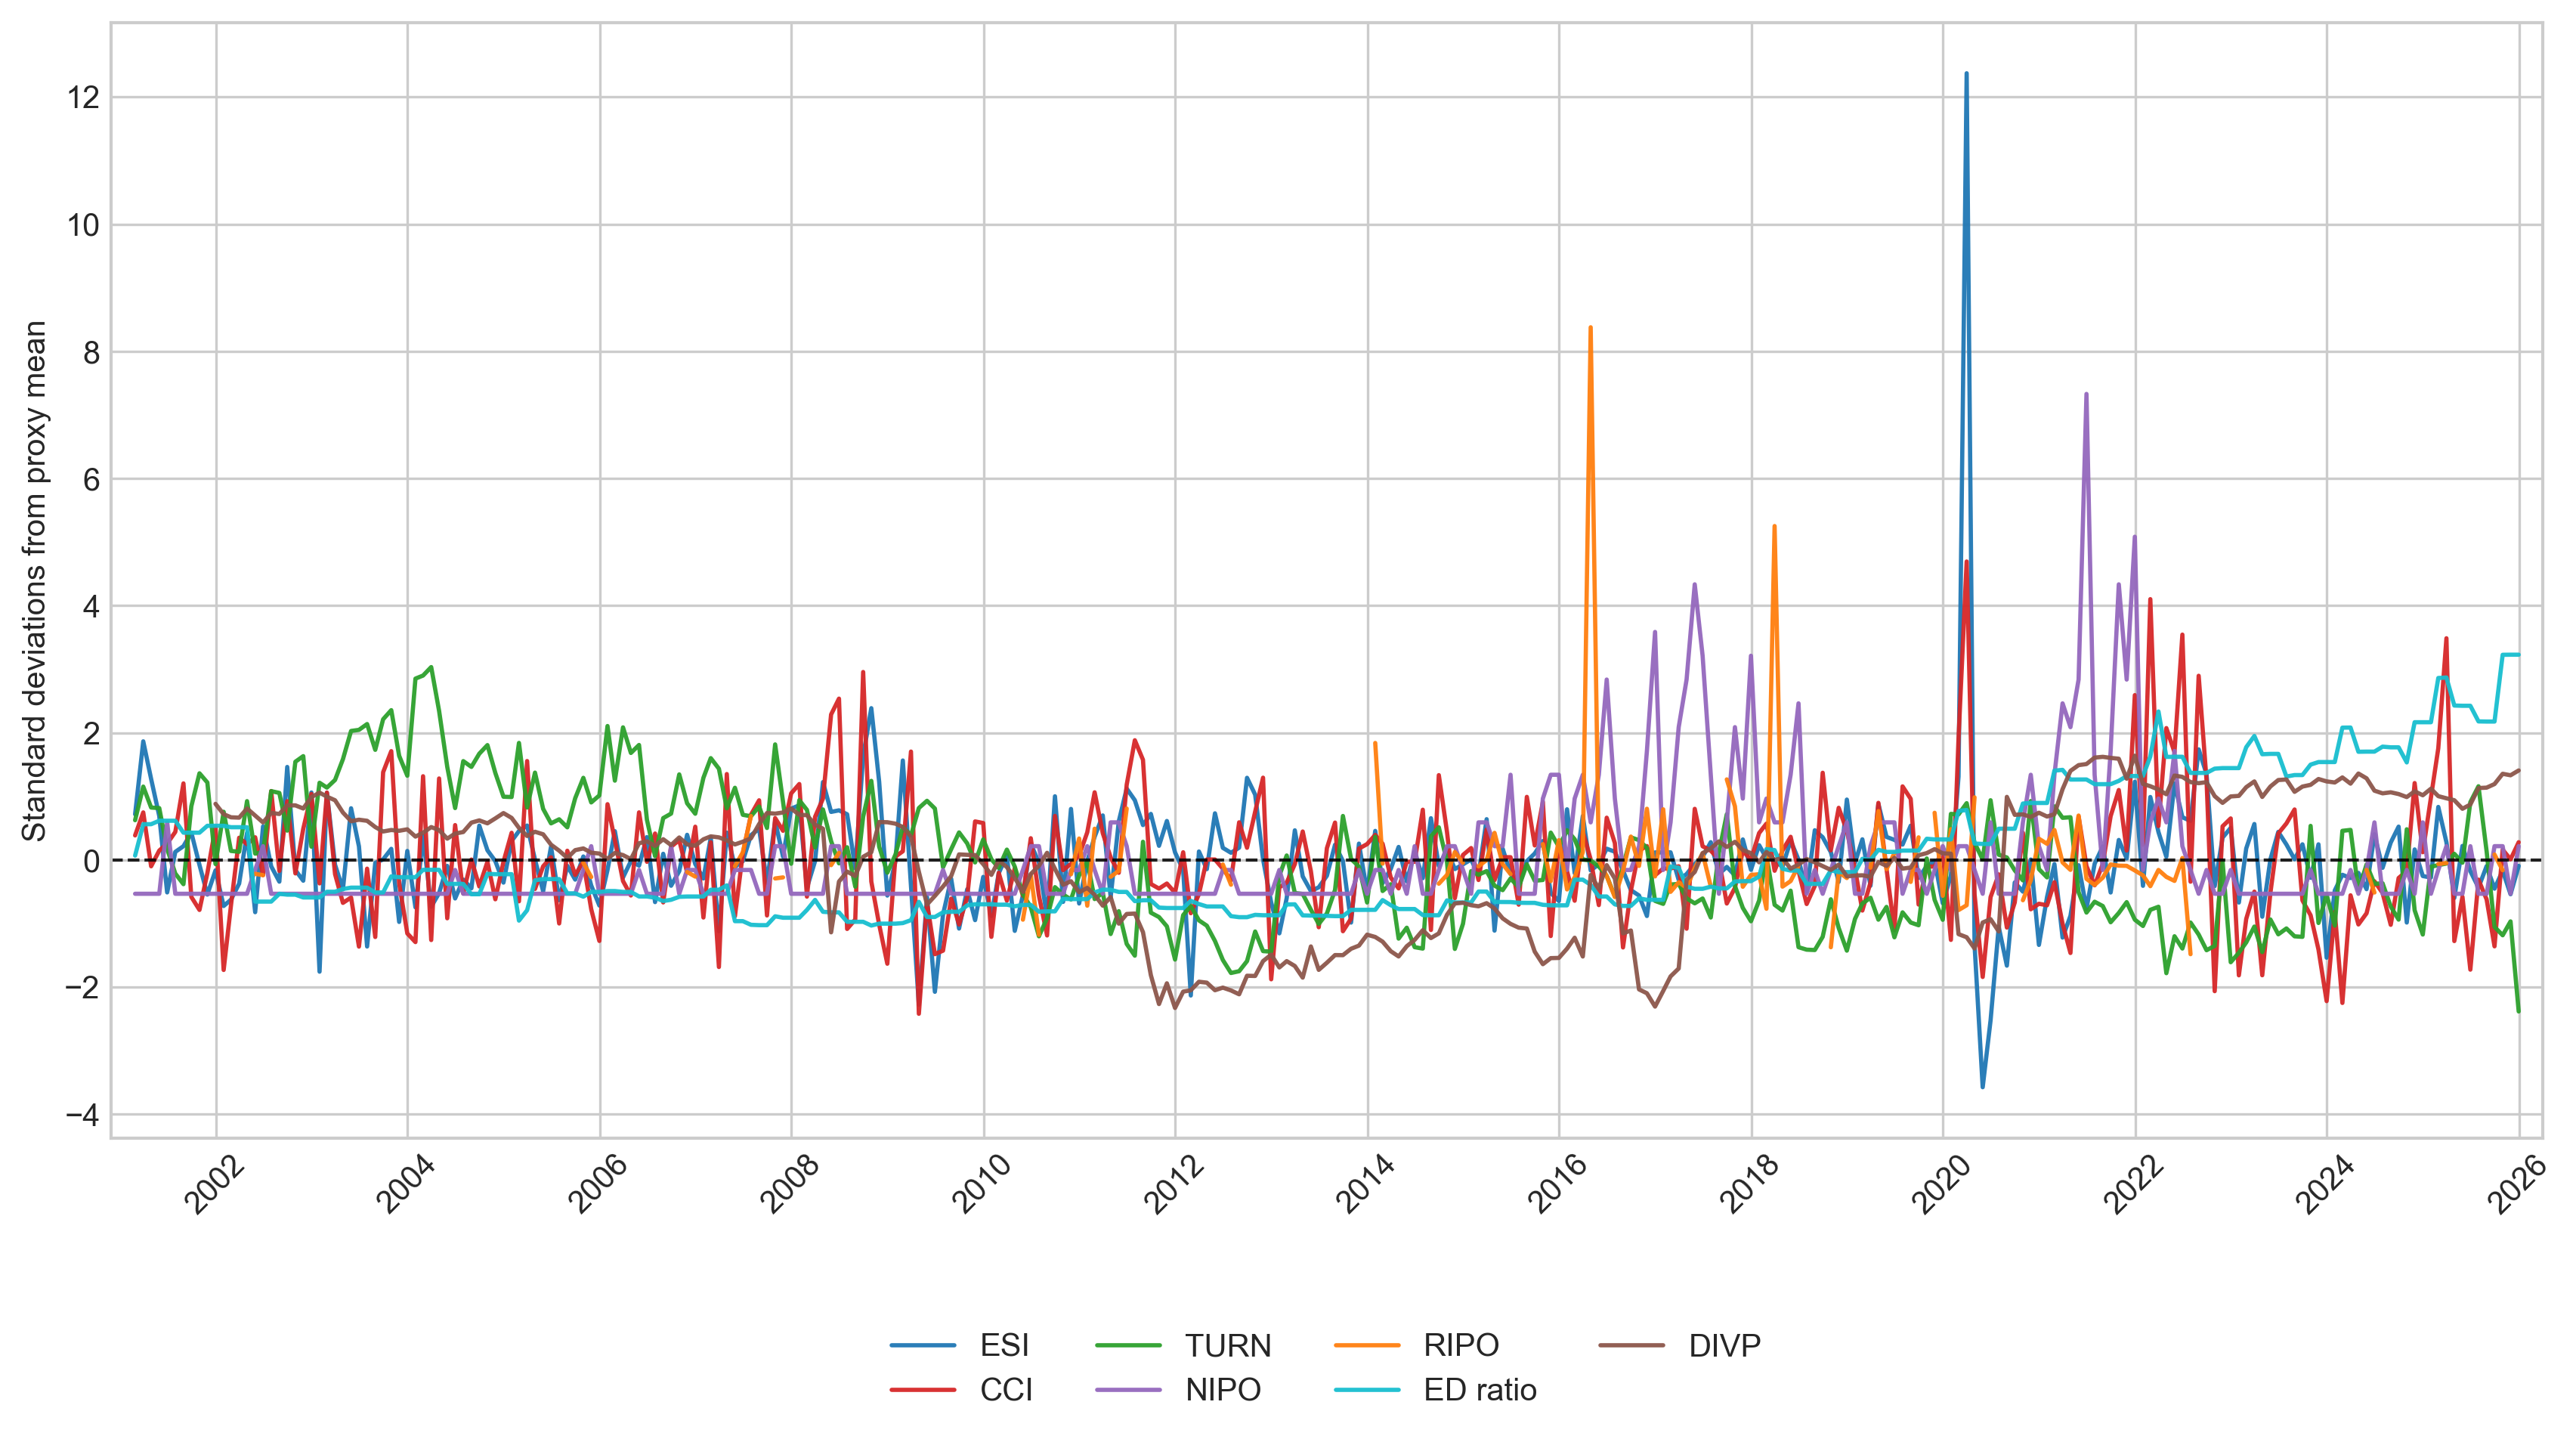
\includegraphics[width=\textwidth]{outputs/final_sentiment_sweden/final_standardized_sentiment_proxies_over_time.png}
    \caption{standardised sentiment proxy inputs over time}
    \label{fig:appendix_standardised_sentiment_proxies}
    \figurenote{Each proxy is standardised by subtracting its sample mean and dividing by its sample standard deviation. The horizontal dashed line marks zero. \var{RIPO_t} is plotted only in months with observed IPO initial-return information.}
\end{figure}


\begin{figure}[H]
    \centering
    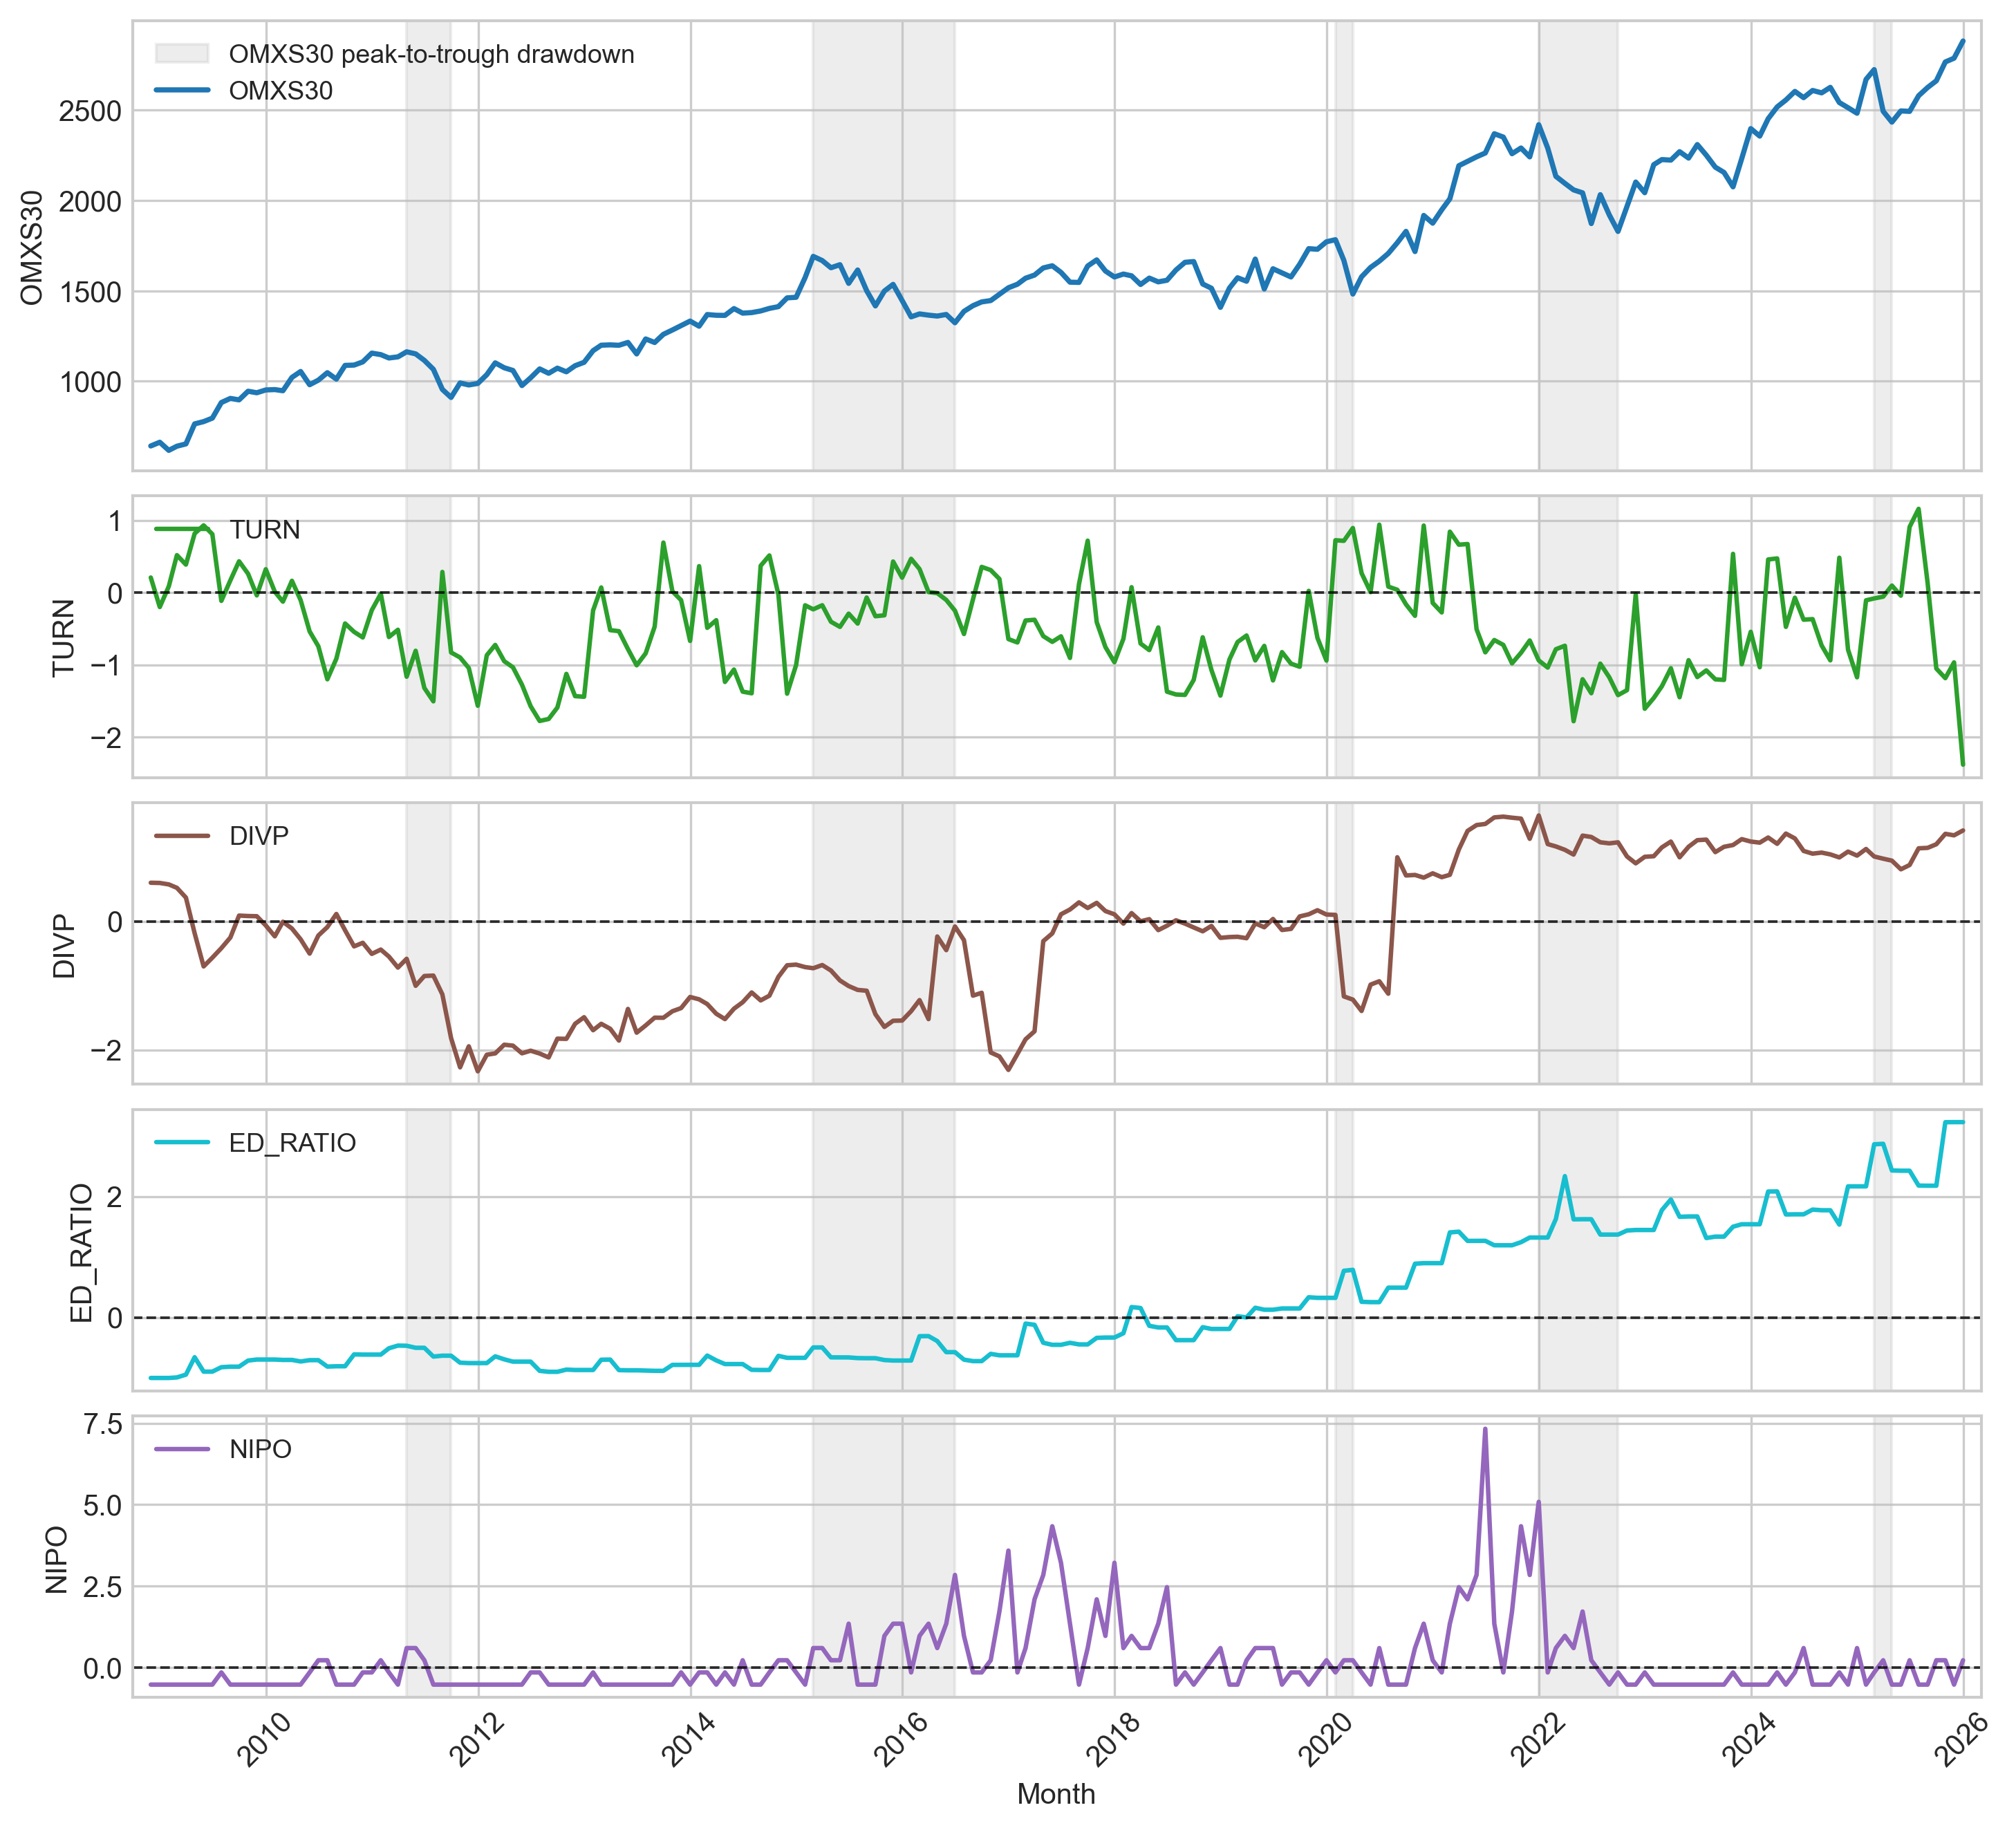
\includegraphics[width=\textwidth]{outputs/final_sentiment_sweden/final_omxs30_selected_standardized_proxy_drawdown_panels.png}
    \caption{OMXS30 drawdowns and selected standardised sentiment proxies}
    \label{fig:appendix_omxs30_proxy_drawdown_panels}
    \figurenote{Grey areas mark the five largest peak-to-trough OMXS30 drawdowns in the monthly OMXS30 series. Proxy series are standardised by subtracting each proxy mean and dividing by its sample standard deviation. The horizontal dashed line in each proxy panel marks zero.}
\end{figure}


\subsection{Appendix: Empirical findings}

\begin{table}[H]
    \centering
    \caption{Correlations of directional portfolio spreads}
    \label{tab:spread_correlations}
    \scriptsize
    \setlength{\tabcolsep}{2pt}
    \resizebox{\textwidth}{!}{%
    \begin{tabular}{lrrrrrrrrrrr}
        \toprule
        & ME & Age & Risk & Non-payer & Unprof. & PPE/A & GS & IVOL FF3 & ILLIQ & XTURN & E+BE \\
        \midrule
        ME & 1.00 &  &  &  &  &  &  &  &  &  &  \\
        Age & 0.11 & 1.00 &  &  &  &  &  &  &  &  &  \\
        Risk & 0.51 & -0.05 & 1.00 &  &  &  &  &  &  &  &  \\
        Non-payer & 0.70 & 0.16 & 0.61 & 1.00 &  &  &  &  &  &  &  \\
        Unprof. & 0.39 & 0.18 & 0.15 & 0.40 & 1.00 &  &  &  &  &  &  \\
        PPE/A & 0.26 & 0.02 & 0.27 & 0.22 & 0.13 & 1.00 &  &  &  &  &  \\
        GS & -0.04 & 0.09 & 0.05 & -0.06 & -0.13 & -0.09 & 1.00 &  &  &  &  \\
        IVOL FF3 & 0.62 & -0.04 & 0.81 & 0.65 & 0.20 & 0.20 & 0.03 & 1.00 &  &  &  \\
        ILLIQ & 0.81 & 0.14 & 0.45 & 0.66 & 0.32 & 0.19 & -0.06 & 0.59 & 1.00 &  &  \\
        XTURN & -0.28 & 0.21 & -0.56 & -0.47 & -0.13 & -0.22 & 0.07 & -0.54 & -0.07 & 1.00 &  \\
        E+BE & 0.17 & 0.02 & -0.01 & 0.18 & 0.81 & 0.08 & -0.12 & 0.02 & 0.11 & -0.03 & 1.00 \\
        \bottomrule
    \end{tabular}}
    \tablenote{The table reports pairwise correlations of monthly directional spread returns. Pairwise monthly observations range from 262 to 311.}
\end{table}

\begin{figure}[H]
    \centering
    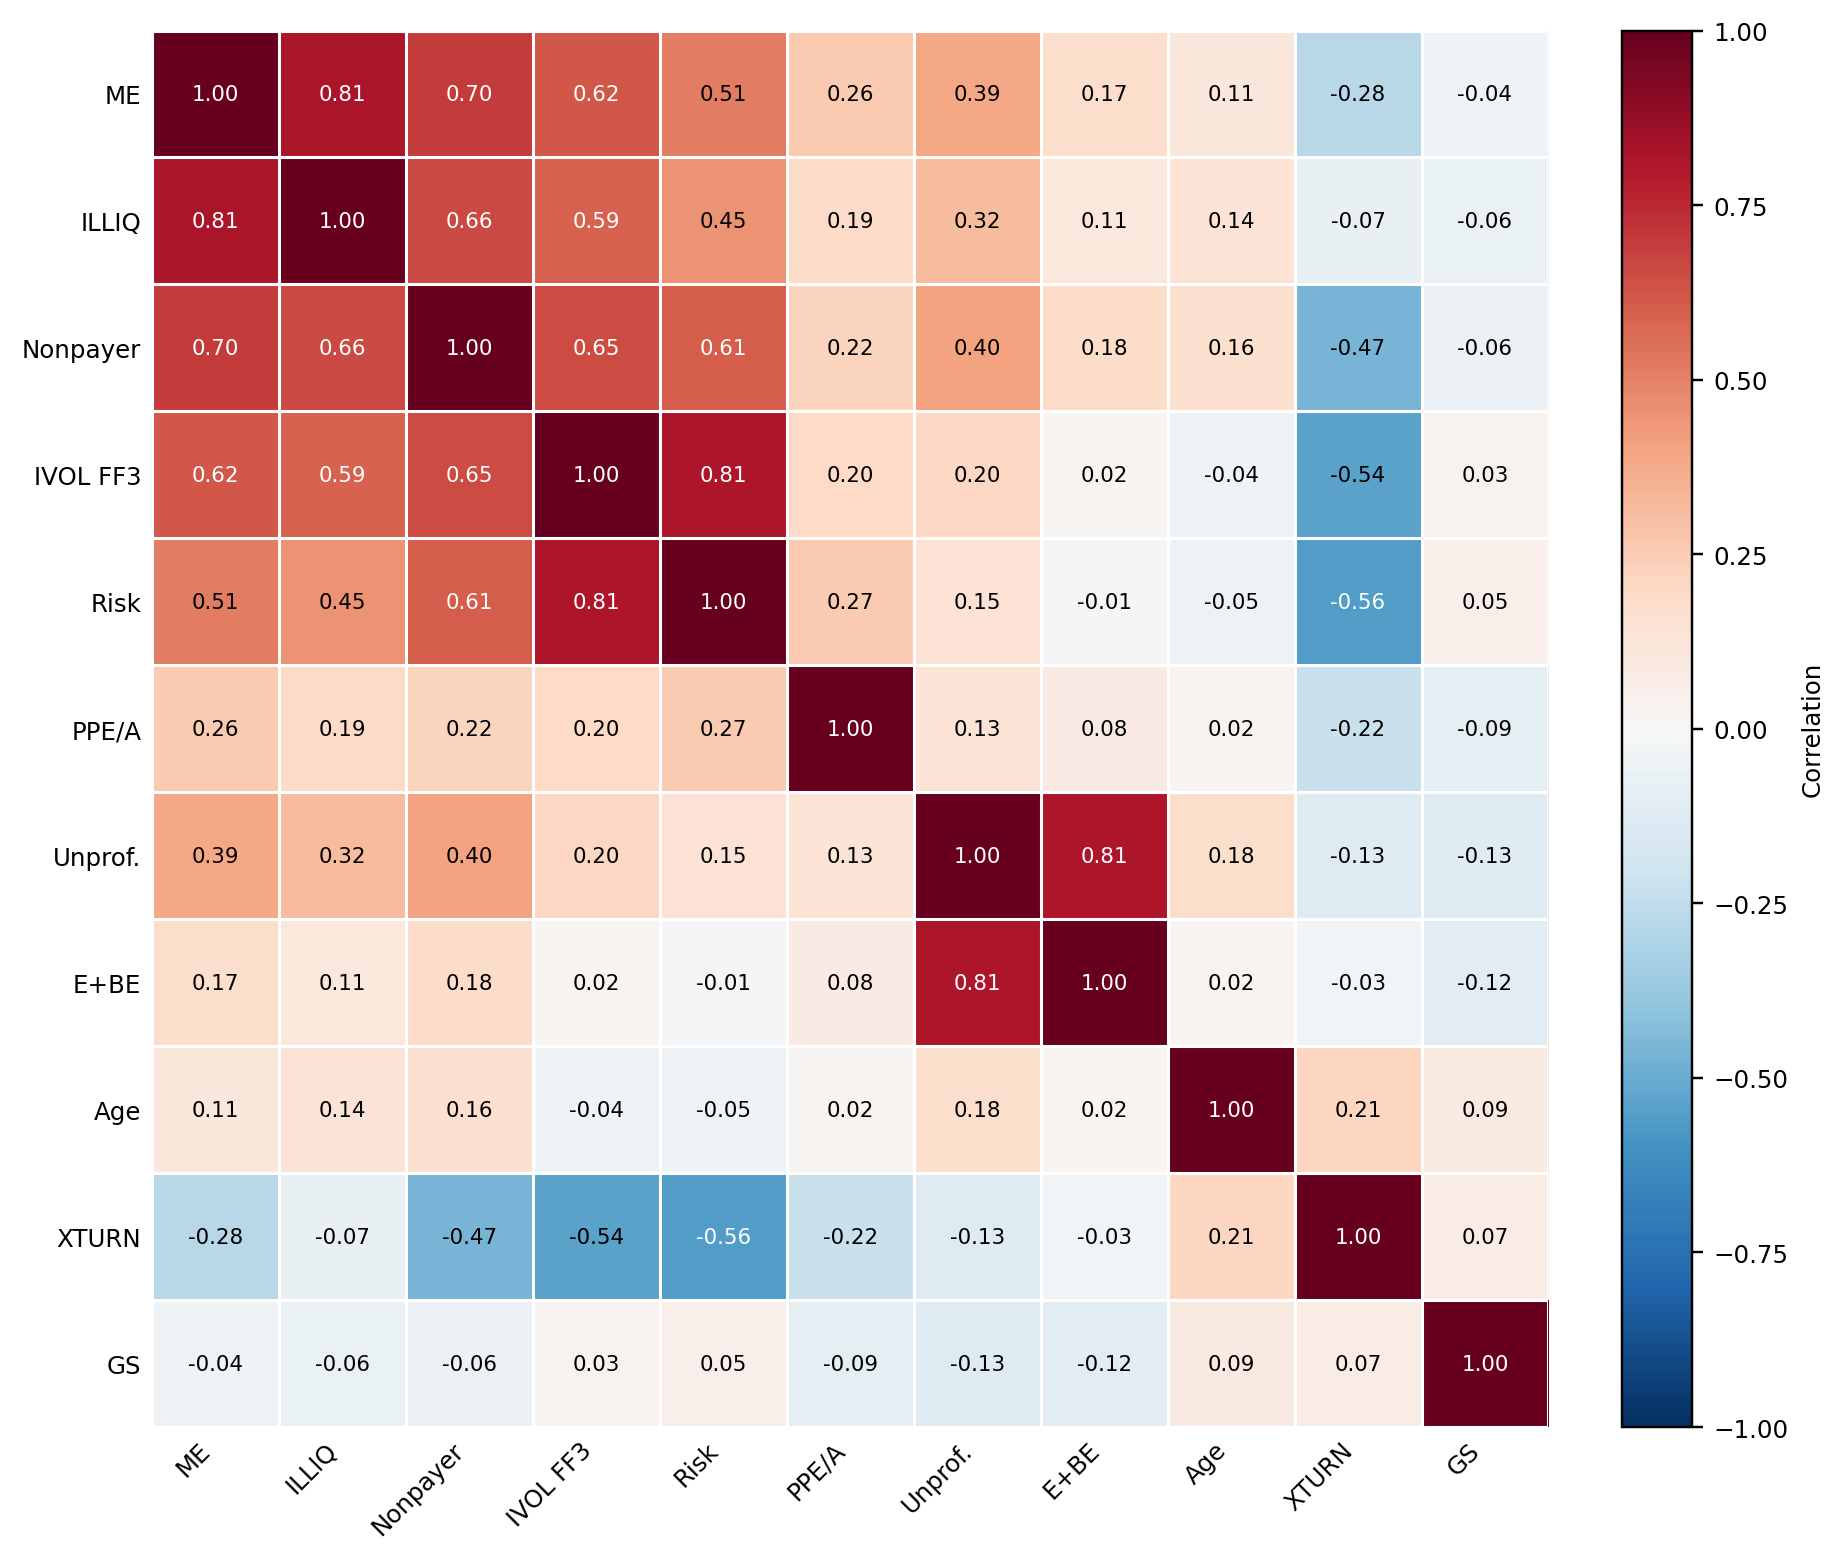
\includegraphics[width=0.85\textwidth]{outputs/final_sentiment_sweden/final_directional_spread_correlation_heatmap.png}
    \caption{Correlation heatmap of directional spread returns}
    \label{fig:spread_correlation_heatmap}
    \figurenote{The figure uses the same pairwise monthly directional-spread correlations as in \cref{tab:spread_correlations}. Characteristics are ordered by a deterministic nearest-correlation path so that related spread-return patterns appear next to each other.}
\end{figure}

\begin{table}[H]
    \centering
    \caption{Predictive regression summary by return horizon}
    \label{tab:results_by_horizon}
    \small
    \begin{tabular}{llllllr}
        \toprule
        Horizon & Index & Mean coef. & Mean HAC t & Expected t & Bootstrap t & 5\% share \\
        \midrule
        1 & Orthogonalised & -0.97 & -1.62 & 1.62 & 1.62 & 0.36 \\
        1 & Raw & -0.59 & -0.94 & 0.94 & 0.86 & 0.27 \\
        3 & Orthogonalised & -2.04 & -1.46 & 1.46 & 1.45 & 0.36 \\
        3 & Raw & -1.03 & -0.63 & 0.63 & 0.61 & 0.18 \\
        6 & Orthogonalised & -4.37\textsuperscript{*} & -1.93 & 1.93 & 1.91 & 0.45 \\
        6 & Raw & -2.63 & -1.17 & 1.17 & 1.11 & 0.09 \\
        12 & Orthogonalised & -7.89\textsuperscript{**} & -2.22 & 2.22 & 2.08 & 0.64 \\
        12 & Raw & -4.00 & -1.06 & 1.06 & 1.00 & 0.09 \\
        \bottomrule
    \end{tabular}
    \tablenote{The expected-signed t-statistic multiplies the coefficient t-statistic by the theoretically expected sign. Positive values support the sentiment-reversal hypothesis. Stars on mean coefficients are based on the absolute mean HAC t-statistic and are descriptive for horizon-level averages.}
\end{table}


The detailed horizon tables place \var{SENT} and \var{SENT^{\perp}} side by side. The \var{SENT^{\perp}} estimates across all horizons appear in \cref{tab:sent_orth_predictive_overview}.


\begin{table}[!htbp]
\centering
\caption{Predictive Regressions for Directional Sentiment-Prone Spreads: 1-Month Horizon}
\label{tab:bw2006_horizon_1m}
\small
\begin{tabularx}{\textwidth}{lXlllll}
\toprule
Characteristic & Spread & \multicolumn{2}{c}{\var{SENT}} & \multicolumn{3}{c}{\var{SENT^{\perp}}} \\
\cmidrule(lr){3-4}\cmidrule(lr){5-7}
 & & Coef. & HAC $t$ & Coef. & HAC $t$ & Boot. $t$ \\
\midrule
\multicolumn{7}{l}{\textit{Panel A. Size, Age, and Risk}} \\
\var{ME} & Small minus big & -0.92 & -1.17 & -1.34\textsuperscript{*} & -1.90 & -1.92 \\
\var{Age} & Young minus old & -0.40 & -0.91 & -0.38 & -0.80 & -0.83 \\
$\sigma$ & High minus low & -0.79 & -1.19 & -2.60\textsuperscript{***} & -3.50 & -3.51 \\
\var{IVOL^{FF3}} & High minus low & -0.68 & -0.85 & -2.24\textsuperscript{***} & -2.69 & -2.69 \\
\midrule
\multicolumn{7}{l}{\textit{Panel B. Profitability and Dividend Policy}} \\
\var{E+BE} & Low minus high & 0.28 & 0.58 & -0.44 & -0.64 & -0.62 \\
\var{Unprofitable} & Unprofitable minus profitable & -0.03 & -0.08 & -0.54 & -0.96 & -0.98 \\
\var{Nonpayer} & Nonpayer minus payer & 0.07 & 0.27 & -0.63\textsuperscript{**} & -2.24 & -2.26 \\
\midrule
\multicolumn{7}{l}{\textit{Panel C. Tangibility and Growth Opportunities}} \\
\var{PPE/A} & Low minus high & -1.37\textsuperscript{**} & -2.41 & -1.27\textsuperscript{***} & -2.99 & -2.94 \\
\var{GS} & High minus low & -1.10\textsuperscript{**} & -2.18 & -0.80 & -1.33 & -1.28 \\
\midrule
\multicolumn{7}{l}{\textit{Panel D. Trading Frictions}} \\
\var{ILLIQ} & High minus low & 0.10 & 0.20 & -0.30 & -0.67 & -0.66 \\
\var{XTURN} & Low minus high & -1.68\textsuperscript{**} & -2.56 & -0.11 & -0.16 & -0.16 \\
\bottomrule
\end{tabularx}
\tablenote{Each row reports the coefficient on lagged sentiment in a factor-adjusted predictive regression of the directional spread return on sentiment and contemporaneous factor returns. For continuous characteristics, directional spreads use the sentiment-prone extreme decile minus the opposite extreme decile; binary spreads use the two natural groups. Negative coefficients are theory-consistent because high sentiment predicts lower subsequent returns for the sentiment-prone side. Coefficient stars mark HAC significance at 10\%, 5\%, and 1\%.}
\end{table}


\begin{table}[!htbp]
\centering
\caption{Predictive Regressions for Directional Sentiment-Prone Spreads: 3-Month Horizon}
\label{tab:bw2006_horizon_3m}
\small
\begin{tabularx}{\textwidth}{lXlllll}
\toprule
Characteristic & Spread & \multicolumn{2}{c}{\var{SENT}} & \multicolumn{3}{c}{\var{SENT^{\perp}}} \\
\cmidrule(lr){3-4}\cmidrule(lr){5-7}
 & & Coef. & HAC $t$ & Coef. & HAC $t$ & Boot. $t$ \\
\midrule
\multicolumn{7}{l}{\textit{Panel A. Size, Age, and Risk}} \\
\var{ME} & Small minus big & -0.52 & -0.34 & -2.44 & -1.38 & -1.39 \\
\var{Age} & Young minus old & -1.53 & -1.35 & -1.06 & -0.79 & -0.74 \\
$\sigma$ & High minus low & -1.30 & -0.81 & -6.49\textsuperscript{***} & -3.56 & -3.48 \\
\var{IVOL^{FF3}} & High minus low & -1.53 & -0.85 & -5.60\textsuperscript{***} & -2.97 & -3.01 \\
\midrule
\multicolumn{7}{l}{\textit{Panel B. Profitability and Dividend Policy}} \\
\var{E+BE} & Low minus high & 1.06 & 1.25 & 0.43 & 0.34 & 0.32 \\
\var{Unprofitable} & Unprofitable minus profitable & 0.41 & 0.75 & -1.11 & -1.36 & -1.36 \\
\var{Nonpayer} & Nonpayer minus payer & 0.19 & 0.32 & -1.88\textsuperscript{**} & -2.46 & -2.48 \\
\midrule
\multicolumn{7}{l}{\textit{Panel C. Tangibility and Growth Opportunities}} \\
\var{PPE/A} & Low minus high & -3.47\textsuperscript{***} & -2.85 & -4.46\textsuperscript{***} & -3.86 & -3.79 \\
\var{GS} & High minus low & -1.88 & -1.58 & -0.88 & -0.64 & -0.63 \\
\midrule
\multicolumn{7}{l}{\textit{Panel D. Trading Frictions}} \\
\var{ILLIQ} & High minus low & 0.72 & 0.85 & -0.03 & -0.03 & -0.03 \\
\var{XTURN} & Low minus high & -3.48\textsuperscript{**} & -2.30 & 1.04 & 0.62 & 0.63 \\
\bottomrule
\end{tabularx}
\tablenote{Each row reports the coefficient on lagged sentiment in a factor-adjusted predictive regression of the directional spread return on sentiment and contemporaneous factor returns. For continuous characteristics, directional spreads use the sentiment-prone extreme decile minus the opposite extreme decile; binary spreads use the two natural groups. Negative coefficients are theory-consistent because high sentiment predicts lower subsequent returns for the sentiment-prone side. Coefficient stars mark HAC significance at 10\%, 5\%, and 1\%.}
\end{table}


\begin{table}[!htbp]
\centering
\caption{Predictive Regressions for Directional Sentiment-Prone Spreads: 6-Month Horizon}
\label{tab:bw2006_horizon_6m}
\small
\begin{tabularx}{\textwidth}{lXlllll}
\toprule
Characteristic & Spread & \multicolumn{2}{c}{\var{SENT}} & \multicolumn{3}{c}{\var{SENT^{\perp}}} \\
\cmidrule(lr){3-4}\cmidrule(lr){5-7}
 & & Coef. & HAC $t$ & Coef. & HAC $t$ & Boot. $t$ \\
\midrule
\multicolumn{7}{l}{\textit{Panel A. Size, Age, and Risk}} \\
\var{ME} & Small minus big & -3.82 & -1.41 & -6.55\textsuperscript{**} & -2.39 & -2.39 \\
\var{Age} & Young minus old & -3.28\textsuperscript{*} & -1.87 & -2.86 & -1.23 & -1.22 \\
$\sigma$ & High minus low & -4.22\textsuperscript{*} & -1.65 & -12.08\textsuperscript{***} & -4.30 & -4.25 \\
\var{IVOL^{FF3}} & High minus low & -3.82 & -1.36 & -11.74\textsuperscript{***} & -4.05 & -4.02 \\
\midrule
\multicolumn{7}{l}{\textit{Panel B. Profitability and Dividend Policy}} \\
\var{E+BE} & Low minus high & 0.98 & 0.63 & 0.41 & 0.18 & 0.18 \\
\var{Unprofitable} & Unprofitable minus profitable & 0.04 & 0.04 & -2.50\textsuperscript{*} & -1.84 & -1.76 \\
\var{Nonpayer} & Nonpayer minus payer & -0.14 & -0.14 & -3.58\textsuperscript{***} & -2.88 & -2.91 \\
\midrule
\multicolumn{7}{l}{\textit{Panel C. Tangibility and Growth Opportunities}} \\
\var{PPE/A} & Low minus high & -6.02\textsuperscript{***} & -3.40 & -8.34\textsuperscript{***} & -4.21 & -4.11 \\
\var{GS} & High minus low & -3.70\textsuperscript{*} & -1.77 & -1.41 & -0.55 & -0.54 \\
\midrule
\multicolumn{7}{l}{\textit{Panel D. Trading Frictions}} \\
\var{ILLIQ} & High minus low & -0.20 & -0.15 & -1.32 & -0.65 & -0.64 \\
\var{XTURN} & Low minus high & -4.77\textsuperscript{*} & -1.76 & 1.91 & 0.67 & 0.69 \\
\bottomrule
\end{tabularx}
\tablenote{Each row reports the coefficient on lagged sentiment in a factor-adjusted predictive regression of the directional spread return on sentiment and contemporaneous factor returns. For continuous characteristics, directional spreads use the sentiment-prone extreme decile minus the opposite extreme decile; binary spreads use the two natural groups. Negative coefficients are theory-consistent because high sentiment predicts lower subsequent returns for the sentiment-prone side. Coefficient stars mark HAC significance at 10\%, 5\%, and 1\%.}
\end{table}


\begin{table}[!htbp]
\centering
\caption{Predictive Regressions for Directional Sentiment-Prone Spreads: 12-Month Horizon}
\label{tab:bw2006_horizon_12m}
\small
\begin{tabularx}{\textwidth}{lXlllll}
\toprule
Characteristic & Spread & \multicolumn{2}{c}{\var{SENT}} & \multicolumn{3}{c}{\var{SENT^{\perp}}} \\
\cmidrule(lr){3-4}\cmidrule(lr){5-7}
 & & Coef. & HAC $t$ & Coef. & HAC $t$ & Boot. $t$ \\
\midrule
\multicolumn{7}{l}{\textit{Panel A. Size, Age, and Risk}} \\
\var{ME} & Small minus big & -9.14 & -1.61 & -14.04\textsuperscript{***} & -3.15 & -2.84 \\
\var{Age} & Young minus old & -6.33\textsuperscript{*} & -1.82 & -8.37\textsuperscript{**} & -2.29 & -2.11 \\
$\sigma$ & High minus low & -5.45 & -1.09 & -19.65\textsuperscript{***} & -4.43 & -4.18 \\
\var{IVOL^{FF3}} & High minus low & -5.15 & -1.07 & -18.42\textsuperscript{***} & -3.75 & -3.76 \\
\midrule
\multicolumn{7}{l}{\textit{Panel B. Profitability and Dividend Policy}} \\
\var{E+BE} & Low minus high & 2.08 & 0.92 & 0.08 & 0.02 & 0.02 \\
\var{Unprofitable} & Unprofitable minus profitable & -0.99 & -0.89 & -4.86\textsuperscript{***} & -3.04 & -2.90 \\
\var{Nonpayer} & Nonpayer minus payer & -0.66 & -0.41 & -4.96\textsuperscript{***} & -2.80 & -2.59 \\
\midrule
\multicolumn{7}{l}{\textit{Panel C. Tangibility and Growth Opportunities}} \\
\var{PPE/A} & Low minus high & -11.44\textsuperscript{***} & -3.19 & -15.27\textsuperscript{***} & -4.83 & -4.37 \\
\var{GS} & High minus low & -3.88 & -1.37 & -3.21 & -0.61 & -0.58 \\
\midrule
\multicolumn{7}{l}{\textit{Panel D. Trading Frictions}} \\
\var{ILLIQ} & High minus low & -0.13 & -0.05 & -2.58 & -0.72 & -0.69 \\
\var{XTURN} & Low minus high & -2.85 & -1.10 & 4.46 & 1.23 & 1.14 \\
\bottomrule
\end{tabularx}
\tablenote{Each row reports the coefficient on lagged sentiment in a factor-adjusted predictive regression of the directional spread return on sentiment and contemporaneous factor returns. For continuous characteristics, directional spreads use the sentiment-prone extreme decile minus the opposite extreme decile; binary spreads use the two natural groups. Negative coefficients are theory-consistent because high sentiment predicts lower subsequent returns for the sentiment-prone side. Coefficient stars mark HAC significance at 10\%, 5\%, and 1\%.}
\end{table}


\subsection{Appendix: Discussion}

\subsubsection{Empirical Consequences}


The Covid-winsorised appendix check modifies only the Sibley-expanded robustness index. \var{SENT^{\perp}} remains the unadjusted series because the Covid shock is treated as an economically real sentiment episode rather than as a data error. \var{SENT^{\perp}} changes little after the Covid adjustment, while \var{SENT^{S}} is materially affected by the crisis-period proxy adjustment.


\begin{figure}[H]
    \centering
    \includegraphics[width=\textwidth]{outputs/sentiment_outlier_experiment_sweden/experiment_sentiment_original_vs_adjusted_over_time.png}
    \caption{Original and Covid-winsorised sentiment indices}
    \label{fig:appendix_covid_winsorised_sentiment_indices}
    \figurenote{The Covid-winsorised series cap extreme March--April 2020 raw proxy observations before PCA construction. The adjustment is triggered by the March 2020 \var{ESI_t} and \var{CCI_t} observations. The baseline \var{SENT^{\perp}} series remains close to the original series, while \var{SENT^{S}} changes materially.}
\end{figure}

\subsubsection{Sibley-Expanded Sentiment Robustness}


The Sibley-expanded comparison reports the coefficient and HAC t-statistic for each directional-spread regression under \var{SENT^{\perp}} and \var{SENT^{S}}. The comparison column classifies each characteristic-horizon test by whether the expected negative coefficient is significant at the 5\% HAC level before and after the Sibley-expanded macro adjustment. Negative coefficients support the expected sentiment-reversal pattern because each spread is coded as sentiment-prone minus sentiment-insensitive.


\begin{table}[H]
\centering
\caption{Sibley-expanded sentiment robustness by characteristic and horizon}
\label{tab:appendix_sibley_characteristic_horizon}
\scriptsize
\begin{tabularx}{\textwidth}{>{\raggedright\arraybackslash}X>{\raggedright\arraybackslash}p{0.075\textwidth}>{\raggedleft\arraybackslash}p{0.065\textwidth}>{\raggedright\arraybackslash}p{0.075\textwidth}>{\raggedleft\arraybackslash}p{0.065\textwidth}>{\raggedright\arraybackslash}p{0.18\textwidth}}
\toprule
Characteristic & \multicolumn{2}{c}{\var{SENT^{\perp}}} & \multicolumn{2}{c}{\var{SENT^{S}}} & Baseline $\rightarrow$ Sibley \\
\cmidrule(lr){2-3} \cmidrule(lr){4-5}
 & Coef. & HAC \var{t} & Coef. & HAC \var{t} &  \\
\midrule
\multicolumn{6}{l}{\textit{1-month horizon}}\\
Small firms & -1.34\textsuperscript{*} & -1.90 & -0.79 & -1.09 & Never 5\% \\
Young firms & -0.38 & -0.80 & -0.07 & -0.17 & Never 5\% \\
\textbf{Total risk} & \textbf{-2.60\textsuperscript{***}} & \textbf{-3.50} & \textbf{-1.14} & \textbf{-1.64} & \textbf{Loses 5\%} \\
\textbf{\var{IVOL^{FF3}}} & \textbf{-2.24\textsuperscript{***}} & \textbf{-2.69} & \textbf{-0.62} & \textbf{-0.81} & \textbf{Loses 5\%} \\
Low profitability & -0.44 & -0.64 & 0.24 & 0.44 & Never 5\% \\
Unprofitable & -0.54 & -0.96 & -0.15 & -0.34 & Never 5\% \\
\textbf{Non-dividend payer} & \textbf{-0.63\textsuperscript{**}} & \textbf{-2.24} & \textbf{0.07} & \textbf{0.38} & \textbf{Loses 5\%} \\
Low tangibility & -1.27\textsuperscript{***} & -2.99 & -1.55\textsuperscript{**} & -2.50 & Stays 5\% \\
Sales growth & -0.80 & -1.33 & -0.53 & -0.97 & Never 5\% \\
Illiquidity & -0.30 & -0.67 & 0.15 & 0.31 & Never 5\% \\
Low turnover & -0.11 & -0.16 & -1.08\textsuperscript{*} & -1.86 & Never 5\% \\
\midrule
\multicolumn{6}{l}{\textit{3-month horizon}}\\
Small firms & -2.44 & -1.38 & 0.01 & 0.01 & Never 5\% \\
Young firms & -1.06 & -0.79 & -0.46 & -0.48 & Never 5\% \\
\textbf{Total risk} & \textbf{-6.49\textsuperscript{***}} & \textbf{-3.56} & \textbf{-1.30} & \textbf{-0.96} & \textbf{Loses 5\%} \\
\textbf{\var{IVOL^{FF3}}} & \textbf{-5.60\textsuperscript{***}} & \textbf{-2.97} & \textbf{-0.63} & \textbf{-0.41} & \textbf{Loses 5\%} \\
Low profitability & 0.43 & 0.34 & 1.23 & 1.43 & Never 5\% \\
Unprofitable & -1.11 & -1.36 & 0.48 & 1.22 & Never 5\% \\
\textbf{Non-dividend payer} & \textbf{-1.88\textsuperscript{**}} & \textbf{-2.46} & \textbf{0.30} & \textbf{0.74} & \textbf{Loses 5\%} \\
Low tangibility & -4.46\textsuperscript{***} & -3.86 & -3.11\textsuperscript{***} & -2.88 & Stays 5\% \\
Sales growth & -0.88 & -0.64 & -0.90 & -0.98 & Never 5\% \\
Illiquidity & -0.03 & -0.03 & 0.76 & 1.12 & Never 5\% \\
Low turnover & 1.04 & 0.62 & -1.82 & -1.45 & Never 5\% \\
\midrule
\multicolumn{6}{l}{\textit{6-month horizon}}\\
\textbf{Small firms} & \textbf{-6.55\textsuperscript{**}} & \textbf{-2.39} & \textbf{-3.03} & \textbf{-1.27} & \textbf{Loses 5\%} \\
Young firms & -2.86 & -1.23 & -0.54 & -0.39 & Never 5\% \\
\textbf{Total risk} & \textbf{-12.08\textsuperscript{***}} & \textbf{-4.30} & \textbf{-3.29} & \textbf{-1.62} & \textbf{Loses 5\%} \\
\textbf{\var{IVOL^{FF3}}} & \textbf{-11.74\textsuperscript{***}} & \textbf{-4.05} & \textbf{-1.44} & \textbf{-0.72} & \textbf{Loses 5\%} \\
Low profitability & 0.41 & 0.18 & 1.62 & 0.97 & Never 5\% \\
Unprofitable & -2.50\textsuperscript{*} & -1.84 & 0.17 & 0.26 & Never 5\% \\
\textbf{Non-dividend payer} & \textbf{-3.58\textsuperscript{***}} & \textbf{-2.88} & \textbf{-0.20} & \textbf{-0.28} & \textbf{Loses 5\%} \\
Low tangibility & -8.34\textsuperscript{***} & -4.21 & -4.96\textsuperscript{***} & -3.10 & Stays 5\% \\
Sales growth & -1.41 & -0.55 & -1.62 & -1.11 & Never 5\% \\
Illiquidity & -1.32 & -0.65 & -0.16 & -0.15 & Never 5\% \\
Low turnover & 1.91 & 0.67 & -2.67 & -1.25 & Never 5\% \\
\midrule
\multicolumn{6}{l}{\textit{12-month horizon}}\\
\textbf{Small firms} & \textbf{-14.04\textsuperscript{***}} & \textbf{-3.15} & \textbf{-6.64} & \textbf{-1.46} & \textbf{Loses 5\%} \\
\textbf{Young firms} & \textbf{-8.37\textsuperscript{**}} & \textbf{-2.29} & \textbf{-1.18} & \textbf{-0.52} & \textbf{Loses 5\%} \\
\textbf{Total risk} & \textbf{-19.65\textsuperscript{***}} & \textbf{-4.43} & \textbf{-1.63} & \textbf{-0.46} & \textbf{Loses 5\%} \\
\textbf{\var{IVOL^{FF3}}} & \textbf{-18.42\textsuperscript{***}} & \textbf{-3.75} & \textbf{0.59} & \textbf{0.22} & \textbf{Loses 5\%} \\
Low profitability & 0.08 & 0.02 & 1.27 & 0.70 & Never 5\% \\
\textbf{Unprofitable} & \textbf{-4.86\textsuperscript{***}} & \textbf{-3.04} & \textbf{-1.32} & \textbf{-1.50} & \textbf{Loses 5\%} \\
\textbf{Non-dividend payer} & \textbf{-4.96\textsuperscript{***}} & \textbf{-2.80} & \textbf{-1.39} & \textbf{-1.27} & \textbf{Loses 5\%} \\
Low tangibility & -15.27\textsuperscript{***} & -4.83 & -8.97\textsuperscript{***} & -3.11 & Stays 5\% \\
Sales growth & -3.21 & -0.61 & -2.49 & -1.24 & Never 5\% \\
Illiquidity & -2.58 & -0.72 & 1.09 & 0.62 & Never 5\% \\
Low turnover & 4.46 & 1.23 & -0.03 & -0.01 & Never 5\% \\
\bottomrule
\end{tabularx}
\tablenote{Coefficients are percentage-point effects on future directional-spread returns. HAC t-statistics use the Newey-West standard errors from the predictive regressions. ``Baseline $\rightarrow$ Sibley'' classifies theory-consistent 5\% HAC significance when moving from \var{SENT^{\perp}} to \var{SENT^{S}}. Coefficient stars mark HAC significance at 10\%, 5\%, and 1\%. Bold rows identify cases where significance is lost under the Sibley-expanded index.}
\end{table}

The Covid-winsorised Sibley-expanded index stays significant in 4 characteristic-horizon tests, gains significance in 11, and is never significant in 29 relative to the unadjusted Sibley-expanded index. Relative to \var{SENT^{\perp}}, 12 tests stay significant, 8 lose significance, 3 gain significance, and 21 are never significant. The adjustment makes the Sibley-expanded index more predictive in several rows, especially at longer horizons, but it does not fully reproduce the \var{SENT^{\perp}} cross-sectional pattern.


{\scriptsize
\setlength{\tabcolsep}{3pt}
\renewcommand{\arraystretch}{0.94}
\begin{longtable}{@{}>{\raggedright\arraybackslash}p{0.18\textwidth}>{\raggedright\arraybackslash}p{0.075\textwidth}>{\raggedleft\arraybackslash}p{0.06\textwidth}>{\raggedright\arraybackslash}p{0.075\textwidth}>{\raggedleft\arraybackslash}p{0.06\textwidth}>{\raggedright\arraybackslash}p{0.15\textwidth}>{\raggedright\arraybackslash}p{0.17\textwidth}@{}}
\caption{Covid-winsorised Sibley-expanded sentiment regressions by characteristic and horizon}\label{tab:appendix_covid_winsorised_sibley_characteristic_horizon}\\
\toprule
Characteristic & \multicolumn{2}{c}{\var{SENT^{S}}} & \multicolumn{2}{c}{\var{SENT^{S,C}}} & Sibley $\rightarrow$ adj. & Baseline $\rightarrow$ adj. \\
\cmidrule(lr){2-3} \cmidrule(lr){4-5}
 & Coef. & HAC \var{t} & Coef. & HAC \var{t} & & \\
\midrule
\endfirsthead
\toprule
Characteristic & \multicolumn{2}{c}{\var{SENT^{S}}} & \multicolumn{2}{c}{\var{SENT^{S,C}}} & Sibley $\rightarrow$ adj. & Baseline $\rightarrow$ adj. \\
\cmidrule(lr){2-3} \cmidrule(lr){4-5}
 & Coef. & HAC \var{t} & Coef. & HAC \var{t} & & \\
\midrule
\endhead
\midrule
\multicolumn{7}{r}{\textit{Continued on next page}} \\
\endfoot
\bottomrule
\endlastfoot
\multicolumn{7}{l}{\textit{1-month horizon}}\\
Small firms & -0.79 & -1.09 & -1.29\textsuperscript{*} & -1.78 & Never 5\% & Never 5\% \\
Young firms & -0.07 & -0.17 & -0.25 & -0.48 & Never 5\% & Never 5\% \\
\textbf{Total risk} & \textbf{-1.14} & \textbf{-1.64} & \textbf{-1.36\textsuperscript{*}} & \textbf{-1.73} & \textbf{Never 5\%} & \textbf{Loses 5\%} \\
\textbf{\var{IVOL^{FF3}}} & \textbf{-0.62} & \textbf{-0.81} & \textbf{-1.50\textsuperscript{*}} & \textbf{-1.71} & \textbf{Never 5\%} & \textbf{Loses 5\%} \\
Low profitability & 0.24 & 0.44 & 0.43 & 1.05 & Never 5\% & Never 5\% \\
Unprofitable & -0.15 & -0.34 & 0.36 & 1.00 & Never 5\% & Never 5\% \\
\textbf{Non-dividend payer} & \textbf{0.07} & \textbf{0.38} & \textbf{-0.10} & \textbf{-0.30} & \textbf{Never 5\%} & \textbf{Loses 5\%} \\
Low tangibility & -1.55\textsuperscript{**} & -2.50 & -1.29\textsuperscript{***} & -2.95 & Stays 5\% & Stays 5\% \\
Sales growth & -0.53 & -0.97 & -1.10\textsuperscript{*} & -1.79 & Never 5\% & Never 5\% \\
Illiquidity & 0.15 & 0.31 & -0.09 & -0.19 & Never 5\% & Never 5\% \\
Low turnover & -1.08\textsuperscript{*} & -1.86 & -0.60 & -0.86 & Never 5\% & Never 5\% \\
\midrule
\multicolumn{7}{l}{\textit{3-month horizon}}\\
Small firms & 0.01 & 0.01 & -4.07\textsuperscript{**} & -2.36 & Gains 5\% & Gains 5\% \\
Young firms & -0.46 & -0.48 & -0.36 & -0.24 & Never 5\% & Never 5\% \\
Total risk & -1.30 & -0.96 & -4.56\textsuperscript{***} & -2.76 & Gains 5\% & Stays 5\% \\
\var{IVOL^{FF3}} & -0.63 & -0.41 & -4.56\textsuperscript{**} & -2.39 & Gains 5\% & Stays 5\% \\
Low profitability & 1.23 & 1.43 & 1.28 & 1.19 & Never 5\% & Never 5\% \\
Unprofitable & 0.48 & 1.22 & 0.32 & 0.34 & Never 5\% & Never 5\% \\
\textbf{Non-dividend payer} & \textbf{0.30} & \textbf{0.74} & \textbf{-0.77} & \textbf{-0.90} & \textbf{Never 5\%} & \textbf{Loses 5\%} \\
Low tangibility & -3.11\textsuperscript{***} & -2.88 & -4.45\textsuperscript{***} & -4.13 & Stays 5\% & Stays 5\% \\
Sales growth & -0.90 & -0.98 & -2.72\textsuperscript{**} & -2.03 & Gains 5\% & Gains 5\% \\
Illiquidity & 0.76 & 1.12 & -0.22 & -0.18 & Never 5\% & Never 5\% \\
Low turnover & -1.82 & -1.45 & 0.22 & 0.11 & Never 5\% & Never 5\% \\
\midrule
\multicolumn{7}{l}{\textit{6-month horizon}}\\
Small firms & -3.03 & -1.27 & -10.07\textsuperscript{***} & -3.78 & Gains 5\% & Stays 5\% \\
Young firms & -0.54 & -0.39 & -2.37 & -0.93 & Never 5\% & Never 5\% \\
Total risk & -3.29 & -1.62 & -7.40\textsuperscript{***} & -2.59 & Gains 5\% & Stays 5\% \\
\var{IVOL^{FF3}} & -1.44 & -0.72 & -8.27\textsuperscript{***} & -2.60 & Gains 5\% & Stays 5\% \\
Low profitability & 1.62 & 0.97 & 2.12 & 1.00 & Never 5\% & Never 5\% \\
Unprofitable & 0.17 & 0.26 & -0.59 & -0.37 & Never 5\% & Never 5\% \\
\textbf{Non-dividend payer} & \textbf{-0.20} & \textbf{-0.28} & \textbf{-1.70} & \textbf{-1.19} & \textbf{Never 5\%} & \textbf{Loses 5\%} \\
Low tangibility & -4.96\textsuperscript{***} & -3.10 & -9.31\textsuperscript{***} & -5.58 & Stays 5\% & Stays 5\% \\
Sales growth & -1.62 & -1.11 & -4.42\textsuperscript{**} & -2.04 & Gains 5\% & Gains 5\% \\
Illiquidity & -0.16 & -0.15 & -2.08 & -0.88 & Never 5\% & Never 5\% \\
Low turnover & -2.67 & -1.25 & 0.13 & 0.04 & Never 5\% & Never 5\% \\
\midrule
\multicolumn{7}{l}{\textit{12-month horizon}}\\
Small firms & -6.64 & -1.46 & -20.10\textsuperscript{***} & -4.71 & Gains 5\% & Stays 5\% \\
\textbf{Young firms} & \textbf{-1.18} & \textbf{-0.52} & \textbf{-6.71} & \textbf{-1.55} & \textbf{Never 5\%} & \textbf{Loses 5\%} \\
Total risk & -1.63 & -0.46 & -15.30\textsuperscript{***} & -3.31 & Gains 5\% & Stays 5\% \\
\var{IVOL^{FF3}} & 0.59 & 0.22 & -13.69\textsuperscript{**} & -2.53 & Gains 5\% & Stays 5\% \\
Low profitability & 1.27 & 0.70 & 3.74 & 1.22 & Never 5\% & Never 5\% \\
\textbf{Unprofitable} & \textbf{-1.32} & \textbf{-1.50} & \textbf{-1.27} & \textbf{-0.63} & \textbf{Never 5\%} & \textbf{Loses 5\%} \\
\textbf{Non-dividend payer} & \textbf{-1.39} & \textbf{-1.27} & \textbf{-2.77} & \textbf{-1.16} & \textbf{Never 5\%} & \textbf{Loses 5\%} \\
Low tangibility & -8.97\textsuperscript{***} & -3.11 & -16.49\textsuperscript{***} & -5.71 & Stays 5\% & Stays 5\% \\
Sales growth & -2.49 & -1.24 & -7.34\textsuperscript{*} & -1.90 & Never 5\% & Never 5\% \\
Illiquidity & 1.09 & 0.62 & -2.25 & -0.53 & Never 5\% & Never 5\% \\
Low turnover & -0.03 & -0.01 & 5.43 & 1.26 & Never 5\% & Never 5\% \\
\addlinespace
\multicolumn{7}{p{0.96\textwidth}}{\footnotesize \textit{Note.} The table reports directional-spread predictive regressions. \var{SENT^{S}} is the unadjusted Sibley-expanded index, while \var{SENT^{S,C}} is the Covid-winsorised Sibley-expanded index. Coefficient stars mark HAC significance at 10\%, 5\%, and 1\%. ``Sibley $\rightarrow$ adj.'' compares \var{SENT^{S}} with \var{SENT^{S,C}}. ``Baseline $\rightarrow$ adj.'' compares \var{SENT^{\perp}} with \var{SENT^{S,C}}. Bold rows identify cases where the Covid-winsorised Sibley index fails to retain a theory-consistent 5\% result that was significant in at least one comparison specification.}\\
\end{longtable}
}

\subsection{Python Code for Empirical Analysis}
Underneath I have listed the main Python scripts for the empirical analysis, decile sorts and computation characteristics. I have chosen not include all scripts in the appendix due to the limitted benefit of having, that many pages. Visit my GitHub to download the full project repo \url{https://github.com/JonathanCarlsen}. With the downloaded repo it is possible to replicate the empirical findings used in this thesis.

\lstinputlisting[
    style=pythonappendix,
    caption={Analysis-only notebook script for Swedish sentiment regressions and robustness checks},
    label={lst:analysis_only_notebook}
]{../nordic_sentiment/notebooks/01_sweden/sentiment_sweden_analysis_only.py}

\lstinputlisting[
    style=pythonappendix,
    caption={Portfolio sorting and directional-spread construction},
    label={lst:portfolio_sorts}
]{../nordic_sentiment/src_final/nordic_sentiment/portfolios/sorts.py}

\lstinputlisting[
    style=pythonappendix,
    caption={Firm-characteristic construction and decile assignment},
    label={lst:characteristics_deciles}
]{../nordic_sentiment/src_final/nordic_sentiment/market/characteristics.py}

\lstinputlisting[
    style=pythonappendix,
    caption={Factor-control robustness table construction},
    label={lst:factor_control_robustness}
]{../scripts/build_factor_control_robustness.py}

\lstinputlisting[
    style=pythonappendix,
    caption={Raw sentiment proxy descriptive statistics},
    label={lst:raw_sentiment_proxy_descriptives}
]{../scripts/build_raw_sentiment_proxy_descriptive_stats.py}

\lstinputlisting[
    style=pythonappendix,
    caption={Alternative sentiment-index appendix table generation},
    label={lst:alternative_sentiment_appendix}
]{../scripts/build_alternative_sentiment_index_appendix.py}

\end{document}
